\documentclass[11pt,a4paper]{article}
\usepackage[T1]{fontenc}
\usepackage[utf8]{inputenc}
\usepackage[sc]{mathpazo}
\usepackage[scaled=0.92]{helvet}
\usepackage{courier}
\linespread{1.06}
\usepackage[a4paper,margin=2.4cm,top=2.5cm,bottom=2.6cm]{geometry}
\usepackage{microtype}
\usepackage{amsmath,amssymb}
\usepackage{graphicx}
\usepackage{booktabs,tabularx,array,multirow}
\usepackage[table]{xcolor}
\usepackage{tikz}
\usetikzlibrary{arrows.meta,positioning,fit,calc,shapes.geometric,backgrounds,decorations.pathreplacing}
\usepackage{caption,subcaption}
\usepackage{enumitem}
\usepackage{titlesec}
\usepackage{fancyhdr}
\usepackage{tcolorbox}
\usepackage{float}
\usepackage{placeins}
\usepackage[hidelinks]{hyperref}
\usepackage{xurl}

% Colours: chains and accents (same as the charts)
\definecolor{yen}{HTML}{C98500}
\definecolor{ken}{HTML}{2A78D6}
\definecolor{jen}{HTML}{D95926}
\definecolor{ink}{HTML}{1B1B1A}
\definecolor{ink2}{HTML}{52514E}
\definecolor{rule}{HTML}{D8D6D0}
\definecolor{wash}{HTML}{F6F3EE}
\definecolor{bluewash}{HTML}{EEF4FB}
\definecolor{copperwash}{HTML}{FBEDE5}
\hypersetup{colorlinks=true,linkcolor=jen!80!black,citecolor=ken!80!black,urlcolor=ken!80!black}

\captionsetup{font={small,sf},labelfont={bf,sf},margin=0pt,skip=6pt}
\setlist{itemsep=2pt,topsep=4pt,leftmargin=1.4em}
\titleformat{\section}{\sffamily\Large\bfseries\color{ink}}{\thesection}{0.8em}{}
\titleformat{\subsection}{\sffamily\large\bfseries\color{ink}}{\thesubsection}{0.7em}{}
\titleformat{\subsubsection}{\sffamily\normalsize\bfseries\color{ink}}{\thesubsubsection}{0.6em}{}
\titlespacing*{\section}{0pt}{18pt}{8pt}
\titlespacing*{\subsection}{0pt}{12pt}{5pt}
\pagestyle{fancy}\fancyhf{}
\fancyhead[L]{\sffamily\footnotesize\color{ink2}Zen: Money you can hold and send}
\fancyhead[R]{\sffamily\footnotesize\color{ink2}White paper, draft 0.4}
\fancyfoot[C]{\sffamily\footnotesize\thepage}
\renewcommand{\headrulewidth}{0.4pt}

\newcommand{\st}[1]{\textsf{\footnotesize\textbf{[#1]}}}
\newcommand{\JEN}{\textsc{jen}}
\newcommand{\KEN}{\textsc{ken}}
\newcommand{\YEN}{\textsc{yen}}
\newcommand{\SEN}{\textsc{sen}}
\newcommand{\TEN}{\textsc{ten}}
\newcommand{\REN}{\textsc{ren}}
\newtcolorbox{keybox}[1][]{colback=wash,colframe=rule,boxrule=0.5pt,arc=2pt,left=8pt,right=8pt,top=6pt,bottom=6pt,fonttitle=\sffamily\bfseries\small,coltitle=ink,colbacktitle=wash,title=#1}
\renewcommand{\arraystretch}{1.18}
\newcolumntype{Y}{>{\raggedright\arraybackslash}X}

\tikzset{
  box/.style={draw=ink2,rounded corners=2pt,fill=white,font=\sffamily\small,align=center,inner sep=5pt,line width=0.6pt},
  arr/.style={-{Stealth[length=2.2mm]},line width=0.7pt,color=ink2},
  lbl/.style={font=\sffamily\scriptsize,color=ink2,align=center},
}

\hypersetup{pdfauthor={Justus L. Ludovic},pdftitle={Zen: metal money that reads its own value}}
\begin{document}

\begin{titlepage}
\thispagestyle{empty}
\vspace*{1.2cm}
{\sffamily\color{ink2}\large White paper \textperiodcentered{} Draft 0.4 \textperiodcentered{} October 2026\par}
\vspace{0.6cm}
{\sffamily\bfseries\fontsize{34}{40}\selectfont\color{ink} Zen\par}
\vspace{0.3cm}
{\sffamily\fontsize{17}{22}\selectfont\color{ink} Metal money that reads its own value:\\ three chains for gold, silver and copper,\\ minted on phones and pegged by their payments\par}
\vspace{1.1cm}
\begin{center}
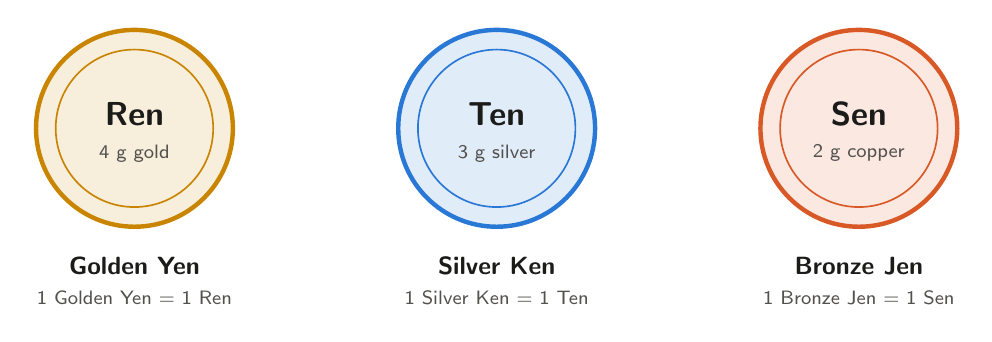
\begin{tikzpicture}[scale=1]
  \foreach \x/\c/\n/\m/\g in {0/yen/Golden Yen/Ren/4 g gold, 4.6/ken/Silver Ken/Ten/3 g silver, 9.2/jen/Bronze Jen/Sen/2 g copper}{
    \fill[\c!14] (\x,0) circle (1.25);
    \draw[\c,line width=1.6pt] (\x,0) circle (1.25);
    \draw[\c,line width=0.6pt] (\x,0) circle (1.0);
    \node[font=\sffamily\bfseries\large,color=ink] at (\x,0.18) {\m};
    \node[font=\sffamily\scriptsize,color=ink2] at (\x,-0.32) {\g};
    \node[font=\sffamily\small\bfseries,color=ink] at (\x,-1.75) {\n};
    \node[font=\sffamily\scriptsize,color=ink2] at (\x,-2.15) {1 \n{} = 1 \m};
  }
\end{tikzpicture}
\end{center}
\vspace{0.9cm}
{\sffamily\large\color{ink} Justus L. Ludovic\par}
\vfill
\begin{keybox}[Abstract]
\small
Zen is a monetary system of six coins: three physical coins of fixed metal weight, the gold Ren (4\,g), the silver Ten (3\,g) and the copper Sen (2\,g), and three public blockchains whose electronic coins are meant to be worth exactly one of them: Golden Yen, Silver Ken and Bronze Jen. No custodian holds the metal and no oracle reports its price. Each chain instead reads the value of its physical coin from its own payments: shops that price in coins pay exact sixths of a coin, and the chain compares those prices with ordinary payments to set the coin weight $S$, the number of base units that make one \JEN{} (or \KEN, or \YEN). Blocks are built by two kinds of work. Minters, who can be phones, hash a memory-hard puzzle to earn the right to prove groups of payments with zero-knowledge proofs and share the block's fees; miners seal the result with ordinary SHA-256 hardware and compete for new coins by a reward curve set by each metal's metallic ratio. This paper describes the whole system: the coins, the chains, Proof of Minting, mining and fork choice, block sizing by fee purity, the self-reading peg and its defences, the proof that turns a block, with its payments and its vault, channel, order and factory operations, into one 196-byte stamp, payment channels and channel factories, exchange between the chains, and Zen Net, a paid network layer on top. Every number in it comes from the draft protocol specification, measured prototypes or simulations, and each is marked as such. A Rust benchmark proves a block of 128 signed payments into one 196-byte proof that any node checks in 2--4\,ms, and a Rust test network now carries every operation of the system inside that same proof, with 583 rule-breaking tests that no operation circuit passes. Simulations show that the peg's defences turn an attack from a few thousand dollars of fees into millions of dollars of locked and lost capital with a hard ceiling of about 13\% a week, that a defender with half the attacker's money undoes an attack at about a twentieth of its cost, and that the peg converges to the physical coin's value only when most coin-priced shops set their prices from the metal. Taken together, physical and electronic coins on three linked chains form a self-correcting system: every node reads each chain's value nine ways from public data (payments, gram weights and the three exchanges), and an attack large enough to matter is detected and named within hours. Open problems are stated plainly.
\end{keybox}
\end{titlepage}

\tableofcontents
\vspace{0.6cm}
\begin{keybox}[How to read this paper]
\small
Zen is a design in progress. Each rule carries a status taken from the protocol specification (draft 0.2): \st{Decided}, \st{Proposed} (designed and simulated, not yet adopted), \st{Open} (a choice still to make) or \st{TBD} (not yet specified). Results are labelled \emph{measured} (prototype code on real hardware), \emph{devnet} (a multi-node test network of the Go prototype, versions Jen-0.5 to Jen-0.11) \emph{testnet} (the Rust node \texttt{zenproof}, a three-chain test network, rounds 1 to 55) or \emph{simulated} (a model, described in Appendix~\ref{app:sims}). Dollar figures assume Jen at one million payments a day, a typical payment of \$5, copper at \$13.80/kg and therefore a Sen worth \$0.0276. Nothing here is investment advice, and no part of the system has been audited.
\end{keybox}
\newpage

\section{Introduction}

Bitcoin showed that a peer-to-peer network can stop double spending without a trusted third party \cite{nakamoto}. Its unit, however, is too volatile to price goods or write contracts in \cite{yermack}. Every attempt since to give a cryptocurrency a stable unit trusts somebody: a custodian who holds the reference asset (e-gold, PAX Gold, Tether Gold), the publishers of a price feed (BitShares, Synthetix, Ampleforth), or a second token whose value is meant to absorb shocks (Terra, Basis, Iron Finance). Doing it in a fully decentralized way is still described as an open problem \cite{klagesmundt,caldarelli}. The custodians can fail or be closed, as e-gold was in 2008 \cite{egold-doj}; the feeds can be bribed or pushed, as Mango Markets' was \cite{mango}; and the second-token designs collapsed in runs \cite{terra}.

Zen takes a different route for one particular kind of stable unit: a unit of metal. It has six coins.

\begin{itemize}
\item Three \textbf{physical coins} of fixed weight: the gold \textbf{Ren} (4\,g), the silver \textbf{Ten} (3\,g) and the copper \textbf{Sen} (2\,g). They are ordinary metal, held privately, and worth what their metal is worth.
\item Three \textbf{electronic coins} on three independent public chains: \textbf{Golden Yen}, \textbf{Silver Ken} and \textbf{Bronze Jen}. The goal is $1~\YEN = 1~\REN$, $1~\KEN = 1~\TEN$ and $1~\JEN = 1~\SEN$.
\end{itemize}

Nobody holds metal for the electronic coins, and nobody reports a metal price to the chains. Each chain reads what its physical coin is worth from its own payments. Shops that price in coins (``this bread costs 6 Sen'') pay exact sixths of a coin; everybody else pays arbitrary amounts. Comparing the two tells the network how many of its base units one physical coin buys. The network then sets the weight of its electronic coin, $S$ base units, to that value. The off-chain fact, what a copper coin buys, still enters through people: Zen is an \emph{endogenous} oracle, not ``no oracle''. Fake payments cannot be ruled out without an authority \cite{douceur}, so the design does not try to forbid them. It prices them: each gram counts once, old money counts more than new, receivers post bonds, the reading moves at most 2.9\% a day, and once the three chains trade with each other an attacker must also beat the exchange.

The rest of Zen exists to make that measurement possible at scale and cheap enough for small payments:

\begin{itemize}
\item \textbf{Proof of Minting} (Section~\ref{sec:pom}): ordinary people, including phones, earn the right to prove groups of payments with zero-knowledge proofs by hashing a memory-hard puzzle. Their proofs build each block as a tree, so capacity grows with the number of minters, and they share the fees.
\item \textbf{Mining} (Section~\ref{sec:mining}): miners seal each minted block with SHA-256 over Bitcoin's exact 80-byte header, through ordinary Stratum pools, and win new coins on a curve set by each metal's metallic ratio. Fork choice counts both minting and sealing work.
\item \textbf{Purity} (Section~\ref{sec:purity}): each payment chooses its fee rate, its ``fineness'', and the average purity resizes the chain.
\item \textbf{The coin weight} (Section~\ref{sec:peg}): the self-reading peg and its layered defences.
\item \textbf{A self-correcting system} (Section~\ref{sec:selfcorrect}): why three linked currencies, each tied to a physical coin, can detect an attack, name the chain under attack and pull it back.
\item \textbf{Channels, factories and Zen Net} (Sections~\ref{sec:channels}--\ref{sec:zennet}): payments streamed off-chain across the three metals, and a paid network layer that uses them.
\end{itemize}

\paragraph{Contributions.} This paper (i) describes a complete design for metal-denominated electronic money with no custodian and no price feed; (ii) introduces Proof of Minting, a collaborative block-building scheme in which phones prove payments and share fees by work; (iii) specifies a peg read inside consensus from coin-priced payments, with a set of defences and their measured cost to an attacker; and (iv) reports prototype measurements, devnet tests and simulations for each of them, together with the problems that remain open (Section~\ref{sec:open}).

\paragraph{What Zen does not claim.} Zen measures value in metal. It does not stabilize the price of goods: metal standards gave long-run price stability alongside multi-decade deflations \cite{bordo,eichengreen}. It has no central bank or balance sheet, and every historical commodity scheme that actively stabilized prices had one \cite{bis2018,ussher}. Its claim is narrower: to give everybody a common, manipulation-resistant gram reference without a central party, so that metal becomes usable as a unit of account again.

%=====================================================================
\section{The system at a glance}\label{sec:overview}

\begin{figure}[tbp]
\centering
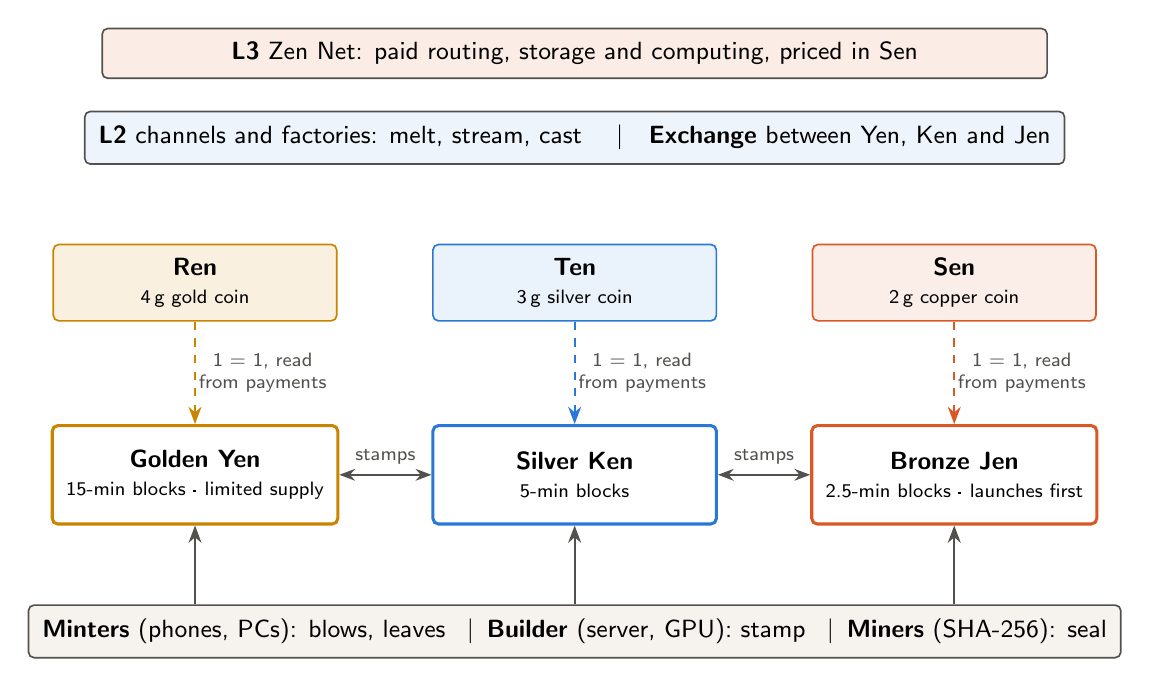
\begin{tikzpicture}[node distance=6mm and 6mm]
  % physical coins
  \node[box,fill=yen!12,draw=yen,minimum width=3.6cm] (ren) {\textbf{Ren}\\[-1pt]{\scriptsize 4\,g gold coin}};
  \node[box,fill=ken!10,draw=ken,minimum width=3.6cm,right=1.2cm of ren] (ten) {\textbf{Ten}\\[-1pt]{\scriptsize 3\,g silver coin}};
  \node[box,fill=jen!10,draw=jen,minimum width=3.6cm,right=1.2cm of ten] (sen) {\textbf{Sen}\\[-1pt]{\scriptsize 2\,g copper coin}};
  % chains
  \node[box,draw=yen,line width=1.1pt,minimum width=3.6cm,minimum height=1.25cm,below=1.3cm of ren] (yen) {\textbf{Golden Yen}\\[-1pt]{\scriptsize 15-min blocks \textperiodcentered{} limited supply}};
  \node[box,draw=ken,line width=1.1pt,minimum width=3.6cm,minimum height=1.25cm,below=1.3cm of ten] (ken) {\textbf{Silver Ken}\\[-1pt]{\scriptsize 5-min blocks}};
  \node[box,draw=jen,line width=1.1pt,minimum width=3.6cm,minimum height=1.25cm,below=1.3cm of sen] (jen) {\textbf{Bronze Jen}\\[-1pt]{\scriptsize 2.5-min blocks \textperiodcentered{} launches first}};
  \foreach \a/\b/\c in {ren/yen/yen,ten/ken/ken,sen/jen/jen}{
    \draw[arr,dashed,color=\c] (\a) -- node[lbl,right,fill=white,inner sep=1pt] {1 = 1, read\\from payments} (\b);
  }
  % work roles
  \node[box,fill=wash,below=1.0cm of ken,minimum width=12cm] (work) {\textbf{Minters} (phones, PCs): blows, leaves \enspace\textbar\enspace \textbf{Builder} (server, GPU): stamp \enspace\textbar\enspace \textbf{Miners} (SHA-256): seal};
  \foreach \c in {yen,ken,jen}{ \draw[arr] (work.north -| \c) -- (\c.south); }
  % upper layers
  \node[box,fill=bluewash,above=1.0cm of ten,minimum width=12cm] (l2) {\textbf{L2} channels and factories: melt, stream, cast \quad\textbar\quad \textbf{Exchange} between Yen, Ken and Jen};
  \node[box,fill=copperwash,above=4mm of l2,minimum width=12cm] (l3) {\textbf{L3} Zen Net: paid routing, storage and computing, priced in Sen};
  % cross check
  \draw[arr,{Stealth[length=2mm]}-{Stealth[length=2mm]},color=ink2] (yen.east) -- node[lbl,above] {stamps} (ken.west);
  \draw[arr,{Stealth[length=2mm]}-{Stealth[length=2mm]},color=ink2] (ken.east) -- node[lbl,above] {stamps} (jen.west);
\end{tikzpicture}
\caption{Zen's architecture. Three physical coins and three electronic chains; each chain reads its coin's value from its own payments. Minters and miners build every block; channels, the exchange and Zen Net sit on top. The chains verify each other's block proofs (stamps), but none depends on another for validity.}
\label{fig:arch}
\end{figure}

Figure~\ref{fig:arch} shows the parts and Table~\ref{tab:coins} the six coins. The physical coins are the reference and the store of value; the electronic coins are the medium of payment. The three chains are independent: each has its own work, its own block size and its own coin weight, and nothing in one chain's validity rules reads another chain's data \st{Decided}. They do follow each other's headers and check each other's block proofs (164 bytes, about 1\,ms each), so a payment on one chain can be verified on another without a bridge.

\begin{table}[htbp]
\centering\small
\begin{tabularx}{\textwidth}{l l l l Y}
\toprule
\textbf{Physical coin} & \textbf{Metal} & \textbf{Electronic coin} & \textbf{Chain role} & \textbf{Typical use}\\
\midrule
\textcolor{yen}{\textbf{Ren}} & 4\,g gold & Golden Yen (\YEN) & store of value & savings, large settlements, contracts\\
\textcolor{ken}{\textbf{Ten}} & 3\,g silver & Silver Ken (\KEN) & confirmation & salaries, mid-size payments, trade\\
\textcolor{jen}{\textbf{Sen}} & 2\,g copper & Bronze Jen (\JEN) & testing ground, launches first & everyday purchases, small change, streams\\
\bottomrule
\end{tabularx}
\caption{The six coins. The aim is $1~\YEN=1~\REN$, $1~\KEN=1~\TEN$ and $1~\JEN=1~\SEN$.}
\label{tab:coins}
\end{table}

\paragraph{Roles.} A \emph{user} sends and receives payments from a phone wallet. A \emph{minter} hashes the memory-hard blow puzzle and proves groups of payments; a phone can do this. A \emph{builder}, in practice a mining pool, turns the minters' leaves into a block and its stamp on a server with a GPU. A \emph{miner} seals blocks with SHA-256 hardware. A \emph{full node} keeps the state and serves it to minters. A \emph{stream node} runs channels on one or more metals and earns routing and exchange fees. Roles are switched on in one app \st{Decided in principle}.

\paragraph{Launch order.} Jen launches first. Ken starts when Jen's raw block reward first falls below one base unit (Jen block 729,328, about 3.5 years after Jen starts), and Yen when Ken's does (Ken block 21,138, about 73 days after Ken starts) \st{Decided}. Jen is therefore the proving ground for every rule; changes later pass to Ken and then to Yen with rising thresholds (Section~\ref{sec:upgrades}).

%=====================================================================
\section{Chain parameters and issuance}\label{sec:issuance}

Each metal is a separate chain with its own constants (Table~\ref{tab:params}). Three of them come from the \emph{metallic means}, the positive roots of $x^2 - m x - 1 = 0$ for the metallic order $m$:
\begin{equation}
r = \frac{m + \sqrt{m^2+4}}{2}, \qquad a = \frac{\ln 2}{\ln r}.
\end{equation}
Gold takes the golden ratio ($m=1$, $r=1.618$), silver the silver ratio ($m=2$, $r=2.414$) and bronze the bronze ratio ($m=3$, $r=3.303$). The ratio sets each chain's reward exponent $a$ and the spread of its random reward factor.

\begin{table}[htbp]
\centering\small
\begin{tabularx}{\textwidth}{Y r r r l}
\toprule
\textbf{Constant} & \textcolor{yen}{\textbf{Golden Yen}} & \textcolor{ken}{\textbf{Silver Ken}} & \textcolor{jen}{\textbf{Bronze Jen}} & \textbf{Status}\\
\midrule
Metallic order $m$ / ratio $r$ & 1 / 1.6180 & 2 / 2.4142 & 3 / 3.3028 & Decided\\
Reward exponent $a=\ln 2/\ln r$ & 1.440 & 0.786 & 0.580 & Decided\\
Block time & 15 min & 5 min & 2.5 min & Decided\\
Blocks per day & 96 & 288 & 576 & Decided\\
Data ceiling per block & 4 MB & 3 MB & 2 MB & Decided\\
Standard fee (purity target) & 0.1\% & 0.4\% & 1\% & Decided\\
Fee limits per payment & 0.01--2.5\% & 0.01--4.5\% & 0.01--6\% & Decided\\
Initial raw reward & 2,520 & 2,520 & 2,520 & Decided\\
Long-run supply & limited, $\approx$7,255 & grows $\approx N^{0.21}$ & grows $\approx N^{0.42}$ & Open (curve)\\
Smallest unit & $10^{-12}$ (pico) & $10^{-12}$ & $10^{-12}$ & Decided\\
Upgrade activation threshold & 90\% & 75\% & 60\% & Decided\\
Minter share of fees & 75\% & 75\% & 75\% & Open\\
\bottomrule
\end{tabularx}
\caption{Chain parameters (specification section 2).}
\label{tab:params}
\end{table}

\subsection{The reward curve}
The raw reward of block $N$ falls as a power of $N$:
\begin{equation}
\mathrm{Raw}(N) = 2520 \cdot N^{-a}.
\end{equation}
Because $a>1$ for gold, Yen's total supply converges, to about 7,255 coins; for silver and bronze $a<1$, so Ken and Jen grow forever, but ever more slowly, roughly as $N^{0.21}$ and $N^{0.42}$ (Figure~\ref{fig:supply}, Table~\ref{tab:supply}). Gold is scarce and final; copper keeps pace with an economy that keeps needing small change.

\begin{figure}[tbp]
\centering
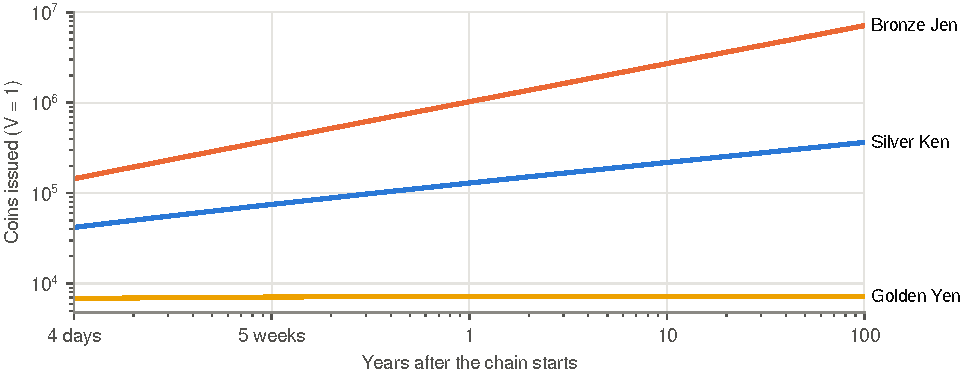
\includegraphics[width=\textwidth]{figs/supply.pdf}
\caption{Coins issued on each chain with the random factor $V=1$ in every block (computed from $\mathrm{Raw}(N)$; log scales). Yen approaches a limit of about 7,255 coins; Ken and Jen keep growing more slowly.}
\label{fig:supply}
\end{figure}

\begin{table}[htbp]
\centering\small
\begin{tabular}{l r r r}
\toprule
\textbf{Supply after} & \textbf{1 year} & \textbf{10 years} & \textbf{100 years}\\
\midrule
\textcolor{yen}{Golden Yen} & 7,198 & 7,234 & 7,247 (limit $\approx$7,255)\\
\textcolor{ken}{Silver Ken} & 129,000 & 218,000 & 362,000\\
\textcolor{jen}{Bronze Jen} & 1,026,000 & 2,706,000 & 7,121,000\\
\bottomrule
\end{tabular}
\caption{Supply with $V=1$ at every block (specification 5.5). The random factor raises the totals by its arithmetic mean, 1.12, 1.47 and 2.04 respectively.}
\label{tab:supply}
\end{table}

\subsection{A random factor that nobody can steer}
Each block's reward is multiplied by a random factor drawn from the \emph{next} block's seal, so no miner can know or influence its own draw \st{Decided}:
\begin{equation}
u = \frac{\mathrm{SHA256}(\mathrm{seal}_{N+1}\,\|\,\text{``reward''})}{2^{256}},\quad Z=\Phi^{-1}(u),\quad V = r^{Z},\quad \mathrm{Reward}(N) = \mathrm{Raw}(N)\cdot V .
\end{equation}
$V$ has a geometric mean (and median) of exactly 1, so a typical block follows the raw curve. All nodes compute it in integers: fixed constants for $\ln r$ and $a$, a fixed-point exponential, and a shared 65,536-entry table for $\Phi^{-1}$ and $r^Z$. There is no floating point in consensus.

\paragraph{The metallic split.} Once $V$ is known, the miner keeps the raw part of the new coins and the block's minters share the windfall above it, scaled by $1/r$ \st{Decided}:
\begin{equation}
\mathrm{Miner}(N) = \begin{cases}\mathrm{Raw}(N)\cdot V & V\le 1\\ \mathrm{Raw}(N)\cdot V^{1/r} & V>1\end{cases}\qquad \mathrm{Minters}(N) = \mathrm{Reward}(N)-\mathrm{Miner}(N).
\end{equation}
The miner's median income stays exactly $\mathrm{Raw}(N)$ and only windfalls are shared, so miners' income is steadier. Because the spread of $V$ grows with $r$, the minters' share grows from gold to bronze (Figure~\ref{fig:split}): on Jen, the everyday chain, minters receive more than half of the new coins on average.

\begin{figure}[htbp]
\centering
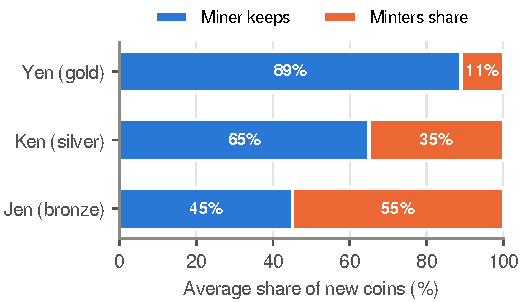
\includegraphics[width=0.62\textwidth]{figs/split.pdf}
\caption{Average split of new coins between the sealing miner and the block's minters (specification 5.4.1). In the top 1\% of Jen blocks $V$ reaches 16.1 and the miner keeps 2.3.}
\label{fig:split}
\end{figure}

%=====================================================================
\section{Accounts and payments}\label{sec:accounts}

Each chain keeps balances in a Merkle tree of accounts; each leaf is the hash of the account's address, balance and nonce, where the address is the hash of the public key, and its root is carried in every block header \st{Decided in principle}. The benchmark tree has depth 32, about 4.3 billion accounts. Every payment is public; privacy lives in the channel layer (Section~\ref{sec:channels}).

\paragraph{Payment format.} Inside a minted block a payment is about 13 bytes: a 4-byte sender index, a 4-byte receiver index, and the amount and fee as variable-length integers in base units (measured: 1,632 bytes for 128 payments). The nonce is implied by the sender's account and the signature is checked inside the proof, so neither is stored. In the pool, with its signature, a payment is about 100--140 bytes \st{TBD byte layout}.

\paragraph{Validity.} A payment is valid when its Schnorr signature on the EcGFp5 curve (prime order $n$, 319 bits; BabyJubjub EdDSA in the Go prototype) signs the Poseidon hash of the chain id, sender, receiver, amount, fee and nonce, with $s < n$; its nonce equals the sender's current nonce; the balance covers amount plus fee; its fee rate $\text{fee}/(\text{amount}+\text{fee})$ is inside the chain's limits; and the amount is at least the smallest payment (Section~\ref{sec:w}) \st{Decided}.

\paragraph{Purity: the payer chooses speed.} Each payment carries its \emph{fineness}, its fee rate expressed like the purity of metal: on Jen, from 940 (a 6\% fee) through the standard 990 (1\%) to 9999 (0.01\%). Minters take the highest fee first, counted in base units: 100~\JEN{} at 1\% (a fee of 1~\JEN) goes before 1~\JEN{} at 6\% (0.06~\JEN). The fineness only has to be inside the limits, so payers choose speed by the fee they pay \st{Decided, revised October 2026}. Under the earlier rule, which ranked by fee rate, on a busy Jen-0.6 devnet payments at 940 confirmed in a median of 15\,s, at 990 in 25\,s and at 9999 in 68\,s; the 9999 payments drained when traffic was quiet (Figure~\ref{fig:purity}). Sending 1~\JEN{} costs its purity in coins: 0.0638~\JEN{} at 940, 0.0101 at 990 and 0.0001 at 9999.

\begin{figure}[htbp]
\centering
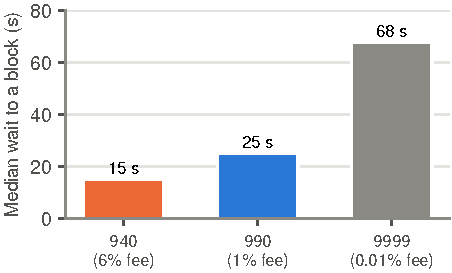
\includegraphics[width=0.55\textwidth]{figs/purity.pdf}
\caption{Fineness and speed on a busy Jen-0.6 devnet, when minters still ranked by fee rate: median time from sending to inclusion in a block (devnet).}
\label{fig:purity}
\end{figure}

\paragraph{New accounts.} A wallet is a key pair made offline; nothing is registered. An account appears in the tree the first time its address receives coins (a payment, a minting share or a mining reward). That first payment carries the 32-byte address once, about 45 bytes in the block; afterwards the account is a 4-byte index. The leaf then lives in the state, not in later blocks, until the account is closed. New accounts need no special spam rule: they compete for block space by fee like any payment, and the first amount must reach the smallest payment \st{Proposed}.

\paragraph{Closing an account.} A payment can close its sender's account with a signed flag: the balance must end at zero and the leaf is emptied, freeing the slot. A new account starts at nonce $\text{height}\times 2^{20}$, above any nonce an earlier account with the same key could have used, so its old signatures can never be replayed \st{Proposed, in the benchmark circuit}.

\paragraph{One address on all three chains.} The same key gives the same address on Yen, Ken and Jen, and a wallet shows it as one account with three balances. Each chain still keeps its own leaf for that address in its own tree, since no chain's rules read another chain's data, so a stall on one chain never freezes the others. Every signed message starts with the chain id, so a payment signed for one chain cannot be replayed on another even when the nonces match. In an exchange, ``to my Ken address'' is simply the trader's address, and a chain can check a payment on another chain against that chain's 196-byte stamp \st{Proposed, in the benchmark circuit}.

\paragraph{Two signatures, optional.} For shops and face-to-face payments, a payment request can ask for the receiver's signature too, and say who pays the fee and at what purity. Nobody can then push payments onto another account, and a wrong address cannot receive without agreeing. Ordinary sends, payroll and donations stay single-signature \st{Proposed}.

%=====================================================================
\section{Proof of Minting}\label{sec:pom}

Minters collaborate to turn waiting payments into one minted block, certified by small zero-knowledge proofs, and share the block's fees by the work they did. The vocabulary is metalworking: a minter's address is its \emph{hammer}, a hash attempt is a \emph{blow}, a proving task is a \emph{strike}, the final proof is the \emph{stamp} and a full minted block is an \emph{ingot}.

\begin{figure}[tbp]
\centering
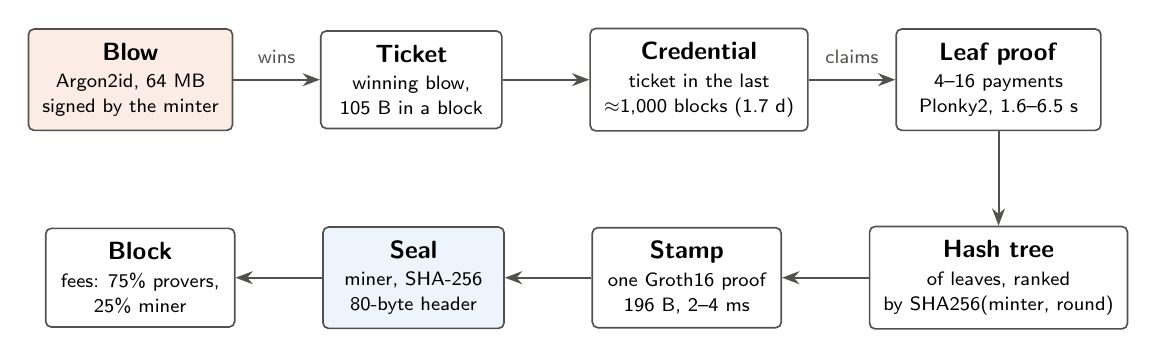
\begin{tikzpicture}[node distance=5mm and 11mm]
  \node[box,fill=copperwash,minimum width=2.4cm,minimum height=1.2cm] (blow) {\textbf{Blow}\\[-1pt]{\scriptsize Argon2id, 64 MB}\\[-2pt]{\scriptsize signed by the minter}};
  \node[box,right=of blow,minimum width=2.3cm,minimum height=1.2cm] (ticket) {\textbf{Ticket}\\[-1pt]{\scriptsize winning blow,}\\[-2pt]{\scriptsize 105 B in a block}};
  \node[box,right=of ticket,minimum width=2.4cm,minimum height=1.2cm] (cred) {\textbf{Credential}\\[-1pt]{\scriptsize ticket in the last}\\[-2pt]{\scriptsize $\approx$1,000 blocks (1.7 d)}};
  \node[box,right=of cred,minimum width=2.6cm,minimum height=1.2cm] (leaf) {\textbf{Leaf proof}\\[-1pt]{\scriptsize 4--16 payments}\\[-2pt]{\scriptsize Plonky2, 1.6--6.5 s}};
  \node[box,below=12mm of leaf,minimum width=2.6cm,minimum height=1.2cm] (tree) {\textbf{Hash tree}\\[-1pt]{\scriptsize of leaves, ranked}\\[-2pt]{\scriptsize by SHA256(minter, round)}};
  \node[box,left=of tree,minimum width=2.4cm,minimum height=1.2cm] (stamp) {\textbf{Stamp}\\[-1pt]{\scriptsize one Groth16 proof}\\[-2pt]{\scriptsize 196 B, 2--4 ms}};
  \node[box,left=of stamp,minimum width=2.3cm,minimum height=1.2cm,fill=bluewash] (seal) {\textbf{Seal}\\[-1pt]{\scriptsize miner, SHA-256}\\[-2pt]{\scriptsize 80-byte header}};
  \node[box,left=of seal,minimum width=2.4cm,minimum height=1.2cm] (block) {\textbf{Block}\\[-1pt]{\scriptsize fees: 75\% provers,}\\[-2pt]{\scriptsize 25\% miner}};
  \draw[arr] (blow) -- node[lbl,above=2pt] {wins} (ticket);
  \draw[arr] (ticket) -- (cred);
  \draw[arr] (cred) -- node[lbl,above=2pt] {claims} (leaf);
  \draw[arr] (leaf) -- (tree);
  \draw[arr] (tree) -- (stamp);
  \draw[arr] (stamp) -- (seal);
  \draw[arr] (seal) -- (block);
\end{tikzpicture}
\caption{Minting a block. Blows win tickets; a ticket in the recent chain is a credential; credentialed minters prove leaves of payments; leaves are merged into one stamp, and the miner seals the block.}
\label{fig:pipeline}
\end{figure}

\subsection{Blows}
A blow is one attempt at a memory-hard puzzle, signed with the minter's own account key, the key that also signs its payments \st{Decided; one key per person, Decided October 2026}:
\begin{align*}
m &= \mathrm{Poseidon}(\text{``ZenBlow''},\ \text{chain},\ \text{block}_{k-1},\ \text{nonce})\\
(e, s) &= \mathrm{Schnorr}_{\text{EcGFp5}}(\text{account key},\ m) \qquad \text{(deterministic)}\\
\mathit{blow} &= \mathrm{Argon2id}\big(\text{block}_{k-1}\,\|\,A\,\|\,\text{nonce}\,\|\,e\,\|\,s;\ \text{salt ``Zen-blow-v1''};\ 64\,\text{MB},\ 1\text{ pass},\ 1\text{ lane}\big)
\end{align*}
A blow wins when it is below the blow target. Everyone checks a winning blow with one signature check and one Argon2id run, with no state: the 105-byte ticket carries the compressed public key $A$ (41 bytes), the nonce, $e$ and $s$. The signature means only the key holder can make attempts for that key, and nobody can claim another minter's blow. Because the minting key is the account key, the ticket, the credential, the minters' coins and the leaf fees all reach one address, and handing the key to a pool would hand over the account's money: minting stays personal. Payment messages begin with the chain id and blow messages with the tag, so one signature never passes as the other, and a blow counts on one chain only. A minter may sign the same nonce twice, but each signature costs its own Argon2id run; a block counts one ticket per address and nonce. In Rust, on one server core, signing takes 1.2\,ms and an attempt 84\,ms; a node checks a ticket in about 75\,ms (measured). The 64\,MB of memory, refilled for every attempt, keeps dedicated chips from gaining a large advantage over phones and computers.

\begin{figure}[htbp]
\centering
\begin{minipage}[t]{0.48\textwidth}\centering
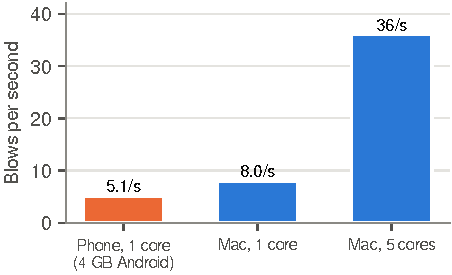
\includegraphics[width=\textwidth]{figs/blowbench.pdf}
\caption{Blows per second in a browser (Jen Minting Bench, 10 October 2026, measured). A phone takes 191--201\,ms per blow; a 10-core Mac 125\,ms per core. Neither slowed from heat over 4 minutes.}
\label{fig:blowbench}
\end{minipage}\hfill
\begin{minipage}[t]{0.48\textwidth}\centering
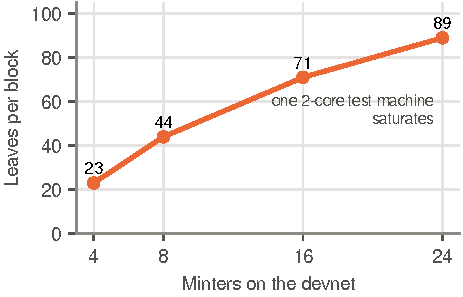
\includegraphics[width=\textwidth]{figs/capacity.pdf}
\caption{Collaborative minting on the Jen-0.8 devnet: leaves per block as minters are added (proving simulated at 2\,s per leaf). Capacity grows with minters until the single test machine saturates.}
\label{fig:capacity}
\end{minipage}
\end{figure}

The blow difficulty aims at a fixed number of winning blows per block, 24 on the real chains: after each block, $\text{new} = \text{old}\times(3\,\text{target} + \text{blows})/(4\,\text{target})$, limited to $\pm12.5\%$ per block \st{Decided}. More minters make blows harder, not blocks bigger. Checking 24 blows costs about 3\,s of one desktop core per 2.5-minute Jen block (measured).

\subsection{Tickets, credentials and the minting gate}
Every winning blow becomes a \emph{ticket}, a record of (public key, nonce, signature) of 105 bytes carried in the block \st{Decided, Jen-0.8; size from the Rust port}. Tickets do three things:
\begin{itemize}
\item \textbf{The minting gate.} A block is valid only with enough minting work: at least a third of the recent average minting work per block, counted as the sum of the blow difficulties, and never less than one blow at the current difficulty. A chain cannot meet the gate by lowering its own blow difficulty.
\item \textbf{New coins.} The minters' part of each block's new coins goes into a pool; each block's tickets share $1/32$ of the pool. On the devnet each minter's share of the minters' coins came within 2--4 points of its share of blows.
\item \textbf{Credentials.} A minter with a ticket in the chain within the last \textit{CredBlocks} blocks is credentialed: about 1,000 blocks, roughly 1.7 days, on the real chain. The ticket was verified when its block arrived, so checking a credential is a lookup.
\end{itemize}
In a three-minute quiet test with no payments sent, blocks kept coming every 16.7\,s with 51 tickets in 11 blocks (devnet): tickets keep the chain alive when nobody pays.

\subsection{Leaves: proving payments}
Any credentialed minter may claim waiting payments and prove \emph{leaves}, groups of 4 to 16 payments, one after another, as fast as its device allows \st{Decided, Jen-0.8}. Since October 2026 a leaf has two halves \st{Proposed, measured}:
\begin{itemize}
\item a \textbf{signature leaf}, proved by the minter, checks each payment's signature, the fee band and the floors in coins. It knows no balances and no tree, so any number of minters prove at the same time without knowing each other's leaves. Its public values are the hash of its signed payments with the minter's address, and $S$;
\item a \textbf{state leaf}, proved by the block builder, verifies one signature leaf inside it, repeats the signed fields (their hash must match, so the builder cannot change a payment, a nonce or the minter's address) and applies the payments to the account tree in order. A payment that no longer fits the state is \emph{skipped}: no change, no fee, absent from the block data.
\end{itemize}

\begin{table}[htbp]
\centering\small
\begin{tabular}{l r r r r}
\toprule
\textbf{Leaf size} & \textbf{Rows} & \textbf{Proving time} & \textbf{Memory} & \textbf{Proof}\\
\midrule
Signature leaf, 4 payments & $2^{12}$ & 1.4 s & 0.5 GB & 124 KB\\
Signature leaf, 16 payments & $2^{14}$ & 5--6 s & 0.9 GB & 143 KB\\
State leaf, 16 slots (builder) & $2^{13}$ & 2.7 s & 0.9 GB & 130 KB\\
\bottomrule
\end{tabular}
\caption{Leaf proofs, signatures checked inside the signature leaf: Plonky2 (FRI, no trusted setup, Poseidon over the Goldilocks field) on a 2-core server, October 2026 (measured; phones not yet tested). The Go prototype's Groth16 leaves (MiMC, gnark) took 3.8\,s for 4 payments and 13.9\,s for 16, with 164-byte proofs.}
\label{tab:leaf}
\end{table}

Leaves are ranked by $\mathrm{SHA256}(\text{minter identity}, \text{round}, \text{leaf})$. The rank fixes their order in the block and settles clashes. The block body is a hash tree of leaves and the miner seals its root. Each leaf's prover earns 75\% of that leaf's fees. With the stamp (Section~\ref{sec:stamp}) nodes check one proof per block instead of one per leaf; only blows cost an Argon2id check, so blows stay near 100 per block while leaves grow with the number of minters (Figure~\ref{fig:capacity}).

\paragraph{Fairness between fast and slow provers.} Two rules (Jen-0.10) keep one large prover, or a miner ordering its own leaves first, from filling a block: a \emph{leaf quota} (a minter may place at most $\tfrac54\times\text{cap}\times$ its share of tickets in the credential window, at least one leaf) and a \emph{split payment pool} (each payment falls in one bucket per round, $\mathrm{hash}(\text{payment},\text{round}) \bmod$ the number of credentialed minters, and each minter proves its own bucket first). On a six-node devnet with ten times more traffic than minters could prove, these rules cut wasted overlapping proofs from 78\% to 3\%, raised payments per block from 36 to 208, and cut the share of a prover 15 times faster than the rest from 99\% to 23\% of leaves (Figure~\ref{fig:ab}).

\begin{figure}[htbp]
\centering
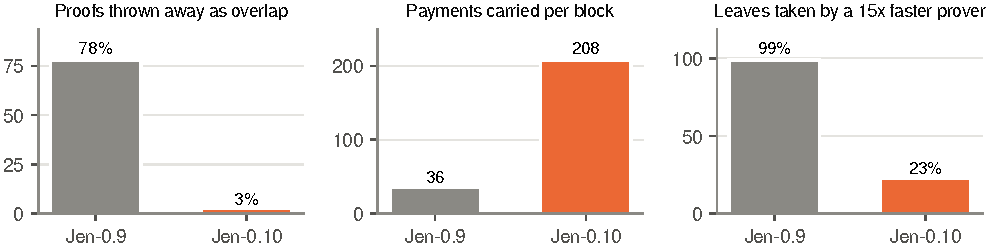
\includegraphics[width=\textwidth]{figs/ab.pdf}
\caption{Devnet A/B test, six nodes, traffic ten times what minters can prove: Jen-0.9 rules against Jen-0.10 (leaf quota and split pool). All nodes agreed and supply was exact in both (devnet).}
\label{fig:ab}
\end{figure}

\subsection{The same payment at two minters}
A payer can send two conflicting payments, with the same nonce, to two minters who prove them in parallel. Both proofs can be valid on their own; only one can be in the chain. Zen handles this in three layers:
\begin{enumerate}
\item The split pool sends all of a sender's payments in a round to the same bucket, so honest double proving is rare.
\item Within a block, leaves are applied in rank order. The builder's state leaf skips a payment whose (sender, nonce) is already used; only that payment is lost, and its minter earns no fee for it.
\item The clash is detected by (sender, nonce), not by payment ID, so two different payments with the same nonce always clash \st{Proposed for specification 4.10}.
\end{enumerate}
Signature leaves hold no state, so a conflicting payment costs its minter only that payment's fee, not the whole leaf. On a 128-slot block, a double spend (same sender, same nonce, two receivers) and a replayed payment were both skipped and the other payments applied (measured).

\subsection{Merging and the stamp}\label{sec:stamp}
In the Go prototype each node verifies every leaf proof (about 1\,ms each), which caps a block at 1,024 leaves, sized for a phone verifier \st{Decided, Jen-0.9}. A Rust benchmark written for this paper (October 2026) merges the leaves of a block into a single \emph{stamp} that any node checks in 2--4\,ms \st{Proposed, measured}. A block of 8 leaves of 16 payments goes through five stages (Figure~\ref{fig:zkpipeline}):
\begin{enumerate}
\item \textbf{Leaves} (Plonky2): signature leaves on minters' devices (16 payments, 5--6\,s), then state leaves on the builder (2.7\,s each), which apply the payments, move the state root and add the payouts (Section~\ref{sec:blockdata}).
\item \textbf{Merges} (Plonky2 recursion): a merge verifies two child proofs, checks that the left one's root after is the right one's root before, adds their fees and counts, and hashes their data commitments. Seven merges turn 8 leaves into one proof; each takes about 2.7\,s.
\item \textbf{Shrink} (Plonky2): the stamp is proved once more into a smaller circuit, $2^{13}$ rows.
\item \textbf{BN254 layer} (Plonky2): the same proof again, with its Merkle trees hashed by Poseidon over the BN254 field, so the next step can check it cheaply.
\item \textbf{Stamp} (Groth16 on BN254, gnark v0.16.4): a circuit of 4.2 million constraints verifies the whole BN254-layer proof and outputs 196 bytes. It needs 6\,GB and 96--112\,s on 2 cores; gnark's GPU prover (ICICLE) produces the same proof on an NVIDIA card.
\end{enumerate}

\begin{figure}[htbp]
\centering
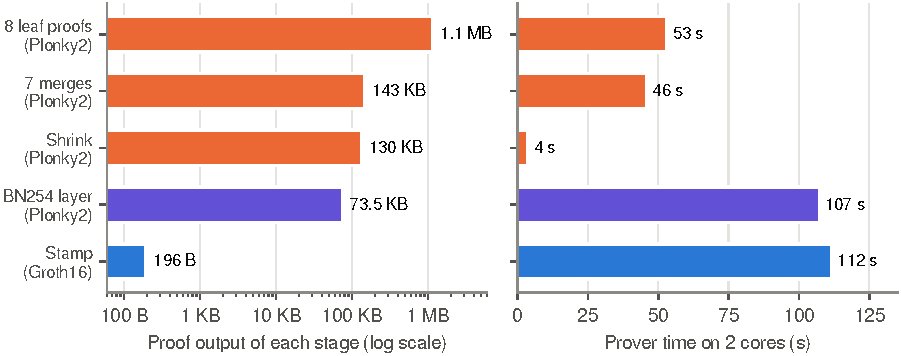
\includegraphics[width=\textwidth]{figs/zkpipeline.pdf}
\caption{A block of 128 signed payments from leaf proofs to one stamp: what each stage outputs (left, log scale) and the prover time it needs on a 2-core server (right). Orange: Plonky2 with Poseidon over Goldilocks; violet: Plonky2 with Poseidon over BN254; blue: Groth16. Leaves and merges run in parallel across minters; the times here are for one machine doing everything (measured, October 2026).}
\label{fig:zkpipeline}
\end{figure}

\paragraph{Why two proof systems.} Plonky2 proofs need no trusted setup and recurse cheaply, but each is 70--150\,KB. A Groth16 proof is 196 bytes and checks in milliseconds, but its key belongs to one circuit and needs a setup ceremony. Wrapping only the last step keeps the ceremony to one fixed circuit and keeps all the work that changes with traffic free of it. Without the wrap, the stamp is a 70\,KB Plonky2 proof with no setup at all, checked in about 3\,ms \st{Open: which one ships}. The Groth16 verifier is the open-source gnark verifier for Plonky2, ported to current Plonky2 and gnark; the port needed three changes, all from Plonky2 updates (the transcript now absorbs the FRI parameters, and two field generators changed).

\paragraph{Signatures inside the proof.} Proving is paid work and verification should stay cheap, so signatures are checked inside the leaf proofs and never published: a signature of 64 bytes or more per payment would be five times the 13-byte payment record. A custom gate computes $2P + Q$ on the curve in one operation, two per row, and one loop over the 319 bits of $s$ handles $s\cdot G$ and $e\cdot A$ together, which cut a 16-payment leaf from 30.7\,s and 4.3\,GB to about 5\,s and 0.6\,GB. The circuit checks that $s<n$, that the challenge is decoded canonically, that both points are on the curve, and that the addition formulas never meet an exceptional case. A forged signature produces no proof.

\paragraph{One key for every block size.} State-leaf proofs and merge proofs are built with exactly the same circuit shape: the same number of rows ($2^{13}$ since the leaf split), the same gate types and the same 84 public values. One \emph{universal merge} circuit can then verify either kind of child with a single verifier, switching only the key: the leaf's fixed key, or the merge circuit's own key, which every merge proof carries in its public values and must pass on to its parent. A lone child passes through. Any number of leaves therefore ends in a proof of the same circuit, and everything above it, including the Groth16 key, never changes. Blocks of 8, 3 and 1 leaves (128, 40 and 5 payments) produced identical final circuits and were proved and verified with one Groth16 key from one 20-minute setup; one block's proof checked against another block's public values was rejected. Merges got cheaper with the smaller shape, about 2.7\,s each. Within a leaf, unused slots are padding: they change no account, add no fee and are not counted.

\paragraph{Operations inside the stamp.} \st{Proposed, testnet} Payments are only part of a block. The chain also holds \emph{locks}, leaves of the account tree whose address is a digest of their terms: vaults, exchange orders and auctions, channels and channel factories (Sections~\ref{sec:channels} and~\ref{sec:exchange}). Each lock operation moves coins between an account and a lock, or between two states of one lock, so it changes the account tree like a payment does. Since the Rust test network reached this stage, four more leaf circuits sit beside the state leaf, one per family: \emph{vault} (make, claim, refund), \emph{channel} (make, fund, start, update, settle, close, streams, with up to eight point locks opened inside the circuit), \emph{order} (make, reserve, bid, reopen, return, claim) and \emph{factory} (up to eight members, make, fund, start, post, exit, exit now). Every leaf is built to the same shape as the state leaf ($2^{13}$ rows, the same gates, 84 public values), so the universal merge takes any mix of them: it now holds the verifier keys of the state leaf and the four operation leaves and picks one by a flag per child. A block with a payment, an order, a channel and a factory is one tree and one 196-byte stamp. Two format changes made this possible. Lock addresses and every signed message use Poseidon over field elements, not SHA-256, because one SHA-256 compression costs tens of thousands of gates; and the size of every list (point locks, factory members) has a fixed maximum. The block data hash commits to each operation in block order, as it does for payments.

The circuits check the rules a node checks (who may sign, the balances, the time windows, the update number, the shares, the opening of a point lock) with one deliberate exception: a few checks stay with the node, because they would cost many rows in the circuit. These are that a public key is in the right subgroup and matches its address, the sign of a curve point's $y$, that a new address is not already used, that the members of a factory are distinct, and the \emph{foreign payment proof} of an order claim. The last matters for the exchange: the circuit checks that the order is reserved, that the claim is inside the reservation, that the whole locked balance goes to the taker and that the sender signed the digest of the payment proof, but the other chain's header chain and block body are not in the circuit. Every node still checks that proof when it accepts the block. A stamp therefore tells a light client that the node rules were applied, and a full node re-checks the foreign payment; to make the stamp cover it would need the other chain's headers as public input and a block-body hash inside the circuit, a much larger step.

\paragraph{Testing the circuits against the node.} A circuit is sound if it cannot prove an operation that the node refuses. For each family a test walks a story of real operations and, at every step, tries to break it: one field changed (amount, fee, destination, sender, signature byte, terms, lock index, proof digest); the same operation tried six blocks before and after its true height, so that every time rule is tested on both sides of its edge; fee variants; and rule-breaking variants specific to the family (an unfunded make, an early reopen, a bid that does not beat the last, a claim after the window, an update number of zero, shares beyond the channel, a wrong point-lock scalar, an early exit, a forged member signature). A try passes if the circuit does not prove it, or proves exactly the honest operation. In all, 583 tries (vault 62, channel 181, order 196, factory 144) gave no failure. To check that the tests can see a bug, one rule (the order reopen window) was removed on purpose; eleven tries then failed, and the rule was restored (testnet). These tests are a probe and not a proof; they do not cover the node-only checks above, and they were run on a single-party setup (next paragraph).

\paragraph{The setup.} The Groth16 key of the operation-carrying circuit was made on one machine for the test network: 4.2 million constraints, a 2\,GB proving key, a 1,008-byte verifying key, about 17 minutes. Whoever runs such a setup could keep its secret randomness and forge stamps, so this key is for testing only. A launch needs a public multi-party ceremony for exactly this circuit \st{Open}; the 70\,KB Plonky2 stamp, which needs none, remains the fallback.

\paragraph{Who proves what, and when.} Every block carries its stamp \st{Decided, October 2026}. The protocol names no machine: a builder too slow to finish the stamp misses the block, and someone faster seals it. Minters prove signature leaves on phones and PCs; the builder, in practice a mining pool, proves state leaves, merges and the BN254 layer on server cores and the Groth16 stamp on an NVIDIA GPU through gnark's ICICLE backend, which reads the same proving key and produces the same 196-byte proof; miners seal with SHA-256 ASICs. On 2 cores the builder's work takes about 3.7 minutes; the target is about 60 seconds after the last leaf, inside Jen's 2.5-minute block. The GPU prover is built but not yet measured, so this target is open until a benchmark on a many-core GPU server. The peg's account fields (Section~\ref{sec:defences}) are in the account leaf and the state leaf (Rust, round 13), and none of the circuits is audited.

\subsection{Block data and node checks}\label{sec:blockdata}
A stamp proves that the new state root is right, but a root alone tells nobody their balance, and the next prover needs the whole tree. So every block publishes its payments (without signatures), and the stamp \emph{commits} to them: each leaf hashes its slot entries (unused flag, sender, receiver, amount, fee, new-account and close flags, a new account's address) and its prover's address, and each merge hashes the two child hashes. The stamp's 16 public values are the root before and after, the fee total, the payment count, this data hash, $S$ and the block height \st{Proposed, measured}. A node accepts a block when, in order:
\begin{enumerate}
\item its root before equals the previous block's root after;
\item the stamp verifies with the 16 public values;
\item the payment bytes decode cleanly (minimal integers, no trailing bytes);
\item replaying the payments on its own copy of the state, with the rules of Section~\ref{sec:accounts}, gives the same root after, fee total, count and data hash.
\end{enumerate}
A block of 128 payments measured 1,940 bytes: 1,632 of payments (12.6 bytes each), 13 of header and counts, 112 of public values and 196 of stamp, about 15 bytes per payment. With the version-2 leaf header (37 bytes per leaf: count, new-account and close masks, prover address) and 21 payments creating accounts, a block of 128 payments carried 2,596 bytes of data. Changing one byte of the payment data made the replay disagree. The signed message includes the sender's nonce and the proof increments it, so a payment re-submitted with its original signature is skipped and never applied twice.

\paragraph{Minters are paid by lottery.} The minters' share of a block goes straight to that block's 24 winning tickets, equal shares each, one credit per address; no node keeps a ledger of what minters are owed. The number of credits a block spends on minters is therefore at most 24, whether there are a hundred minters or a billion: more minters only raise the difficulty. In a simulation of 100 to 300,000 minters, a block carried 18 to 24 credits, and pay followed work (the top 1\% of minters earned 35.6\% of the pay for 35.2\% of the work). The price is variance: a small solo minter wins rarely, about once in (minters $/$ 24) blocks, so steady income comes from minting pools, which are ordinary addresses that split what they win with ordinary payments. An earlier design that paid every minter once every 32 blocks was dropped, because its saving fell to 1.6$\times$ at 10,000 minters \st{Decided}.

\paragraph{Payouts inside the proof.} A slot that a signature leaf left empty can carry a \emph{credit}: no sender, no signature, an amount added to an account, which is created on first receipt \st{Proposed, measured}. Every node computes the payouts a block owes: half of each leaf's fees goes into a fee pool, 75\% of the rest to the leaf's prover and the remainder to the miner; the pool pays 1/32 of what it held per block, 75\% to the block's provers and the rest to the miner; rewards owed from block $h-2$ come first (75/25 \st{Open}). A block is valid only if its credits, in order, are exactly that list, and the proof shows that each one reached the account tree. A leaf with no payments is credit-only and reuses one empty signature leaf. In a 128-slot block, 110 payments and 11 credits, one of them opening a minter's account, took 2,401 bytes (version 4: each leaf header carries payment, credit, new-account and close masks and the prover, 40 bytes). A builder that paid one unit too much produced a valid proof, and nodes rejected the block (measured).

\begin{figure}[tbp]
\centering
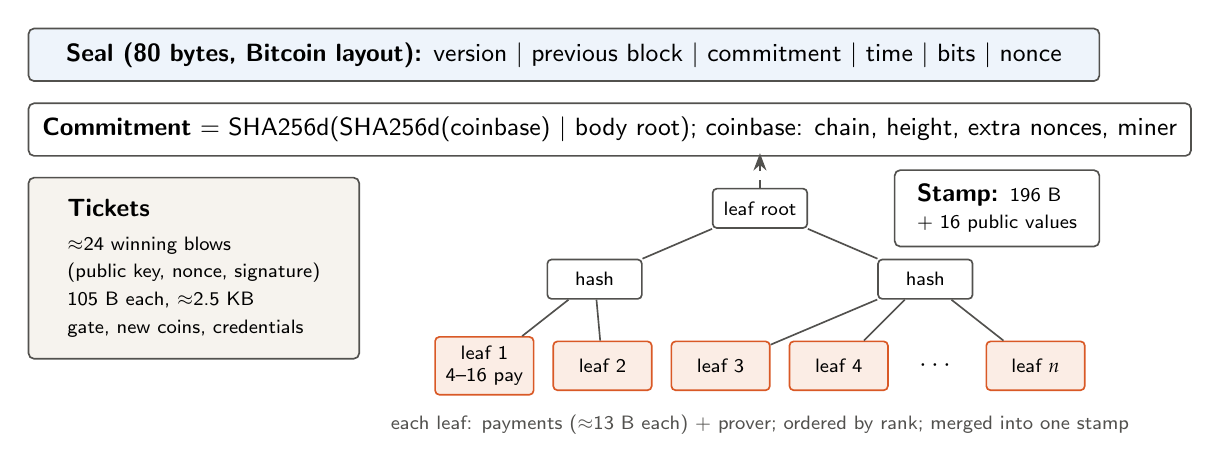
\begin{tikzpicture}[
  lf/.style={draw=jen,fill=copperwash,rounded corners=1.5pt,minimum width=1.25cm,minimum height=0.62cm,font=\sffamily\scriptsize,align=center,line width=0.6pt},
  hn/.style={draw=ink2,fill=white,rounded corners=1.5pt,minimum width=1.2cm,minimum height=0.5cm,font=\sffamily\scriptsize,line width=0.6pt}]
  % header
  \node[box,fill=bluewash,minimum width=13.6cm,align=left,anchor=west] (hdr) at (0,4.3) {\textbf{Seal (80 bytes, Bitcoin layout):} version \textbar{} previous block \textbar{} commitment \textbar{} time \textbar{} bits \textbar{} nonce};
  \node[box,minimum width=13.6cm,align=left,anchor=west] (com) at (0,3.35) {\textbf{Commitment} = SHA256d(SHA256d(coinbase) \textbar{} body root); coinbase: chain, height, extra nonces, miner};
  % tickets
  \node[box,fill=wash,minimum width=4.2cm,minimum height=2.3cm,anchor=north west,align=left] (tk) at (0,2.75) {\textbf{Tickets}\\[1pt]{\scriptsize $\approx$24 winning blows}\\[-1pt]{\scriptsize (public key, nonce, signature)}\\[-1pt]{\scriptsize 105 B each, $\approx$2.5 KB}\\[-1pt]{\scriptsize gate, new coins, credentials}};
  % tree
  \node[hn] (r) at (9.3,2.35) {leaf root};
  \node[hn] (a) at (7.2,1.45) {hash};
  \node[hn] (b) at (11.4,1.45) {hash};
  \node[lf] (l1) at (5.8,0.35) {leaf 1\\4--16 pay};
  \node[lf] (l2) at (7.3,0.35) {leaf 2};
  \node[lf] (l3) at (8.8,0.35) {leaf 3};
  \node[lf] (l4) at (10.3,0.35) {leaf 4};
  \node[font=\sffamily\small] at (11.55,0.35) {$\cdots$};
  \node[lf] (l5) at (12.8,0.35) {leaf $n$};
  \draw[line width=0.6pt,color=ink2] (r) -- (a); \draw[line width=0.6pt,color=ink2] (r) -- (b);
  \draw[line width=0.6pt,color=ink2] (a) -- (l1); \draw[line width=0.6pt,color=ink2] (a) -- (l2);
  \draw[line width=0.6pt,color=ink2] (b) -- (l3); \draw[line width=0.6pt,color=ink2] (b) -- (l4); \draw[line width=0.6pt,color=ink2] (b) -- (l5);
  \node[lbl,anchor=north] at (9.3,-0.15) {each leaf: payments ($\approx$13 B each) + prover; ordered by rank; merged into one stamp};
  \draw[arr,dashed] (r.north) -- (9.3,3.05);
  \node[box,minimum width=2.6cm,anchor=west,align=left] at (11.0,2.35) {\textbf{Stamp:} \scriptsize 196 B\\[-1pt]\scriptsize + 16 public values};
\end{tikzpicture}
\caption{Structure of a minted block. The miner's 80-byte seal commits to everything else, so miners cannot change a minted block. For example, 24 tickets (2.5\,KB), 660 payments (about 8.6\,KB at 13\,B each) and one stamp with its public values (324\,B) make a block of about 11.5\,KB (estimate).}
\label{fig:block}
\end{figure}

%=====================================================================
\section{Mining and consensus}\label{sec:mining}

\subsection{The seal}
Miners seal each minted block with double SHA-256 over Bitcoin's exact 80-byte header: version, previous block, a commitment, time, compact difficulty bits and a 32-bit nonce, in Bitcoin's byte order \st{Decided, Jen-0.5; Bitcoin-exact since October 2026}. The commitment is built as a Bitcoin merkle root over a one-transaction coinbase and one branch, $\mathrm{SHA256d}(\mathrm{SHA256d}(\text{coinbase})\,\|\,\text{body root})$: the coinbase holds the chain, the height, the pool's and miner's extra nonces and the miner's address, and the body root hashes everything minted (Figure~\ref{fig:block}), so a miner cannot alter a minted block. This is exactly what Stratum v1 pools and their miners compute, so existing SHA-256 chips, firmware and pools seal Zen blocks unchanged, version rolling included; a pool puts its own address in the coinbase and pays its miners as it does for Bitcoin. No private key is needed and pools are allowed. Our header code reproduces Bitcoin's genesis block hash; a miner that knew only Stratum found a seal the node accepted, and a seal reused for a changed block, a swapped miner address and a seal shown to another chain were rejected (measured). Mining and minting are deliberately different: minting is personal, memory-hard and phone-friendly; sealing is anonymous, poolable and uses the world's largest installed hashing base.

\subsection{Two-factor fork choice}
The chain with the most total weight wins; at equal height the lower seal hash wins \st{Decided, Jen-0.5}. Each block's weight counts both kinds of work:
\begin{equation}
\mathrm{Weight}(B) = D_{\mathrm{seal}}\cdot\frac{\min(\mathrm{blows}_B,\ 2\bar b)}{\bar b},\qquad \bar b \leftarrow \bar b + \frac{\mathrm{blows}_B - \bar b}{32}.
\end{equation}
A chain sealed with much hashing but little minting weighs little. In hidden-chain attacks on the Jen-0.5 devnet, an attacker with three times the honest sealing power built in secret for four minutes and then published. With seal work alone, an attacker with half the honest minting made honest nodes abandon 17 blocks; with two-factor weight the same attacker reached only 59\% of the honest weight and failed, though its chain was three blocks longer (Figure~\ref{fig:hidden}).

\begin{figure}[htbp]
\centering
\begin{minipage}[t]{0.48\textwidth}\centering
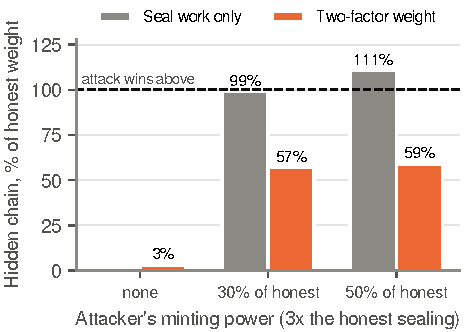
\includegraphics[width=\textwidth]{figs/hidden.pdf}
\caption{Hidden-chain attacks on the Jen-0.5 devnet with three times the honest sealing power. Bars show the hidden chain's weight as a share of the honest chain's (devnet).}
\label{fig:hidden}
\end{minipage}\hfill
\begin{minipage}[t]{0.48\textwidth}\centering
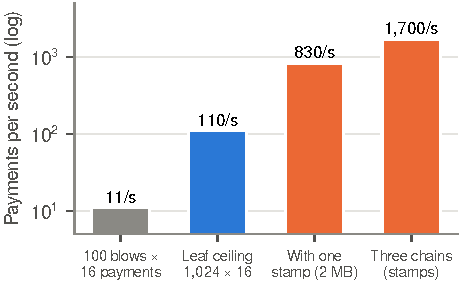
\includegraphics[width=\textwidth]{figs/throughput.pdf}
\caption{Jen throughput levers (estimates). Today, 24 blows each carrying up to 16 payments; then the 1,024-leaf ceiling; then one stamp per block, filling the 2\,MB ceiling; then all three chains.}
\label{fig:throughput}
\end{minipage}
\end{figure}

\subsection{Difficulty and launch}
Two difficulties run side by side: the blow difficulty keeps winning blows near their target per block (Section~\ref{sec:pom}), and the seal difficulty keeps each chain at its block time \st{TBD numbers}. A retarget that only acts when a block arrives has a weakness at launch and when miners leave suddenly: if the difficulty is set for far more hashing than is present, the next block is slow, and each slow block only lowers the difficulty one step. Zen therefore proposes a \emph{time-based} difficulty (in the style of ASERT): the target a block must meet is computed from how far the chain is ahead of or behind its schedule, so the difficulty keeps falling while nobody finds a block \st{Proposed}:
\begin{equation}
D(t) = D_{\mathrm{ref}}\cdot 2^{\,(N T - t)/h},
\end{equation}
where $N$ is the number of blocks since the reference block, $T$ the block time, $t$ the time since the reference block and $h$ the half-life. Figure~\ref{fig:launch} compares the two rules on Jen in a simple simulation made for this paper. With a genesis difficulty set for fifty times the hashing that shows up, per-block retargeting needs about 28 hours to reach block 100 instead of about 4; the time-based rule with a one-hour half-life needs about 10. When 90\% of the hashing leaves suddenly, per-block retargeting takes about 10.6 hours to reach block 100 against 4.4 for the time-based rule. The same rule applies to the blow target, so a minting gate never blocks a young chain with few minters.

\begin{figure}[htbp]
\centering
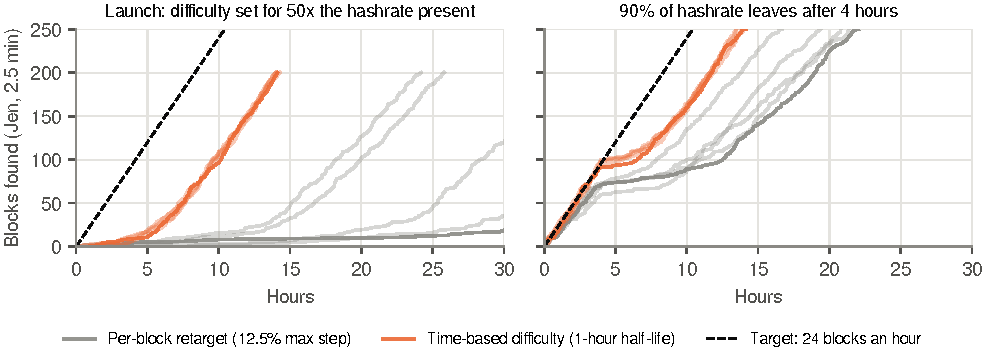
\includegraphics[width=\textwidth]{figs/launch.pdf}
\caption{Launch and hashrate-drop simulation for Jen (five runs per rule, Poisson block discovery; simulated for this paper, Appendix~\ref{app:sims}). Grey: retarget only when a block arrives, at most 12.5\% per block. Orange: time-based difficulty with a one-hour half-life.}
\label{fig:launch}
\end{figure}

\paragraph{Throughput.} A Jen block carries 24 winning blows. With up to 16 payments per blow that is 384 payments per 150-second block, about 2.6 payments per second. Leaves are not tied to blows once minters are credentialed, so the real ceiling is the 1,024-leaf verification limit: up to 16,384 payments a block, about 110 per second. With one stamp per block (benchmarked in Section~\ref{sec:stamp}) the limit becomes the 2\,MB data ceiling at about 16 bytes a payment: about 125,000 payments a block, 830 per second on Jen and about 1,700 per second across the three chains (Figure~\ref{fig:throughput}). Payments beyond that move to channels.

%=====================================================================
\section{Block size and purity}\label{sec:purity}

Each chain resizes itself from the fee rates its payers choose. \emph{Purity} is the fees paid divided by the value transacted over a day of payments (96, 288 or 576 blocks), so each payment counts by its size and the target is the standard fee, 1\% on Jen \st{Decided, revised October 2026}. An earlier rule took the geometric mean of fee rates counted per payment; a flood of tiny payments at the top rate could move it for almost nothing, and minters now also rank payments by fee, not by fee rate (Section~\ref{sec:accounts}). It answers one question: are payers paying for speed?

\begin{itemize}
\item \textbf{Grow} when the recent fee rate is above 1.02\% on Jen and blocks average over 90\% full, each block's fullness counted against what the cap allows for the time the block took (at least a quarter of the target time) \st{Decided, Jen-0.11}.
\item \textbf{Hold} when fees are high but blocks are not full: the problem is too few provers, not too little room.
\item \textbf{Shrink} only when fees are at the standard rate and blocks are under 60\% full.
\end{itemize}

Steps on Jen are $+0.3\%$ per block to grow and $-0.12\%$ to shrink. Hard ceilings are 4\,MB (Yen), 3\,MB (Ken) and 2\,MB (Jen); until nodes check one proof per block, the 1,024-leaf verification limit is lower. Faking congestion costs money: half of each fee goes into a pool that pays $1/32$ of itself to each later block, so fees paid to oneself are partly lost. On the Jen-0.7 devnet, capacity per blow rose from 4 to 16 payments when 70\% of payments chose fineness 940 and fell back to 4 when 60\% chose 9999.

\paragraph{No cross-chain consensus dependency.} A joint resize of the three chains was considered and dropped: Jen, the cheapest chain to fill with fake fees, could then resize Yen, and a stall on Jen would spread. Demand that Yen cannot hold instead flows down to Ken and Jen through higher Yen fees, and wallets route payments through the cheaper metals \st{Decided}.

%=====================================================================
\FloatBarrier
\section{The coin weight: one \JEN{} is one \SEN}\label{sec:peg}

This section is the heart of Zen. Balances, fees and rewards are counted in fixed base units (pico). A coin weighs $S$ base units, and $S$ is what the network reads the physical coin to be worth, so $1~\JEN = 1~\SEN$ by definition of $S$; each chain has its own $S$. The section explains how $S$ is read, how the reading is defended, what an attack costs, and how fast $S$ reaches the truth.

\subsection{Fee limits in coins}\label{sec:w}
The fee limits are set in coins, so they follow $S$ \st{Decided, revised October 2026}. The smallest fee is 0.01 coin, and the smallest payment is the smallest fee divided by the chain's top fee rate, so the smallest payment at the top rate pays exactly the smallest fee:

\begin{center}\small
\begin{tabular}{l r r r}
\toprule
 & \textbf{Golden Yen} & \textbf{Silver Ken} & \textbf{Bronze Jen}\\
\midrule
Fee limits & 0.01\%--2.5\% & 0.01\%--4.5\% & 0.01\%--6\%\\
Smallest fee & 0.01~\YEN & 0.01~\KEN & 0.01~\JEN\\
Smallest payment & 0.4~\YEN & $\tfrac29$~\KEN & $\tfrac16$~\JEN\\
\bottomrule
\end{tabular}
\end{center}

With a Sen at \$0.0276, the smallest Jen payment is about \$0.005 and the smallest fee about \$0.0003. The resize (Section~\ref{sec:purity}) keeps the price of block space near the standard fee, so a payment costs about its standard rate of what it moves, however the chain is used.

An earlier draft set these limits from $W$, the typical payment size. A floor tied to payment sizes rises when large payments dominate: a typical payment of 600,000~\JEN{} would make the smallest payment 1,000~\JEN, about \$27, and lock small payers out just as the chain became popular. $W$ also had its own attack (a fifth of all payments for a week moved it by up to 50\% in simulation). Setting the limits in coins removes both. The cost is that the limits follow $S$, so an attack on the peg moves them too, but only within $S$'s band: at worst from $\tfrac16$ to about $\tfrac19$ or $\tfrac14$ Sen. Before the peg converges, the floor floats with whatever a Jen is worth, and the launch rules may start lower.

\subsection{Reading $S$ from coin-priced payments}
Payments come in two modes, told apart by the amount alone \st{Decided in principle}:
\begin{itemize}
\item \textbf{Coin-priced} (``Sen-priced''): a shop prices in coins. The amount is an exact whole number of sixths of the $S$ of one of the last 8 blocks, so the network reads the price in Sen. A converted amount essentially never lands on an exact sixth by chance: none of 200,000 random amounts did in the Jen-0.9 test.
\item \textbf{Ordinary}: any other amount, for example converted from another currency. The network reads its value in base units.
\end{itemize}

The two modes describe the same goods. If the typical coin-priced basket costs $p$ Sen and the typical ordinary payment is worth $v$ base units, a Sen is worth about $v/p$ base units, and that is where $S$ moves:
\begin{equation}
S_{\text{target}} = \frac{\text{typical ordinary value (base units)}}{\text{typical coin-priced price (in coins)}} .
\end{equation}
The physical metal enters at exactly one point: shops that set their coin prices from what the physical coin buys. A shop that converts from the network's own rate merely reports $S$ back to itself (Section~\ref{sec:converge}).

\begin{figure}[tbp]
\centering
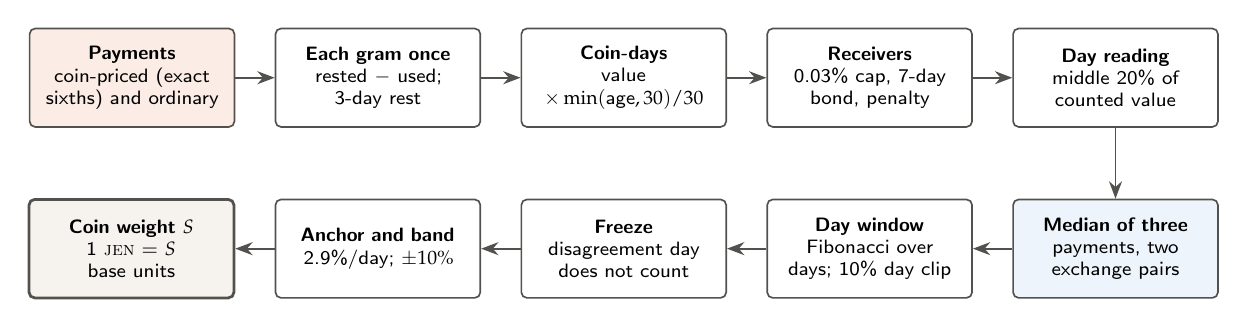
\begin{tikzpicture}[node distance=4mm and 5mm,
  st/.style={box,minimum height=1.25cm,text width=2.25cm,font=\sffamily\scriptsize}]
  \node[st,fill=copperwash] (pay) {\textbf{Payments}\\ coin-priced (exact sixths) and ordinary};
  \node[st,right=of pay] (once) {\textbf{Each gram once}\\ rested $-$ used; 3-day rest};
  \node[st,right=of once] (cd) {\textbf{Coin-days}\\ value $\times\min(\text{age},30)/30$};
  \node[st,right=of cd] (rcv) {\textbf{Receivers}\\ 0.03\% cap, 7-day bond, penalty};
  \node[st,right=of rcv] (mid) {\textbf{Day reading}\\ middle 20\% of counted value};
  \node[st,below=9mm of mid,fill=bluewash] (med) {\textbf{Median of three}\\ payments, two exchange pairs};
  \node[st,left=of med] (win) {\textbf{Day window}\\ Fibonacci over days; 10\% day clip};
  \node[st,left=of win] (frz) {\textbf{Freeze}\\ disagreement day does not count};
  \node[st,left=of frz] (anc) {\textbf{Anchor and band}\\ 2.9\%/day; $\pm10\%$};
  \node[st,left=of anc,fill=wash,line width=1pt] (S) {\textbf{Coin weight $S$}\\ 1 \JEN{} = $S$ base units};
  \draw[arr] (pay) -- (once); \draw[arr] (once) -- (cd); \draw[arr] (cd) -- (rcv); \draw[arr] (rcv) -- (mid);
  \draw[arr] (mid) -- (med); \draw[arr] (med) -- (win); \draw[arr] (win) -- (frz); \draw[arr] (frz) -- (anc); \draw[arr] (anc) -- (S);
\end{tikzpicture}
\caption{How a chain reads its coin weight. Each stage removes one way to fake the reading. The exchange stage applies once Ken and Yen exist; until then Jen relies on its own payments.}
\label{fig:reading}
\end{figure}

\subsection{The defences}\label{sec:defences}
A naive reading is cheap to move. In the Jen-0.11 devnet, one node sending fake coin-priced payments to its own users dragged 1~\JEN{} from 1.0 to 0.31~Sen in 40 blocks. The defences below, simulated in the market model of Appendix~\ref{app:sims}, each remove one way to fake the reading (Figure~\ref{fig:reading}) \st{Proposed, simulated}.

\paragraph{Each gram counts once.} Every account carries three numbers: \emph{rested} (money unmoved for the rest period, 3 days proposed), \emph{fresh} (money received since, with its arrival day) and \emph{used} (rested money already counted this period). A payment counts toward $S$ only up to rested minus used. The payment itself always goes through. The numbers change only when the account sends or receives, and the leaf proof checks them together with the balance, so nothing private is revealed. Money paid around in a loop counts once per rest period. The rules are exact: before a send or receive the account is settled at the block's day (fresh money older than the rest period becomes rested; the used number restarts in a new 3-day period); a payment spends fresh money first, counts the smaller of its amount and rested minus used, and rested money that leaves is the used money first; a receipt adds fresh money and restarts the clock of all fresh money in the account, which is conservative. The account leaf holds five more numbers (11 field elements) and the state leaf proves every transition; a builder that claimed more rested money than the leaf holds produced no proof, and a node replaying the block counts the same amounts as the builder (measured; block data is unchanged, 2,401 bytes for the test block, and the state leaf stays at $2^{13}$ rows, 2.6\,s) \st{Proposed, measured}.

\paragraph{Value weighting.} Because money counts once, the reading weighs payments by value: each day it takes the middle 20\% of counted value, by log price on the coin-priced side and by log value on the ordinary side. Each block adds its counted payments to two fixed histograms of about 1,000 bins; at the end of the day one number per side is kept. Tiny fake payments weigh almost nothing.

\paragraph{Coin-days.} A counted payment weighs its value times $\min(\text{age},30)/30$, where age is how many days its money rested, as in Peercoin's coin age \cite{peercoin}. Honest customers mostly spend money held for weeks and count close to fully. An attacker who cycles money counts at most $C/30$ a day for $C$ dollars, whatever his cycle.

\paragraph{Day window, clip, anchor and band.} The day readings enter a window with Fibonacci weights over days (Figure~\ref{fig:window}). A day's reading may differ from the window before it by at most 10\%. A slow \emph{anchor} follows $S$ by at most 0.005\% a block (2.9\% a day), and $S$ must stay within $\pm10\%$ of the anchor. This is the one hard limit: whatever an attacker spends, $S$ moves at most about 13\% in a week and 37\% in a month.

\begin{figure}[htbp]
\centering
\begin{minipage}[t]{0.42\textwidth}\centering
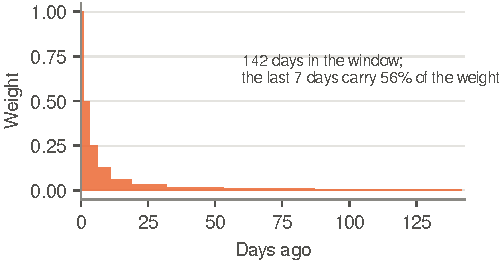
\includegraphics[width=\textwidth]{figs/window.pdf}
\caption{Fibonacci day weights: 1 for the last day, $\tfrac12$ for the two before, $\tfrac14$ for the next three, and so on.}
\label{fig:window}
\end{minipage}\hfill
\begin{minipage}[t]{0.54\textwidth}\centering
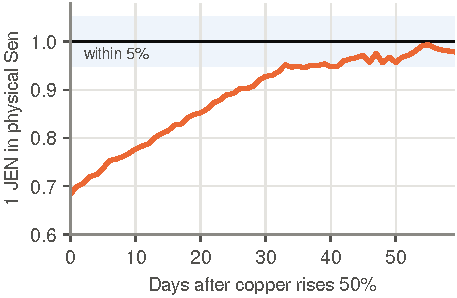
\includegraphics[width=\textwidth]{figs/copper.pdf}
\caption{A genuine change: copper rises 50\% and the network follows. With window, clip, anchor and band, 1~\JEN{} is back within 5\% of 1~\SEN{} in about 39 days (simulated).}
\label{fig:copper}
\end{minipage}
\end{figure}

\paragraph{Receiver cap and bond.} A receiving account counts for at most 0.03\% of the day's counted coin-priced value. It counts at all only if it has held a bond for 7 days (base about \$1,000, set as a share of traffic). Each bonded receiver has one vote, its own price change against its own past. When the value-weighted change differs from the median vote by more than 3\%, the bond required grows 20\% a day, up to 20 times; otherwise it shrinks 5\% a day back to the base. A genuine price move shifts all shops alike and does not raise the bond.

\paragraph{Bond penalty.} Each bonded receiver's 30-day price change is compared with the median receiver's. A receiver more than 15\% away loses 2\% of its bond a day, burned. In simulation 0.1\% of honest shops were ever hit. An attacker must pay the penalty or keep his payments within 15\% of the typical price, which needs far more money for the same push.

\paragraph{Freeze on disagreement.} When receivers disagree beyond the trigger, the day does not count and $S$ holds \st{Proposed}. An alternative, reading the day from the median receiver vote, was rejected: an attacker with many bonded accounts (about 2,600 for \$25M) outvotes the 730 honest ones and reached a 39\% move.

\paragraph{Standard fee and settlement.} Only payments paying at least the chain's standard fee count (1\% Jen, 0.4\% Ken, 0.1\% Yen). Nothing in the protocol converts value automatically at $S$: contracts, loans and salaries that refer to $S$ use its 30-day average, so a short push gains little, and $S$'s lag behind genuine moves cannot be exploited the way Iron Finance's lagging price was \cite{ironfinance}.

\subsection{What the defences do}
Figure~\ref{fig:daywin} shows a month-long attack by a participant making 10\% of all payments, all of them fake coin-priced payments at the price that pushes hardest. With the day window alone, 1~\JEN{} falls to about 0.45~\SEN{} and recovers only after the attack ends. The anchor and band alone do not help much against this push, because the window has already moved before the band binds. With the day clip as well, 1~\JEN{} falls only to about 0.75~\SEN{} by day 30, at the anchor's pace, and the network recovers within weeks.

\begin{figure}[htbp]
\centering
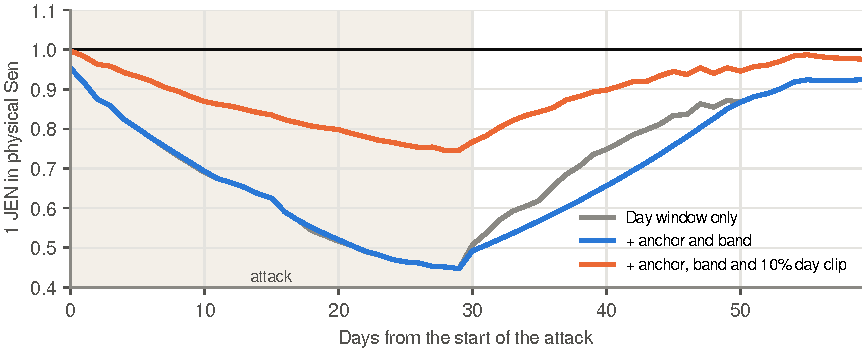
\includegraphics[width=0.92\textwidth]{figs/daywin.pdf}
\caption{A 30-day attack by 10\% of all payments, under three versions of the reading (simulated, \texttt{daywin.js}). The shaded band is the attack.}
\label{fig:daywin}
\end{figure}

Table~\ref{tab:defences} and Figure~\ref{fig:coindays} give the attacker's cost on Jen at one million payments a day, \$2.47M of coin-priced value a day. Normal wander of $S$ is 2--4\%.

\begin{table}[htbp]
\centering\small
\begin{tabularx}{\textwidth}{Y l r r r}
\toprule
\textbf{Defences} & \textbf{Attacker's money} & \textbf{Move 7 d / 30 d} & \textbf{Locked} & \textbf{Lost in 30 d}\\
\midrule
Day window, count-weighted, fees only & fees & 13\% / 31\% & -- & \$3k / \$10k\\
Full set (each gram once, value weighting, cap, bond) & \$1M & 13\% / 16\% & \$2.2M & \$27k\\
Full set & \$5M & 11\% / 20\% & \$11M & \$177k\\
+ coin-days & \$1M & 6\% / 6\% & \$1.2M & \$10k\\
+ coin-days & \$5M & 13\% / 19\% & \$6.4M & \$42k\\
+ bond penalty & \$1M & 12\% / 17\% & \$2.3M & \$417k\\
+ coin-days + bond penalty & \$1M & 4\% / 6\% & \$1.2M & \$116k\\
+ coin-days + bond penalty & \$5M & 12\% / 18\% & \$6.2M & \$534k\\
+ coin-days + bond penalty & \$25M & 13\% / 23\% & \$30M & \$2.7M\\
\bottomrule
\end{tabularx}
\caption{Largest move of $S$ for the attacker's best strategy, money locked (attacker's money and bonds) and money lost in 30 days (fees, 5\% a year interest and burned penalties). Jen at one million payments a day (simulated, \texttt{volsim2.js}, specification 6.6).}
\label{tab:defences}
\end{table}

\begin{figure}[htbp]
\centering
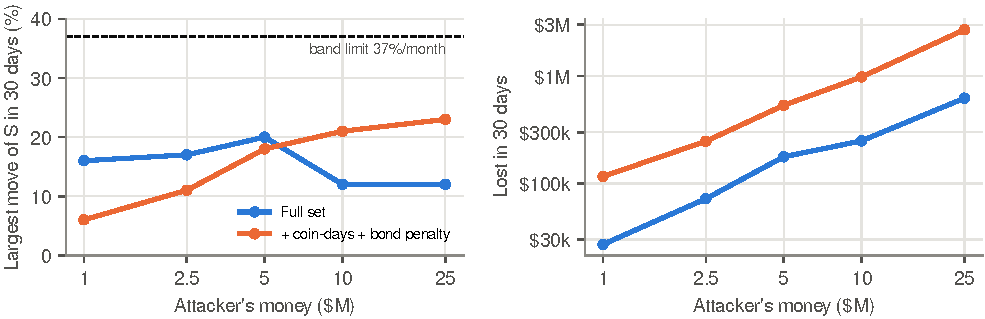
\includegraphics[width=\textwidth]{figs/coindays.pdf}
\caption{Left: the largest 30-day move of $S$ against the attacker's money. Right: what the attack costs him in 30 days. Coin-days and the bond penalty cut what small attackers achieve and multiply what every attacker loses (simulated, \texttt{volsim2.js}).}
\label{fig:coindays}
\end{figure}

\subsection{Watchers and defenders}
The disagreement signal is public, so anyone can run a \emph{watcher}: it shows when the reading leaves the median receiver, in which direction, and which new bonded accounts move together. Watchers decide nothing on the chain; they warn wallets (``peg under pressure: settle at the 30-day average'') and let \emph{defenders} act. A defender (shops, exchanges, a community fund) adds real payments at the honest typical price from rested money. Its payments agree with the median, so it pays no penalty and cannot push $S$ past the truth. Half the attacker's money is enough, because the defender strengthens the honest middle that the reading already favours (Figure~\ref{fig:defender}, Table~\ref{tab:defender}).

\begin{figure}[htbp]
\centering
\begin{minipage}[c]{0.5\textwidth}\centering
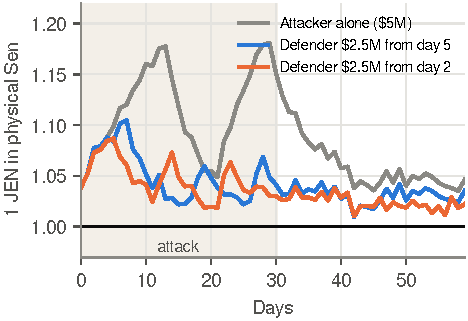
\includegraphics[width=\textwidth]{figs/defender.pdf}
\end{minipage}\hfill
\begin{minipage}[c]{0.47\textwidth}
\caption{A \$5M attacker with all defences, alone and against a defender with half his money joining after 2 or 5 days (simulated, \texttt{defend.js}). The defender brings $S$ back under 5\% within days, at about a twentieth of the attacker's cost.}
\label{fig:defender}
\end{minipage}
\end{figure}

\begin{table}[htbp]
\centering\small
\begin{tabular}{l l l r r r r}
\toprule
\textbf{Attacker} & \textbf{Defender} & \textbf{Joins} & \textbf{Peak} & \textbf{Under 5\% by} & \textbf{Defender spends} & \textbf{Attacker spends}\\
\midrule
\$5M (alone 18\%) & \$2.5M & day 2 & 9\% & day 8 & \$24k & \$534k\\
\$5M & \$2.5M & day 5 & 10\% & day 11 & \$21k & \$534k\\
\$5M & \$5M & day 2 & 6\% & day 7 & \$48k & \$534k\\
\$25M (alone 23\%) & \$12.5M & day 2 & 8\% & day 4 & \$119k & \$2.7M\\
\$25M & \$12.5M & day 5 & 11\% & day 10 & \$106k & \$2.7M\\
\bottomrule
\end{tabular}
\caption{Attacker against defender over 30 days (simulated, \texttt{defend.js}).}
\label{tab:defender}
\end{table}

\subsection{The exchange as a second and third reading}\label{sec:exreading}
Once Ken and Yen exist, every trade between the chains is also a payment on each chain. Some traders quote in coins (``1 \KEN{} for 212 \JEN'', from the metal prices). These coin-priced trades are the exchange's version of coin-priced shop payments. From the day's batch auctions, each chain gets two more readings of its weight:
\begin{equation}
S_{\text{Jen}}^{(\text{Jen--Ken})} = S_{\text{Ken}} \times \frac{\text{Ken grams per Jen gram}}{\text{Jen coins per Ken coin}},
\end{equation}
and likewise from Jen--Yen. The day's value for each chain is the \textbf{median of three}: its own payments and the two exchange readings \st{Proposed, simulated}. An attacker must win two of the three. Exchange readings are hard to fake: the order book is open and every trade in a batch clears at one price, so an order at a wrong coin ratio is filled by others, who profit from it.

\begin{figure}[htbp]
\centering
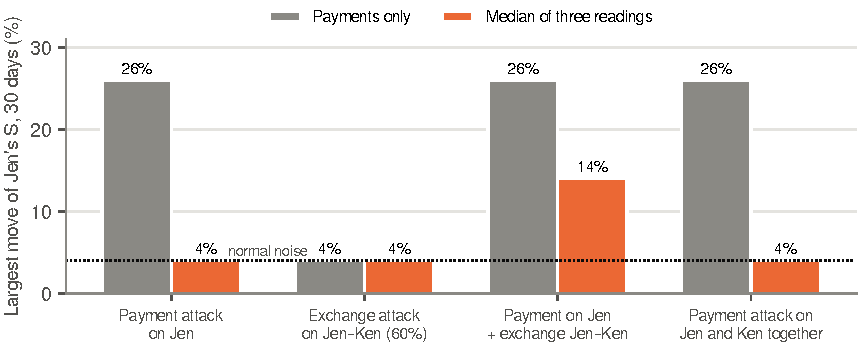
\includegraphics[width=0.92\textwidth]{figs/exchange.pdf}
\caption{Largest 30-day move of Jen's $S$ with and without the exchange readings (simulated, \texttt{tri2.js}). A payment attack on one or two chains is held to normal noise; moving Jen requires also holding the exchange.}
\label{fig:exchange}
\end{figure}

With \$5M a day of coin-priced Jen--Ken trading, holding 60\% of it at 13\% off the true ratio loses the attacker about \$1M a day to the traders who fill him: about \$30M a month for a 14\% move (Figure~\ref{fig:exchange}). The same comparison doubles as a \textbf{counterfeit detector}: when one chain's payment reading departs from both of its exchange readings while the other chains stay normal, trust in that chain's physical coin has changed, for example through counterfeit Ren. The median keeps the electronic coin at its metal value meanwhile, and the community checks the physical coins (weight, size, conductivity, assay).

\subsection{What an attack costs}
Figure~\ref{fig:costs} summarizes the layers. A 12\% push held for a month on Jen at one million payments a day costs about \$3k in fees with no defences; about \$45k a month and \$1.9M locked with each gram once, the cap and the bond; about \$0.5M a month and \$6M locked with coin-days and the penalty; and about \$30M a month once Ken and Yen trade. The simulations assume the attacker already holds the coins. He cannot print them: he must mine or mint them, buy them (raising their price, and holders of money that keeps its value are reluctant to sell it for weaker money, Thiers' law), turn metal into them, or borrow them, and borrowed coins arrive fresh with no coin-days. Every defence is paid in Zen, so security grows with adoption, as Bitcoin's hash rate makes a 51\% attack harder as it grows. The weakest period is the start, when the largest holders are the first miners and minters, who also have the most to lose if the peg breaks.

\begin{figure}[htbp]
\centering
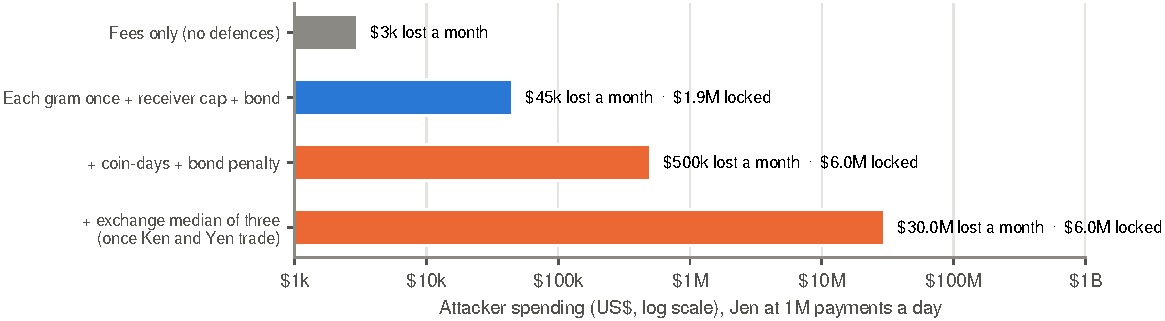
\includegraphics[width=\textwidth]{figs/costs.pdf}
\caption{Cost of holding a 12\% push on Jen's $S$ for a month, by defence level (simulated; log scale). Each layer multiplies the cost roughly tenfold.}
\label{fig:costs}
\end{figure}

\begin{table}[htbp]
\centering\small
\begin{tabularx}{\textwidth}{l Y Y}
\toprule
\textbf{Layer} & \textbf{Rule} & \textbf{What it stops}\\
\midrule
Reading & $S$ = typical ordinary value $\div$ typical coin-priced price; exact sixths & --\\
Each gram once & rested, fresh and used balances; 3-day rest & paying oneself in a loop\\
Value and coin-days & weight = value $\times\min(\text{age},30)/30$ & cycled and borrowed money\\
Window, clip, anchor, band & Fibonacci days; 10\% clip; 2.9\%/day anchor; $\pm10\%$ band & any attack beyond $\approx$13\%/week, 37\%/month\\
Receivers & 0.03\% cap; 7-day bond, +20\%/day on disagreement; 2\%/day penalty & concentrated and spread-thin attackers\\
Freeze & a disagreement day does not count & fast, large pushes\\
Exchange & median of payments and two exchange pairs & payment attacks on one or two chains\\
Settlement & contracts and conversions at the 30-day average & profiting from short pushes\\
Fee limits in coins & smallest fee 0.01 coin; smallest payment $=$ smallest fee $\div$ top rate & a floor that rises with large payments\\
\bottomrule
\end{tabularx}
\caption{The peg defences in layers (specification 6.9).}
\label{tab:layers}
\end{table}

\subsection{When does one \JEN{} become one \SEN?}\label{sec:converge}
At launch $S$ is a genesis guess and must move to the true value from honest payments. Shops that price from the physical coin pull $S$ to the truth; shops that convert from the network's own rate report $S$ back to itself. Figure~\ref{fig:converge} and Table~\ref{tab:converge} show the result: with at least 70\% of coin-priced value set from the physical coin, 1~\JEN{} is within 5\% of 1~\SEN{} in 20 to 57 days, from a start anywhere between a third and three times the truth. At 50\% it takes up to about 100 days; at 30\% it can stall for more than a year.

\begin{figure}[htbp]
\centering
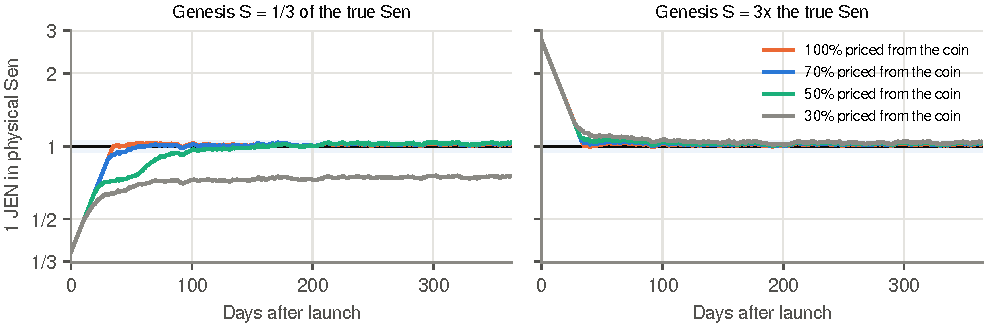
\includegraphics[width=\textwidth]{figs/converge.pdf}
\caption{Convergence of the peg from a wrong genesis weight, by the share of coin-priced value whose price is set from the physical coin. The blue band is $\pm5\%$ (simulated, \texttt{volsim.js}, anchor and band from day 1).}
\label{fig:converge}
\end{figure}

\begin{table}[htbp]
\centering\small
\begin{tabular}{l r r r r}
\toprule
\textbf{Share priced from the physical coin} & \textbf{$S$ starts at $\tfrac13$} & \textbf{$\tfrac12$} & \textbf{$2\times$} & \textbf{$3\times$}\\
\midrule
90--100\% & 34 & 20 & 20 & 34\\
70\% & 46 & 21 & 20 & 57\\
50\% & 98 & 27 & 75 & 84\\
30\% & $>$365 (stuck near 0.75) & 303 & 321 & 321\\
\bottomrule
\end{tabular}
\caption{Days until 1~\JEN{} stays within 5\% of 1~\SEN{} (simulated, \texttt{converge.js}). A 30-day launch phase without anchor and band shortens this to 0--22 days at 70\% or more, but leaves the launch unprotected.}
\label{tab:converge}
\end{table}

The lesson is practical as much as technical: wallets should quote coin prices and coin ratios from metal prices by default, not from the network's $S$. A reading taken from payments can feed on itself once prices are set from it, as the authors of UTXOracle note for their own estimator \cite{utxoracle}.

%=====================================================================
\FloatBarrier
\section{Three currencies, six coins: a self-correcting system}\label{sec:selfcorrect}

Sections~\ref{sec:pom}--\ref{sec:peg} describe the machinery. This section states the thesis behind it: physical money and electronic money each fail in ways the other does not, a single currency is easy to attack, and three linked currencies, each tied to a physical coin, form a system that measures itself, points to where it is being attacked, and pulls itself back. The thesis is stated as a proposal; Section~\ref{sec:sclimits} says where it holds and where it does not.

\subsection{Two kinds of money, complementary failures}

\begin{table}[htbp]
\centering\small
\begin{tabularx}{\textwidth}{l Y Y Y}
\toprule
\textbf{Problem} & \textbf{Physical metal alone} & \textbf{Cryptocurrency alone} & \textbf{Zen (both, linked)}\\
\midrule
Safe storage & needs a vault or trusted custodian; theft & keys on a phone; no vault & savings can sit in either form; neither needs a custodian\\
Long-distance payment & slow, costly, risky to ship & instant & paid electronically; metal stays home\\
Counterfeiting & fake coins, hard to test & impossible (signatures) & counterfeit physical coins show up as a divergence in the readings (Section~\ref{sec:exreading})\\
Volatility & value of the metal only & large swings & electronic coin tracks a fixed metal weight\\
Forks and thousands of coins & -- & value split across chains and copies & one design, three metals, each with a physical anchor that a copy cannot take with it\\
Small daily payments & small coins cost more to mint than they are worth & fees and block space & Jen in sixths of a Sen; channels below that\\
Single point of attack & one metal, one market & one chain, one price & three chains and three cross rates that check each other\\
\bottomrule
\end{tabularx}
\caption{What each kind of money lacks, and how Zen combines them.}
\label{tab:complement}
\end{table}

\subsection{Why three, and not one or two}
With $n$ linked currencies there are $n(n-1)/2$ exchange rates. With \textbf{one} currency there is no rate at all: nothing inside the system can say its value has been pushed. With \textbf{two} there is one rate. If that rate departs from the ratio of the two metals, something is wrong, but the system cannot say which side moved: a push on Jen and a push on Ken in the other direction look identical. With \textbf{three} there are three rates, of which two are independent, and the attacked currency becomes identifiable.

Let $x_i$ be the log deviation of chain $i$'s electronic coin from its physical coin (zero when $1~\JEN=1~\SEN$). Each electronic cross rate, compared with the ratio of the metals in the two physical coins, gives a residual
\begin{equation}
r_{ij} = x_i - x_j \qquad (\text{e.g. } r_{\text{Jen,Ken}} = \log\frac{\text{Jen coins per Ken coin on the exchange}}{\text{Sen per Ten from metal prices}}).
\end{equation}
An attack on Jen moves $r_{\text{Jen,Ken}}$ and $r_{\text{Jen,Yen}}$ together and leaves $r_{\text{Ken,Yen}}$ flat: the odd one out is named. This is the logic of triple modular redundancy and of $2f+1$ fault tolerance with $f=1$: three members can identify one faulty member. Triangular arbitrage keeps the three electronic rates consistent with each other ($\tfrac{J}{K}\cdot\tfrac{K}{Y}\cdot\tfrac{Y}{J}=1$) whatever happens, so the signal is not in the triangle closing; it is in each rate against its metal ratio.

\paragraph{Everything is public, in grams.} The triangle of cross rates is only what an outside observer sees. Inside Zen there is much more, and all of it is public. Each chain publishes its coin weight $S$, the grams of its money that make one coin, in every block. Every trade between the chains settles on-chain, so the gram rate of each pair is public. And coin-priced trades (``1~\KEN{} for 212~\JEN'') carry the coin ratio that traders take from the metal markets. Together these give every chain three readings of what its physical coin is worth (Section~\ref{sec:exreading}): its own coin-priced payments, and one reading through each of its two exchange pairs, built from the partner chain's public weight, the pair's gram rate and the coin ratio:
\begin{equation}
I_{\text{Jen}}^{(\text{Ken})} = S_{\text{Ken}}\times\frac{\text{Ken grams per Jen gram}}{\text{Jen coins per Ken coin}} .
\end{equation}
That is nine public readings, recomputed by every node and every wallet from the blocks and the batch auctions, with no oracle. An attacker can bias six things: the payments of each chain, and the coin-priced orders of each pair. Each leaves its own fingerprint. Fake payments on Jen move one reading, Jen's own, and leave Jen's two exchange readings in agreement against it. Wrong-ratio orders on Jen--Ken move two readings in opposite directions, Jen's reading through Ken and Ken's reading through Jen, while both chains' payments disagree with them. Because every reading is redundant, the smallest set of biased components that explains all nine is the attack, and it is unique for any attack on one or two components.

\begin{figure}[htbp]
\centering
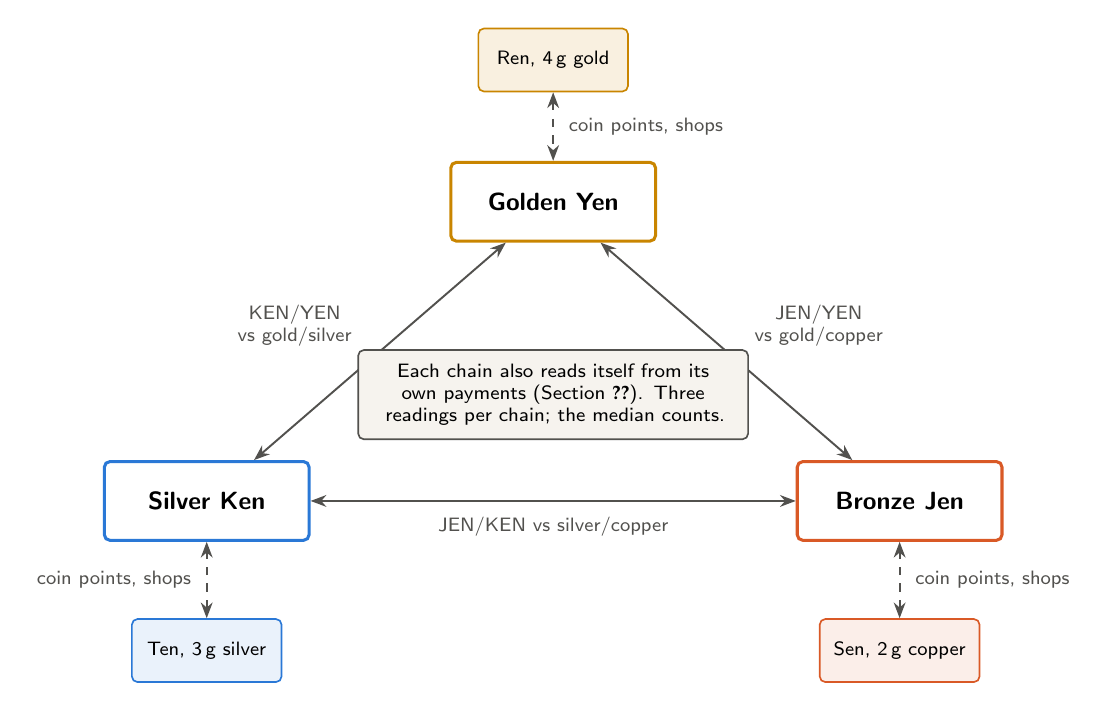
\begin{tikzpicture}[
  ch/.style={box,line width=1.1pt,minimum width=2.6cm,minimum height=1.0cm},
  ph/.style={box,minimum width=1.9cm,minimum height=0.8cm,font=\sffamily\scriptsize}]
  \node[ch,draw=yen] (Y) at (0,3.8) {\textbf{Golden Yen}};
  \node[ch,draw=ken] (K) at (-4.4,0) {\textbf{Silver Ken}};
  \node[ch,draw=jen] (J) at (4.4,0) {\textbf{Bronze Jen}};
  \draw[arr,{Stealth[length=2mm]}-{Stealth[length=2mm]}] (Y) -- node[lbl,above left=2pt and 2pt,pos=0.55] {KEN/YEN\\vs gold/silver} (K);
  \draw[arr,{Stealth[length=2mm]}-{Stealth[length=2mm]}] (Y) -- node[lbl,above right=2pt and 2pt,pos=0.55] {JEN/YEN\\vs gold/copper} (J);
  \draw[arr,{Stealth[length=2mm]}-{Stealth[length=2mm]}] (K) -- node[lbl,below=2pt] {JEN/KEN vs silver/copper} (J);
  \node[ph,fill=yen!12,draw=yen] (R) at (0,5.6) {Ren, 4\,g gold};
  \node[ph,fill=ken!10,draw=ken] (T) at (-4.4,-1.9) {Ten, 3\,g silver};
  \node[ph,fill=jen!10,draw=jen] (Sn) at (4.4,-1.9) {Sen, 2\,g copper};
  \draw[arr,dashed,{Stealth[length=2mm]}-{Stealth[length=2mm]}] (R) -- node[lbl,right=2pt] {coin points, shops} (Y);
  \draw[arr,dashed,{Stealth[length=2mm]}-{Stealth[length=2mm]}] (T) -- node[lbl,left=2pt] {coin points, shops} (K);
  \draw[arr,dashed,{Stealth[length=2mm]}-{Stealth[length=2mm]}] (Sn) -- node[lbl,right=2pt] {coin points, shops} (J);
  \node[box,fill=wash,text width=4.6cm,font=\sffamily\scriptsize] at (0,1.35) {Each chain also reads itself from its own payments (Section~\ref{sec:peg}). Three readings per chain; the median counts.};
\end{tikzpicture}
\caption{Six coins, three cross rates. Each electronic cross rate is checked against the ratio of the metals; each electronic coin is also traded against its own physical coin at coin points and in shops. An attack on one chain bends two sides of the triangle and leaves the third straight.}
\label{fig:triangle}
\end{figure}

\subsection{Reading the signals}
Because every chain has three readings (its own payments and two exchange pairs, Section~\ref{sec:exreading}) and the world has independent markets for the three metals, distinct events leave distinct patterns:

\begin{table}[htbp]
\centering\small
\begin{tabularx}{\textwidth}{Y Y Y}
\toprule
\textbf{Pattern} & \textbf{Likely cause} & \textbf{What corrects it}\\
\midrule
One chain's two cross residuals move together; the third stays flat & attack on that chain's peg & median of three holds $S$; arbitrage and defenders push back\\
One chain's payment reading departs from both of its exchange readings; cross residuals normal & trust in that chain's \emph{physical} coin has changed (counterfeits) & median keeps the electronic coin at metal value; physical testing\\
All three move together against metal prices; cross residuals flat & common shock: demand for Zen as a whole, or a general metal move & nothing to correct; $S$ follows at the anchor's pace\\
Two chains' payment readings each depart from their own exchange readings & payment attack on both chains & each chain's median holds; both are named\\
One pair's two readings move in opposite directions & wrong-ratio orders on that pair (exchange attack) & the attacker's orders are filled by others at a loss\\
All three readings of one chain move together & a real move of that metal, or an attacker holding the chain's payments and both its pairs at once & the anchor follows at 2.9\% a day; world metal prices tell which (Section~\ref{sec:sclimits})\\
\bottomrule
\end{tabularx}
\caption{Signals and their likely causes.}
\label{tab:signals}
\end{table}

\subsection{The correcting forces}
Detection is useful only if something pulls the system back. Four forces do, none of them a central party:
\begin{enumerate}
\item \textbf{The protocol.} Each chain's day value is the median of three readings, and $S$ moves at most 2.9\% a day within a $\pm10\%$ band (Section~\ref{sec:defences}). A pushed reading is outvoted or held.
\item \textbf{Triangular arbitrage.} If the three electronic rates disagree with each other, traders profit by cycling through them until they agree.
\item \textbf{Coin-for-coin arbitrage.} Where an electronic coin buys more or less than its physical coin (at stream nodes that act as coin points, Section~\ref{sec:channels}, or in shops that accept both), traders buy the cheap form and sell the dear one, pulling the two together.
\item \textbf{Defenders.} Because the signal is public and attributes the attack, shops, exchanges and community funds know where to add honest payments; in simulation half the attacker's money undoes the push at about a twentieth of his cost (Section~\ref{sec:defences}).
\end{enumerate}

\subsection{How fast an attack is seen}
A model of the nine readings makes the claim concrete \st{simulated}. Every hour, each chain's payment reading has noise of about 5\% (1\% a day) and each exchange reading about 3\% (0.67\% a day), the same noise as in the three-chain peg model (\texttt{tri2.js}); thin, young markets get three times as much. A detector, which any node or wallet can run on the public data, fits the readings over the last 1 to 24 hours with the smallest set of biased components; it raises an alarm when some set explains the readings much better than none, with the threshold set for about one false alarm in five quiet years. The day after the alarm it names the components. An attacker pushes his readings by 2\% to 25\%; 25\% is roughly what the \$5M attacker of Table~\ref{tab:defences} achieves on Jen's payment reading.

\begin{figure}[htbp]
\centering
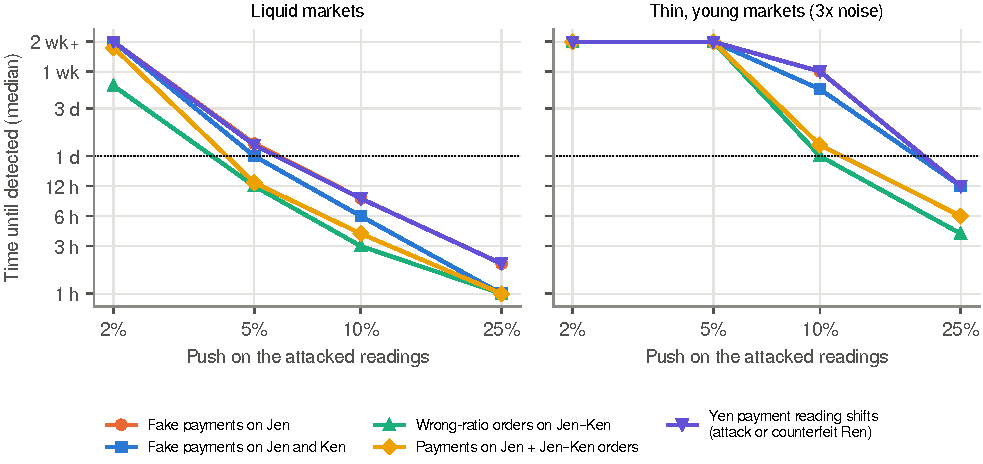
\includegraphics[width=\textwidth]{figs/detect9.pdf}
\caption{Time until an attack is detected from the nine public readings, by attack type and size (median of 400 runs per point; simulated, \texttt{detect9.py}). Fake payments on Jen and a shift of Yen's payment reading behave identically and overlap. ``2 wk+'' means not detected within 14 days.}
\label{fig:detect9}
\end{figure}

\begin{table}[htbp]
\centering\small
\begin{tabularx}{\textwidth}{Y r r r r r r}
\toprule
& \multicolumn{3}{c}{\textbf{Liquid markets}} & \multicolumn{3}{c}{\textbf{Thin markets}}\\
\cmidrule(lr){2-4}\cmidrule(lr){5-7}
\textbf{Attack} & \textbf{5\%} & \textbf{10\%} & \textbf{25\%} & \textbf{5\%} & \textbf{10\%} & \textbf{25\%}\\
\midrule
Fake payments on Jen & 32 h & 9 h & 2 h & -- & 7 d & 12 h\\
Fake payments on Jen and Ken & 24 h & 6 h & 1 h & -- & 5 d & 12 h\\
Wrong-ratio orders on Jen--Ken & 12 h & 3 h & 1 h & -- & 24 h & 4 h\\
Payments on Jen + Jen--Ken orders & 13 h & 4 h & 1 h & -- & 31 h & 6 h\\
Yen payment reading shifts (attack or counterfeit Ren) & 31 h & 9 h & 2 h & -- & 7 d & 12 h\\
\midrule
\textit{Right components named, within a day of the alarm} & 99--100\% & 99--100\% & 99--100\% & -- & 74--100\% & 99--100\%\\
\bottomrule
\end{tabularx}
\caption{Median time to detection from the nine public readings (simulated, \texttt{detect9.py}). ``--'': not detected within 14 days, because a 5\% push in thin markets stays inside normal noise. A 2\% push is not detected in either case; it is within the normal 2--4\% wander of $S$.}
\label{tab:detect9}
\end{table}

Three results stand out. First, an attack of the size that matters is seen within hours: a 25\% push on the readings within one or two hours in liquid markets, and within half a day in thin ones. $S$ changes only when a day's reading closes, and then within the day clip and the anchor's band, so the alarm comes before the attacked day has even been counted. Second, the attack is \emph{named}, not only seen, in 99--100\% of runs once it is above the noise, including attacks on two chains at once and combinations of payments and exchange orders. Third, pushes smaller than the normal wander are not detected, and need not be: they are smaller than the error the peg already tolerates.

Because the chains are public, the alarm also points to the accounts. Payments that count toward $S$ come from accounts with rested balances and bonded receivers (Section~\ref{sec:defences}), so watchers can list which new bonded receivers moved together, where their money came from, and when it arrived. The same data separates an attack from a counterfeit wave: fake payments on Yen come from a few recently bonded accounts with concentrated value, while a loss of trust in physical Ren shifts the prices of many long-established shops at once.

\subsection{One money for the user}
To a user, Zen can look like one currency in three sizes, as gold, silver and copper once were. A wallet holds all three and shows a single balance in the unit its owner chooses (for example Sen, or the local currency at today's metal prices); it pays large amounts in Yen, everyday amounts in Ken or Jen and fractions in Jen over channels, swapping between them through stream nodes in the same atomic payment (Section~\ref{sec:channels}). Unlike historical trimetallism, the ratios between the three are not fixed by law but float with the metal markets, so Gresham's law has no fixed ratio to exploit. The cost of that freedom is that a balance shown in one unit moves when the metal ratios move; the gold--silver ratio, for instance, changes over years.

\subsection{Where the thesis holds and where it does not}\label{sec:sclimits}
\begin{itemize}
\item \textbf{``Instantly detectable''} holds in a practical sense: every node can compute all nine readings from public data every block, and attacks large enough to matter are named within hours. Small pushes take days, or stay hidden inside normal noise, where they do no harm.
\item \textbf{One chain fully held.} An attacker who controls a chain's payments \emph{and} both of its exchange pairs moves all three of its readings together. That looks exactly like a genuine move of that metal. Zen's answer is the anchor, which lets $S$ follow any such move at no more than 2.9\% a day, and the world metal prices, which anyone can compare: if copper did not move, the attack is visible. Holding Jen's payments and two exchange pairs costs on the order of \$60M a month at one million payments a day (Section~\ref{sec:exreading}).
\item \textbf{Common shocks are invisible by design.} If demand for all of Zen rises or falls, or all metals move together, all nine readings stay consistent. That is correct behaviour: there is nothing to correct.
\item \textbf{Correction needs liquidity and honest pricing.} Arbitrage only works where the exchange and coin points have volume, detection in thin markets takes days instead of hours, and the peg converges only if most coin-priced shops price from the metal (Section~\ref{sec:converge}). Before Ken and Yen exist, Jen has its payments and its coin-for-coin market only.
\item \textbf{Metal prices enter through people.} No metal price is in consensus. The metal ratios enter the readings through the coin ratios traders quote, and through the shops that price in coins; watchers can compare everything with world metal prices, but the chains do not.
\end{itemize}

%=====================================================================
\FloatBarrier
\section{Channels and channel factories (L2)}\label{sec:channels}

On-chain capacity is finite and every payment is public. Zen moves most small payments into channels: coins are \emph{melted} into a channel, \emph{streamed} off-chain and \emph{cast} back on-chain \st{Decided}.

\begin{table}[htbp]
\centering\small
\begin{tabularx}{\textwidth}{l l Y}
\toprule
\textbf{Step} & \textbf{On-chain?} & \textbf{Mechanism}\\
\midrule
Melt & yes & funds enter a channel or factory (funding transaction)\\
Stream & no & balance updates signed by both sides; only the latest state counts (eltoo-style, built in from launch)\\
Cast & yes, final balances only & closing transaction; one member may leave a factory without closing it for the others\\
\bottomrule
\end{tabularx}
\caption{The channel life cycle (specification 7.1).}
\end{table}

\paragraph{Channel types.} Two-party channels carry routed payments; one-way streams pay per second or per use with minimal state (the payer signs increasing balances, with no revocation state); and \emph{channel factories} put many users behind one on-chain output, with a coordinating stream node keeping them live when members are offline.

\paragraph{Routing across metals.} Payments hop through stream nodes inside onion encryption, so each node knows only its neighbours. Every hop is locked with a point lock (PTLC), the same lock family on all three chains, so a route such as Jen $\to$ Ken $\to$ Yen completes on every chain or on none. Blinded routes hide the receiver. A stream node with channels on two metals receives one and sends the other, earning a routing fee plus an exchange spread, and can act as a physical-coin point that checks a Ren, Ten or Sen by hand and streams the same value.

\paragraph{Privacy.} The chain stays fully public, which keeps purity, the coin weight and exchange rates measurable. Privacy comes from the channel layer: off-chain payments, onion routing, point locks and blinded routes. There is no shielded pool on layer 1, given the EU AMLR rules from 10 July 2027 that also cover coins with optional privacy \st{Decided}.

\paragraph{Status on the test network.} \st{Testnet} The Rust node runs this layer today on a three-chain test network: two-party and dual-funded channels, one-way streams, point locks inside channel states, onion-routed payments across channels and across chains (a route from Jen through Ken to Yen settled on all three), factories of up to eight members with exit by one member alone, watchtowers fed automatically by the node, and an encrypted, authenticated transport for the off-chain messages. Channel and factory operations are carried by the block proof (Section~\ref{sec:stamp}). Not yet built: splicing, encrypted storage and payment for watchtowers, and wider peer discovery.

\subsection{Factories: what they give and what they cost}
Channel factories cut on-chain cost by about 90\% for 20 users and 100 channels \cite{burchert}; the SuperScalar design puts one provider and up to 127 clients in a single output, with an implementation report on a test network in July 2026 \cite{superscalar}. Bitcoin still lacks the covenant these designs want, and every allocation update needs all members to sign. Zen sets its own consensus, so it can ship the missing pieces from the start.

\begin{table}[htbp]
\centering\small
\begin{tabularx}{\textwidth}{Y Y}
\toprule
\textbf{Advantages} & \textbf{Costs and risks}\\
\midrule
little on-chain space per user & every allocation change needs all members' signatures\\
instant, nearly free payments, not limited by block size & mass exits crowd the chain\\
cheap onboarding for phones & members must be online or use a watchtower\\
liquidity moved inside the group without on-chain transactions & funds are locked; providers become hubs\\
privacy; atomic swaps between Yen, Ken and Jen & channel payments do not reach the peg reading, and channel fees do not pay minters\\
\bottomrule
\end{tabularx}
\caption{Channel factories in Zen (specification 15.1).}
\end{table}

Zen's choices \st{Proposed}: a native template covenant, so one member can exit without forcing the whole factory on-chain; eltoo-style updates, where only the latest state counts and no penalty transactions exist \cite{eltoo}; fee sponsorship and a dispute lane for urgent exits; staggered factory expiries so mass exits spread over many blocks; channel closes, splices and factory exits that report the net value settled, as observations for $S$; and a small on-chain fee on factory opens, rebalances and closes, so minters stay paid as volume moves off-chain.

%=====================================================================
\section{Exchange between Yen, Ken and Jen}\label{sec:exchange}

Nobody owns the exchange. Orders are shared off-chain, trades settle on-chain and set the official rates, and fast trading happens in channels \st{Decided}.

\begin{itemize}
\item \textbf{Placing and cancelling orders}: an order gossip network, off-chain and free.
\item \textbf{Peer-to-peer settlement} (first version): the maker locks the coins being sold on that chain (``5~\YEN{} for 60~\KEN, to my Ken address, until block $H$''); a taker reserves the order with a small deposit, pays on the other chain tagged with the order ID, and claims the locked coins by proving the payment with the other chain's stamp and a Merkle proof. The proof is checked by every node against the other chain's headers, which it follows over the network; the block proof binds a digest of it to the claim and to the claimant's signature but does not check the foreign chain itself (Section~\ref{sec:stamp}). Payments are accepted after about 30 minutes of confirmations (for example 2 Yen, 6 Ken or 12 Jen blocks; TBD).
\item \textbf{Bid auctions} \st{Testnet}: a maker may open an order to bids; a higher bid replaces the waiting one inside a window and the earlier bidder is refunded in the same operation, and the highest bid at the close becomes the taker. \textbf{Batch auctions} \st{Open, later version}: each block, the pair's home chain (the higher metal) clears all orders at one price, which prevents front-running and gives one price per block.
\item \textbf{Official rates}: per pair, the volume-weighted median price of filled trades over a day. With $1~\YEN=1~\REN$, $1~\KEN=1~\TEN$ and $1~\JEN=1~\SEN$, these are also the rates between the physical metals. On the test network the rate is the volume-weighted median of the newest 32 fills and exists only when at least three fills come from two makers and two takers (testnet).
\end{itemize}

The three chains float independently, so no legal ratio exists between the metals for Gresham's law to exploit. Fixed ratios defeated bimetallism in the United States (1792--1873) and the Latin Monetary Union (1865--1878) \cite{velde}; Zen fixes no cross-rate, and its exchange check (Section~\ref{sec:exreading}) only compares ratios against the market.

%=====================================================================
\section{Zen Net: a paid network layer (L3)}\label{sec:zennet}

Zen Net is a network on top of Zen's channels and factories in which every node has a wallet and every service is paid for exactly what it does: carrying packets, routing, storing data and computing \st{Proposed}. To go online, a user funds a wallet, joins a factory and pays as they go, with no account, subscription or identity. Anyone, from a phone to a server, can earn by serving others.

\begin{figure}[htbp]
\centering
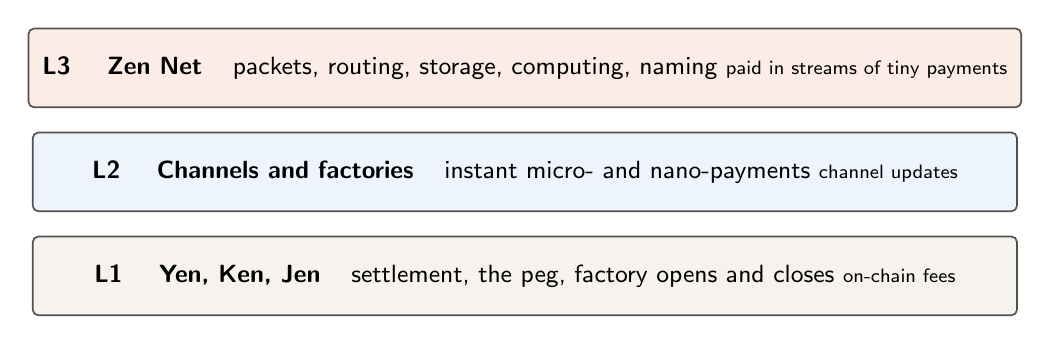
\begin{tikzpicture}
  \node[box,fill=copperwash,minimum width=12.5cm,minimum height=1.0cm,align=left] (l3) {\textbf{L3 \quad Zen Net}\hspace{1.2em}packets, routing, storage, computing, naming \hfill {\scriptsize paid in streams of tiny payments}};
  \node[box,fill=bluewash,minimum width=12.5cm,minimum height=1.0cm,below=3mm of l3,align=left] (l2) {\textbf{L2 \quad Channels and factories}\hspace{1.2em}instant micro- and nano-payments \hfill {\scriptsize channel updates}};
  \node[box,fill=wash,minimum width=12.5cm,minimum height=1.0cm,below=3mm of l2,align=left] (l1) {\textbf{L1 \quad Yen, Ken, Jen}\hspace{1.2em}settlement, the peg, factory opens and closes \hfill {\scriptsize on-chain fees}};
\end{tikzpicture}
\caption{The three layers of Zen.}
\label{fig:layers}
\end{figure}

\paragraph{Paying per packet.} A packet is worth far less than the smallest on-chain payment: 1\,GB at \$0.50 is about 0.001~Sen per 64\,KB, and signing a payment per packet would cost more than forwarding it. Zen Net uses streaming payments (one channel update per chunk, for example every 100\,KB or every second; when payment stops, service stops), probabilistic tickets (a ticket with a 1-in-1,000 chance of paying 1~Sen is worth 0.001~Sen; winners are cashed through channels) and small credit between neighbours settled every few seconds. Prices are quoted in Jen, so they stay stable and readable (``0.3 Sen per MB'').

\begin{table}[htbp]
\centering\small
\begin{tabularx}{\textwidth}{l Y}
\toprule
\textbf{Service} & \textbf{How it is measured and paid}\\
\midrule
Routing and transit & per MB relayed, paid hop by hop\\
Private relays & per MB, through layered tickets that do not reveal who talks to whom\\
Exits and gateways & per MB or per minute, by streaming; an optional role, priced separately\\
Storage & per GB per day, with random challenges proving the data is still held\\
Computing & per job, with a zero-knowledge proof that the result is correct; minters can sell spare proving power\\
Naming and applications & per request, or subscriptions as streams\\
\bottomrule
\end{tabularx}
\caption{Zen Net services (specification 15.3).}
\end{table}

\paragraph{Proof of service.} A router could take payment and drop packets, a storage node delete data, a computer return a wrong result. Payment per acknowledged chunk, relay tickets cashable only after the next hop confirms, storage challenges, zero-knowledge proofs for computing, reputation, and bonded routers (the same bond idea as the peg) make that unprofitable. Related systems include Althea (paid mesh routing), Orchid (probabilistic nanopayments), HOPR and Nym (paid mixnets), Mysterium and Sentinel (VPN markets), Interledger STREAM, and Filecoin, Storj, Arweave, Golem and Akash for storage and computing; these are cited from memory and their status was not verified for this paper. What would be new is one metal-pegged money for every service, factories in the base layer with phones as first-class clients, and computing verified by the same machinery as minting.

%=====================================================================
\section{Upgrades}\label{sec:upgrades}

A change is tested on Jen, confirmed on Ken and only then adopted on Yen, with rising thresholds and time gates \st{Decided}.

\begin{figure}[htbp]
\centering
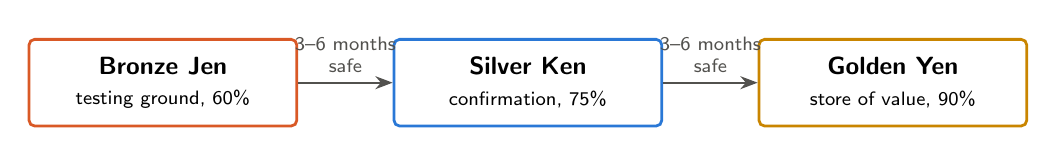
\begin{tikzpicture}[node distance=12mm]
  \node[box,draw=jen,line width=1pt,minimum width=3.4cm,minimum height=1.1cm] (j) {\textbf{Bronze Jen}\\{\scriptsize testing ground, 60\%}};
  \node[box,draw=ken,line width=1pt,minimum width=3.4cm,minimum height=1.1cm,right=of j] (k) {\textbf{Silver Ken}\\{\scriptsize confirmation, 75\%}};
  \node[box,draw=yen,line width=1pt,minimum width=3.4cm,minimum height=1.1cm,right=of k] (y) {\textbf{Golden Yen}\\{\scriptsize store of value, 90\%}};
  \draw[arr] (j) -- node[lbl,above] {3--6 months\\safe} (k);
  \draw[arr] (k) -- node[lbl,above] {3--6 months\\safe} (y);
\end{tikzpicture}
\caption{The upgrade path. Support is measured by work: miners signal in seals and minters in strikes, and both groups must pass the threshold.}
\end{figure}

Thresholds stay above 50\% so activated rules are always enforced by a majority. Every node release validates all three chains under old and new rules before any chain activates, because the chains verify each other's stamps. Critical security fixes ship as software releases without signalling; they never change economic rules.

%=====================================================================
\section{Implementation and devices}\label{sec:impl}

\paragraph{Stack.} One Rust codebase for the node, wallet, minter and miner, built as a desktop app (about 50--100\,MB) and a phone app (about 40--80\,MB), with roles switched on in settings; proving keys (30--120\,MB) download only for minters \st{Decided in principle}. The consensus core uses integer-only arithmetic; zero-knowledge proofs use proven libraries (gnark in the Go prototype; in the Rust benchmark, Plonky2 for leaves and merges and gnark v0.16.4 for the Groth16 stamp, Section~\ref{sec:stamp}); storage is RocksDB, networking libp2p, and the channel code is modelled on LDK. The Rust codebase exists as the \texttt{zenproof} node: three chains on a test network, wallet, pool, explorer, local API, snapshots, encrypted transport, a container image and the proof pipeline of Section~\ref{sec:stamp} (55 numbered build rounds, 137 automated tests, the last full run on 27 October 2026; testnet). Before mainnet: two independent implementations of the consensus core, fuzzing, external audits of circuits and consensus, and a long testnet. Nodes, minters, miners and wallets can connect over the normal internet, Tor or I2P, as Bitcoin Core does; credentials and rewards are tied to keys, never to IP addresses, and every node relays new payments with Dandelion++.

\begin{table}[htbp]
\centering\small
\begin{tabularx}{\textwidth}{l l Y Y}
\toprule
\textbf{Role} & \textbf{Device} & \textbf{Memory} & \textbf{CPU and storage}\\
\midrule
User & any phone & 100--300 MB & 2--4 ms per stamp check (measured); 50--200 MB\\
Minter, phone & phone, $\ge$3 GB RAM & 400--750 MB while proving (measured, 4--8 payments) & seconds per leaf; + 30--60 MB keys\\
Minter, desktop & ordinary PC & 0.9 GB while proving (measured, 16 payments) & 5--6 s per signature leaf on 2 cores (measured)\\
Builder (a pool) & server CPU + NVIDIA GPU & 6 GB for the stamp; 2 GB proving key & 3.7 min per block on 2 cores (measured); target $\approx$60 s\\
Full node & PC, mini PC or small server & 8--16 GB & 4--8 cores; $\approx$10 GB per 100M accounts\\
Stream node & always-on server & 16--32 GB & full node + channel database\\
Miner & SHA-256 ASIC + pool or full node & as full node & Stratum v1, Bitcoin header\\
\bottomrule
\end{tabularx}
\caption{Resources per role (specification 10.2; estimates except where marked measured).}
\end{table}

\paragraph{Phones.} The best minters are the devices people already own. A phone plugged in, on Wi-Fi or 4G/5G, can mint 24 hours a day at about 5 blows a second. On Android the minter ships as an app installed directly (an APK), not through Google Play, whose policy bans on-device mining; it runs as a foreground service, and from September 2026 Google is phasing in developer verification for sideloaded apps (first in Brazil, Indonesia, Singapore and Thailand, globally in 2027), so the app must be signed by a verified developer. On iOS, Apple's App Store rules forbid on-device mining, so iPhones can run the wallet and a light node but not mint; this reflects platform policies as of October 2026.

\paragraph{Computers, mini PCs and Raspberry Pi.} Laptops and desktops mint several times faster than phones, in proportion to their cores, and can take part in merging proofs, which needs about 1\,GB and 4--6.5\,s per merge on 2 cores (measured). The final stamp needs about 6\,GB and a few minutes on 2 cores, less with more cores, so it suits a server. A mini PC is a good always-on full node and merger. A Raspberry Pi with 8\,GB suits a full node, a stream node or a slow minter.

\subsection{The Jen v1 interface}
A first interface for Jen gathers the four things a participant does: transact, mint, mine and watch the coin weight (Figure~\ref{fig:ui}). It is a prototype with sample data, not yet connected to a node. Ken and Yen appear greyed out until they launch.

\begin{figure}[tbp]
\centering
\begin{subfigure}{\textwidth}\centering
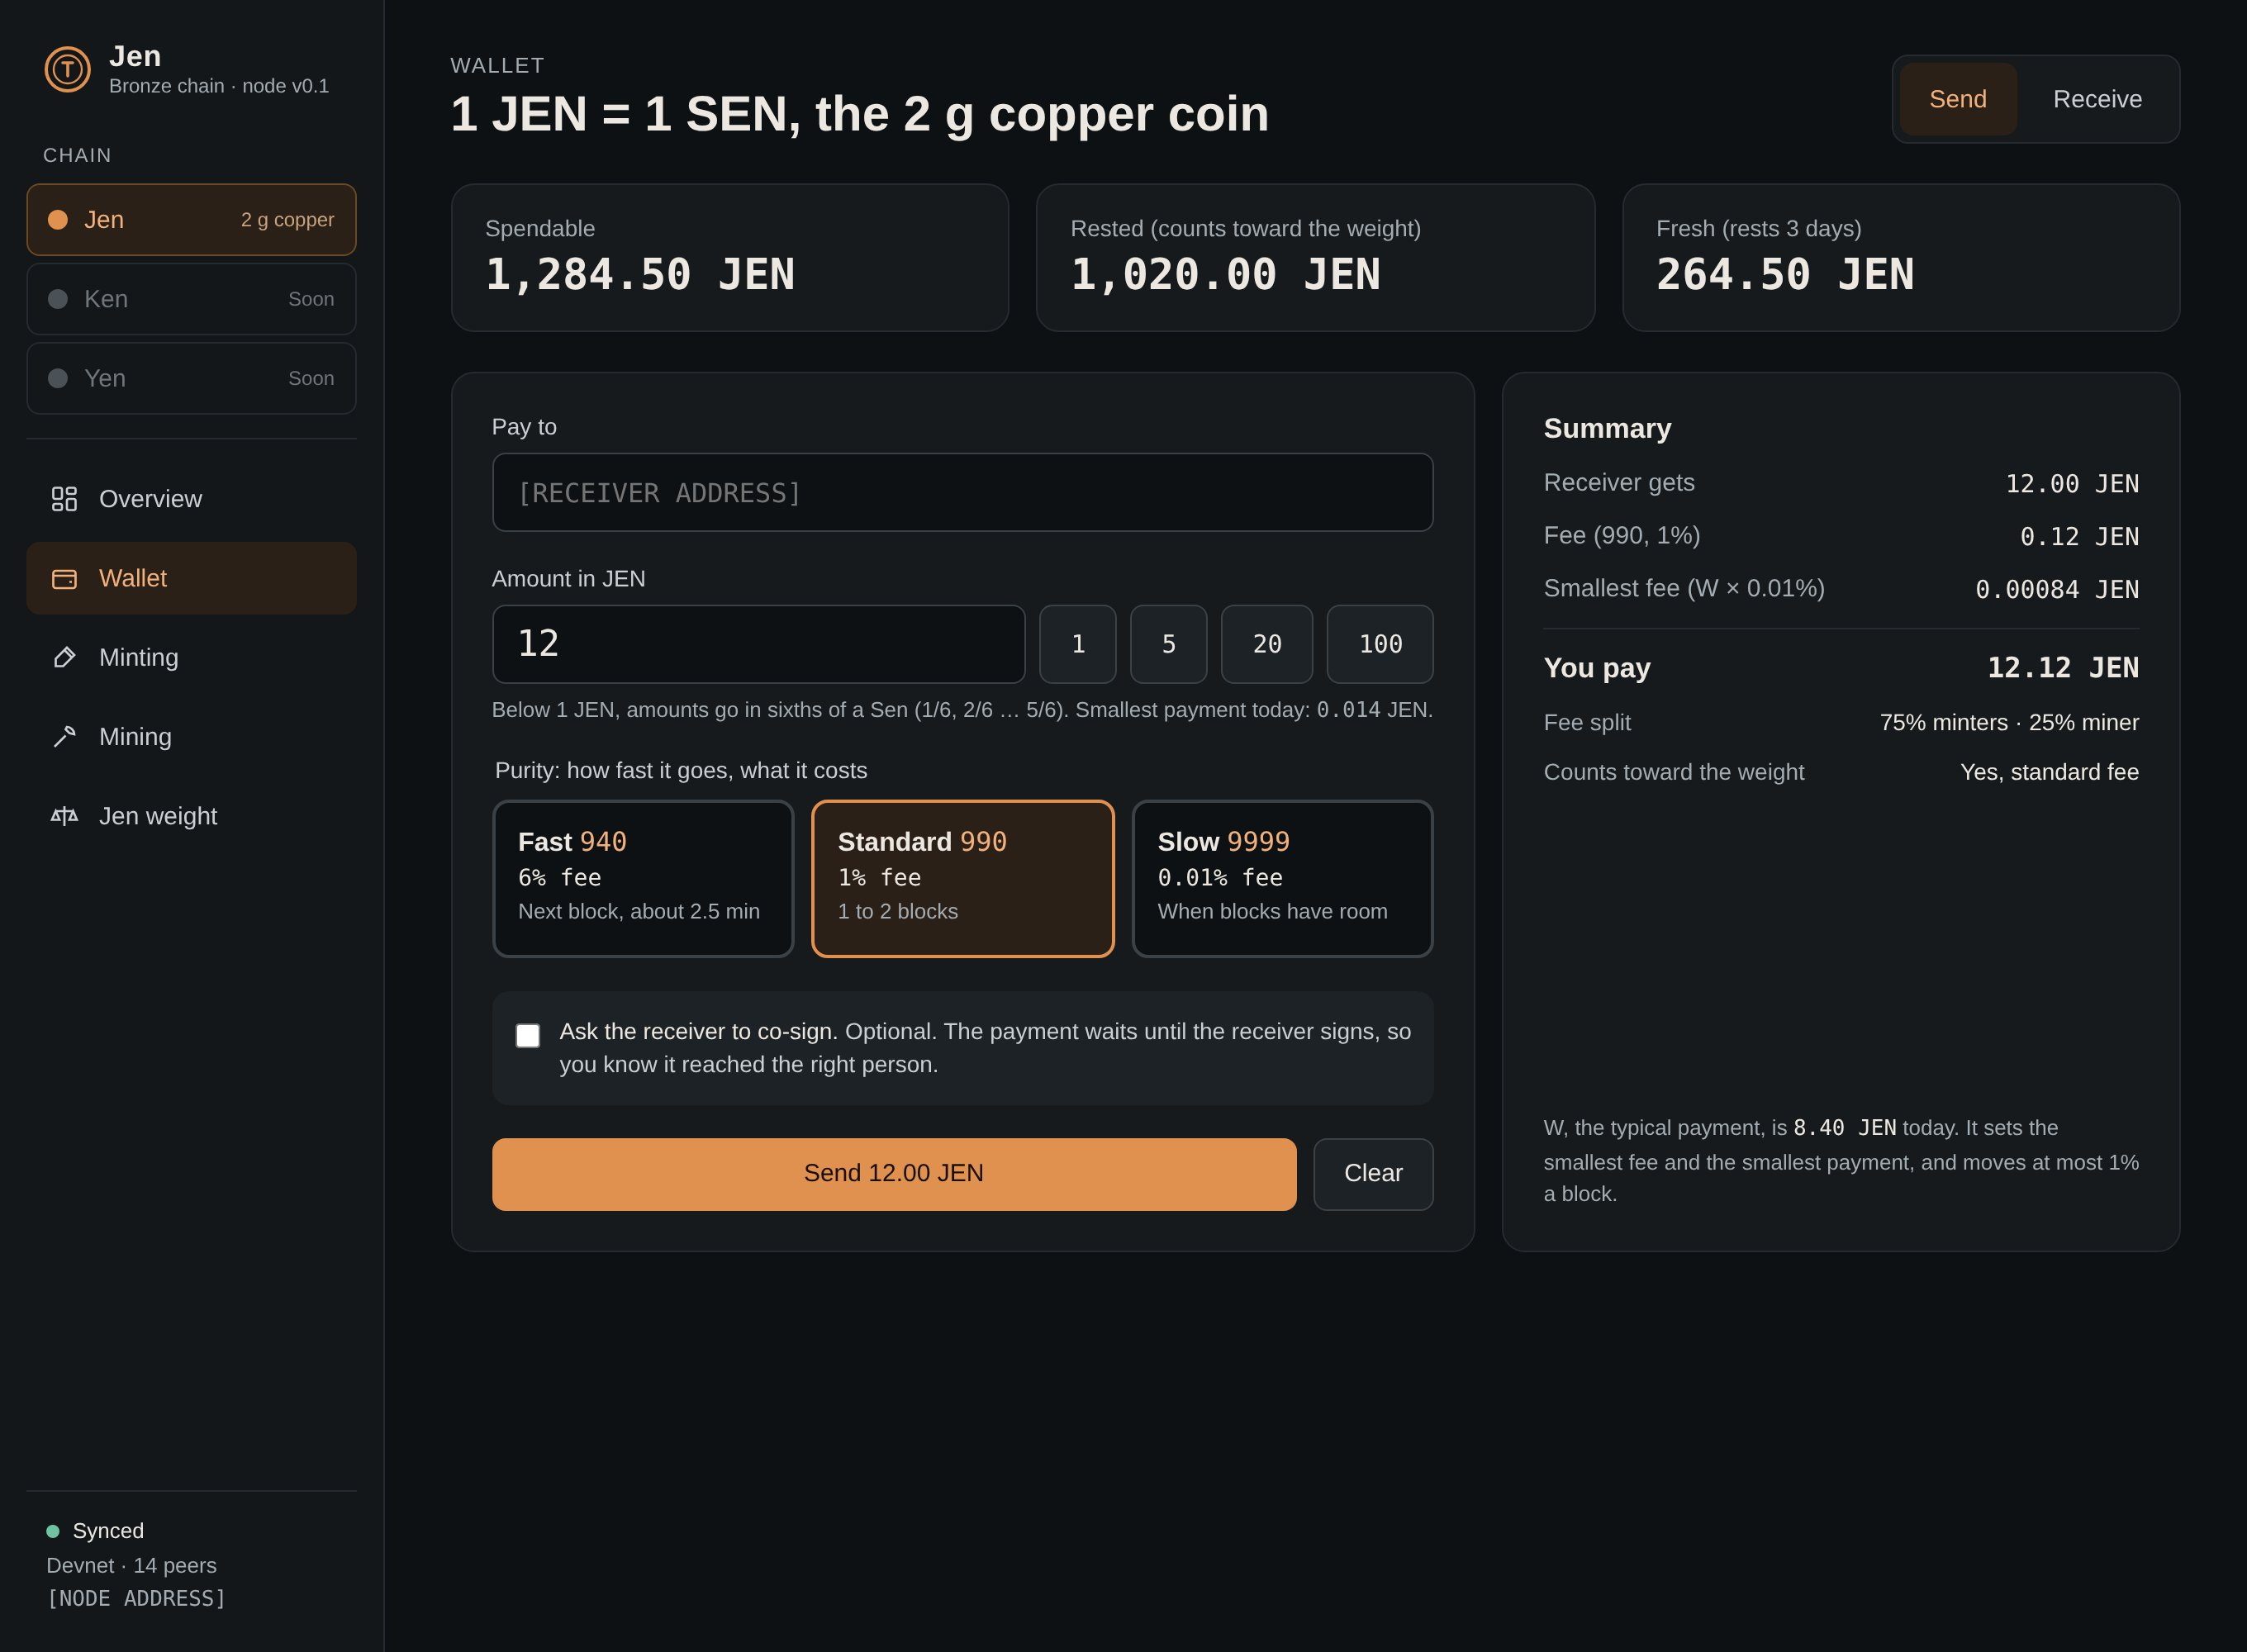
\includegraphics[width=0.98\textwidth]{figs/ui_wallet.jpg}
\caption{Wallet: amount in \JEN{} (sixths below 1), purity choice, optional receiver co-signature, and the fee worked out from the purity and the amount.}
\end{subfigure}\\[8pt]
\begin{subfigure}{0.70\textwidth}\centering
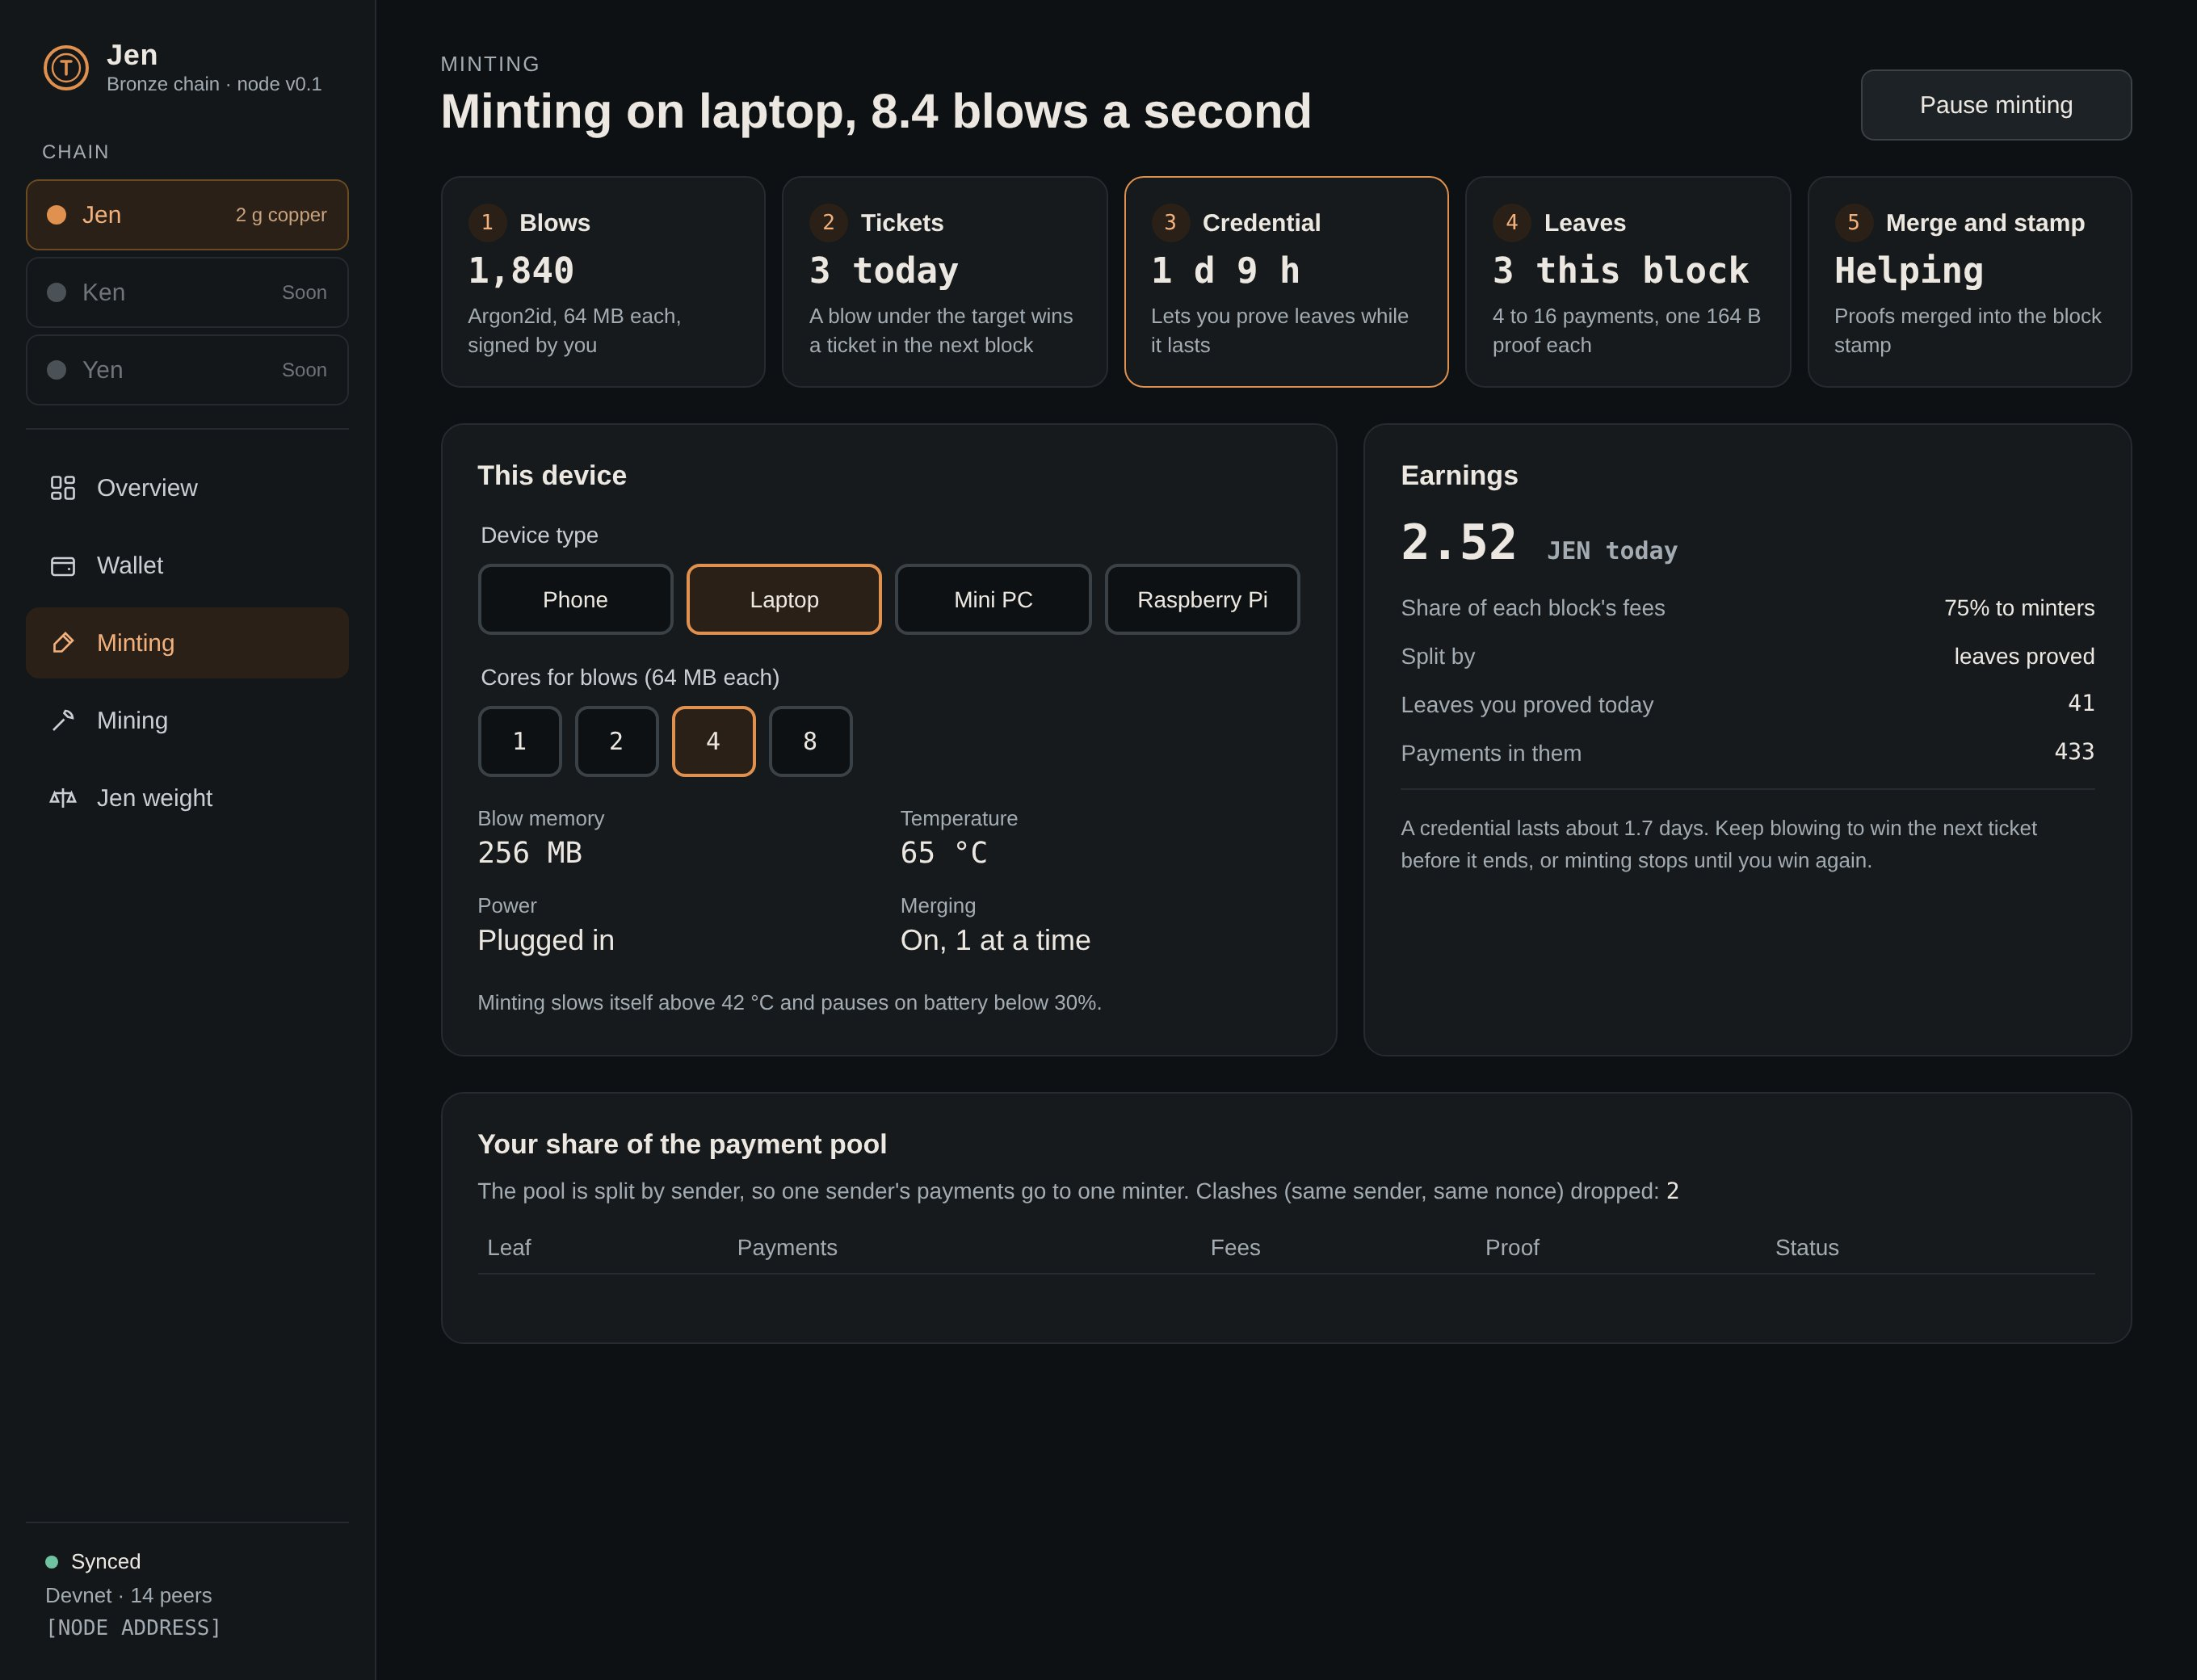
\includegraphics[width=\textwidth]{figs/ui_mint.jpg}
\caption{Minting: blows, tickets, credential, leaves and merging; device type and cores; the payment pool split by sender.}
\end{subfigure}\hfill
\begin{subfigure}{0.26\textwidth}\centering
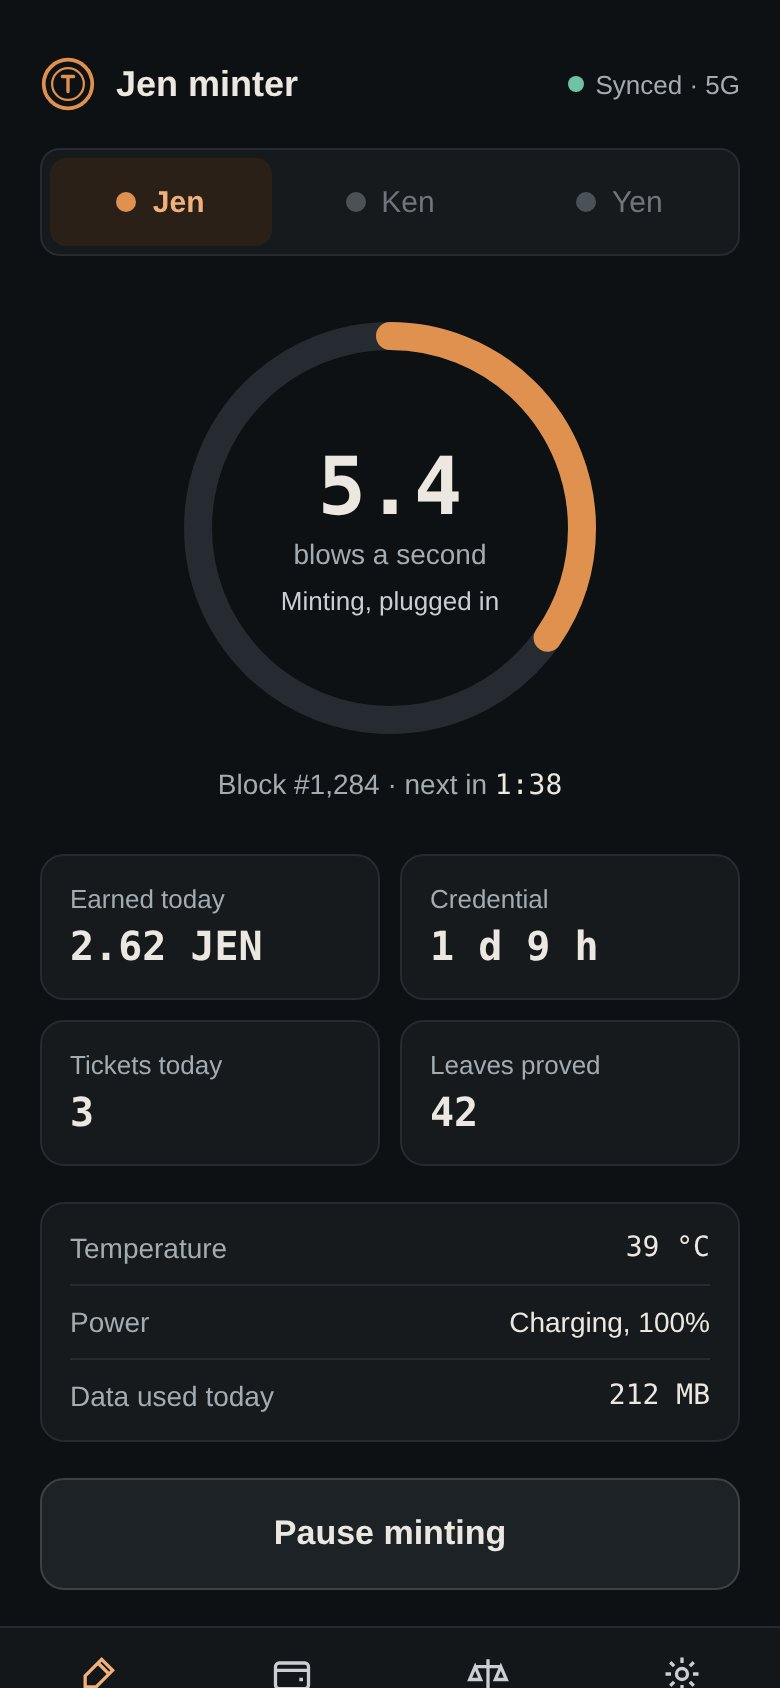
\includegraphics[width=\textwidth]{figs/ui_phone.jpg}
\caption{Phone minter (Android).}
\end{subfigure}
\caption{The Jen v1 interface prototype (sample data). Continued in Figure~\ref{fig:ui2}.}
\label{fig:ui}
\end{figure}

\begin{figure}[tbp]
\centering
\begin{subfigure}{\textwidth}\centering
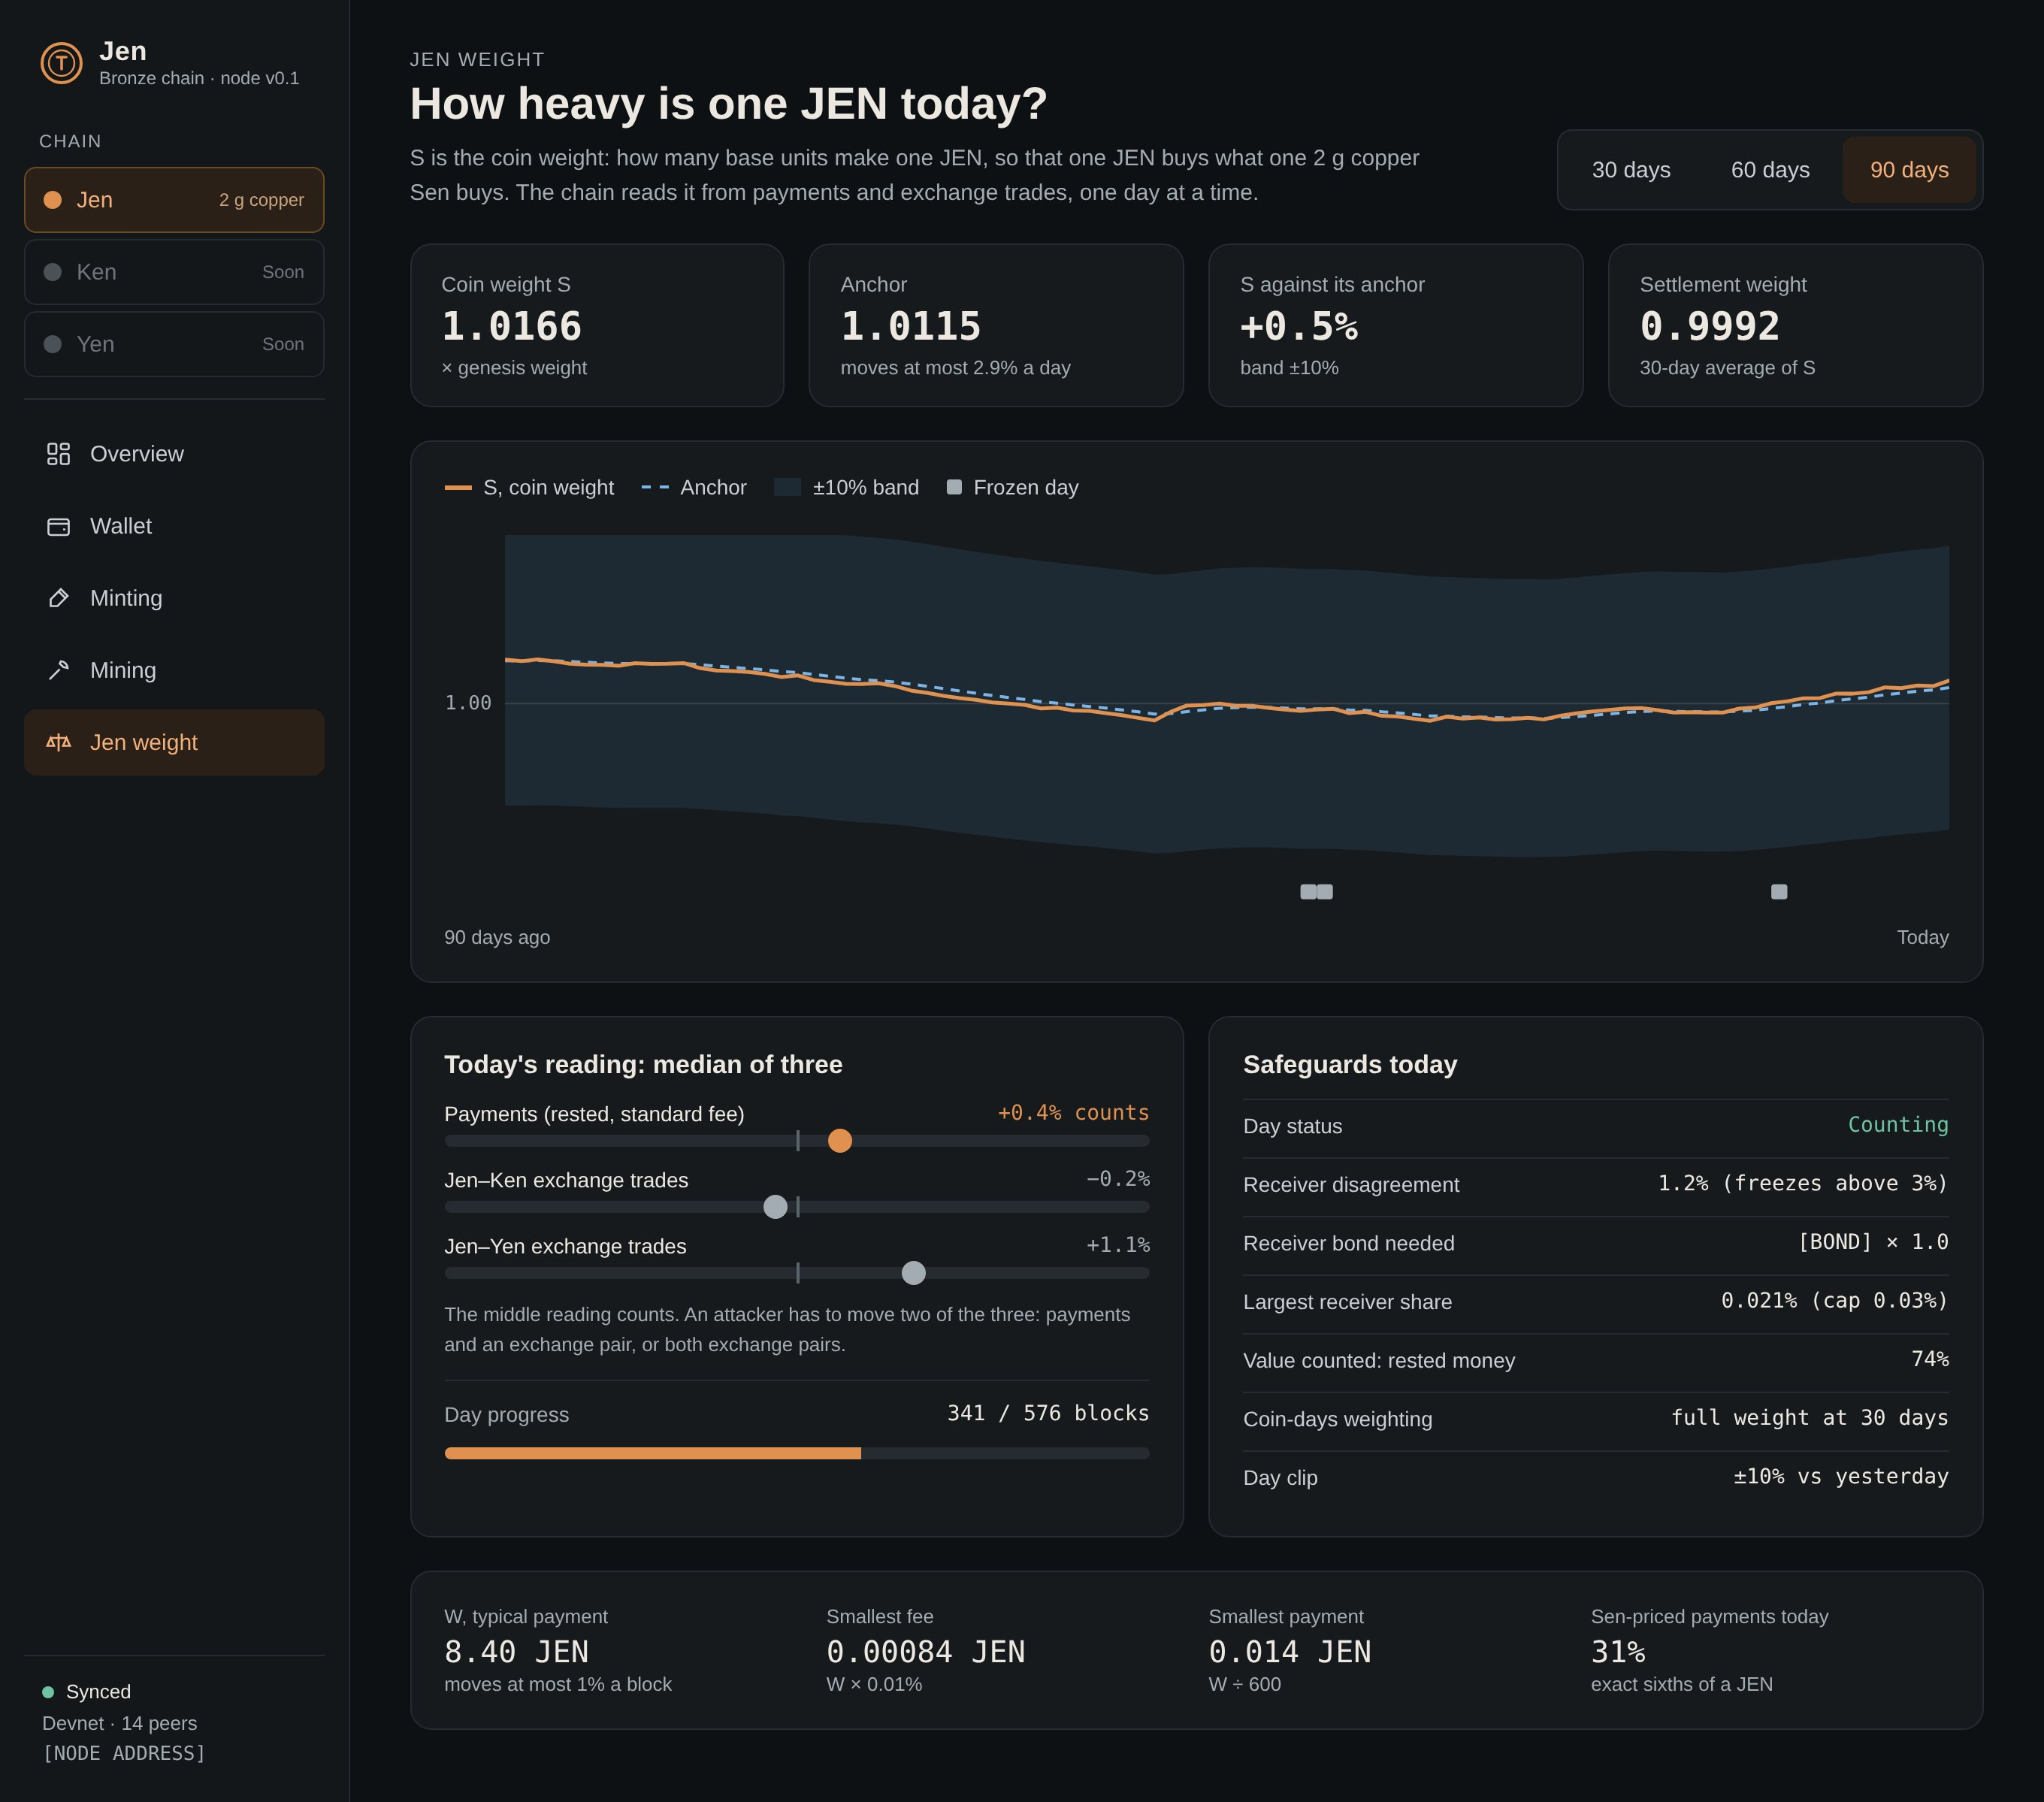
\includegraphics[width=0.98\textwidth]{figs/ui_weight.jpg}
\caption{Jen weight: $S$ against its anchor and band, today's three readings, the safeguards and the fee measure ($W$, since removed, Section~\ref{sec:w}).}
\end{subfigure}\\[8pt]
\begin{subfigure}{0.49\textwidth}\centering
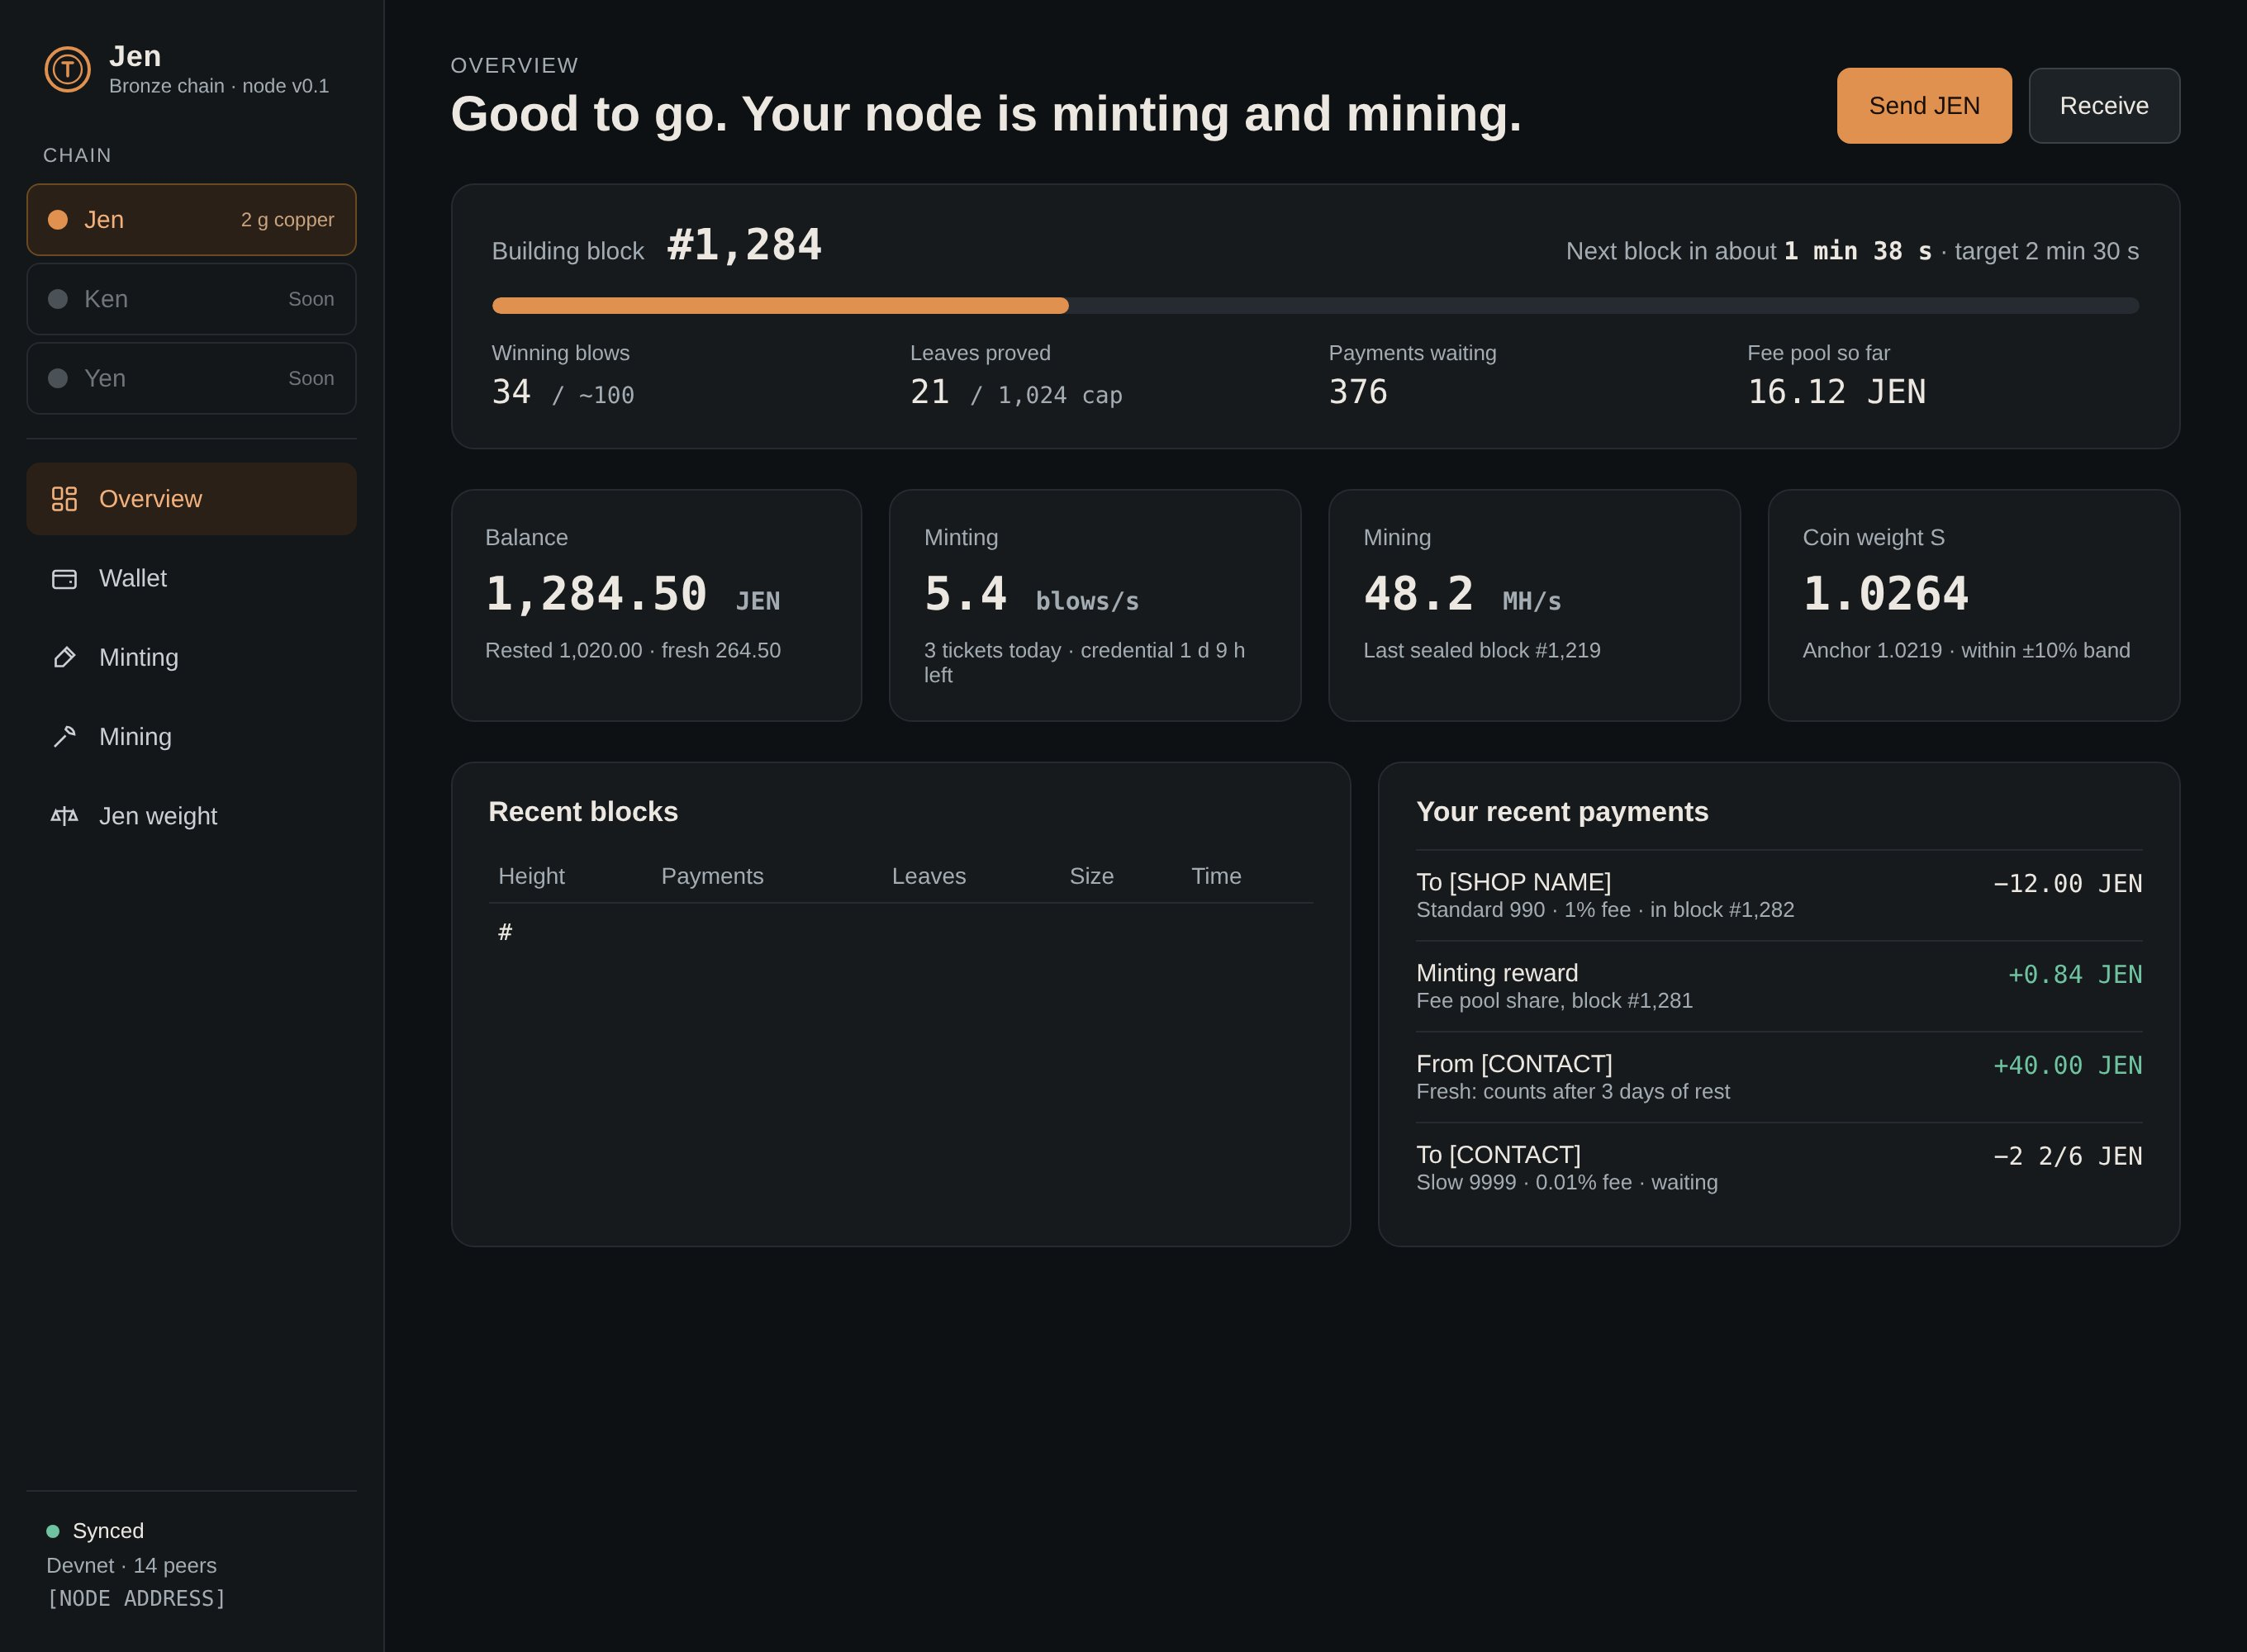
\includegraphics[width=\textwidth]{figs/ui_main.jpg}
\caption{Overview.}
\end{subfigure}\hfill
\begin{subfigure}{0.49\textwidth}\centering
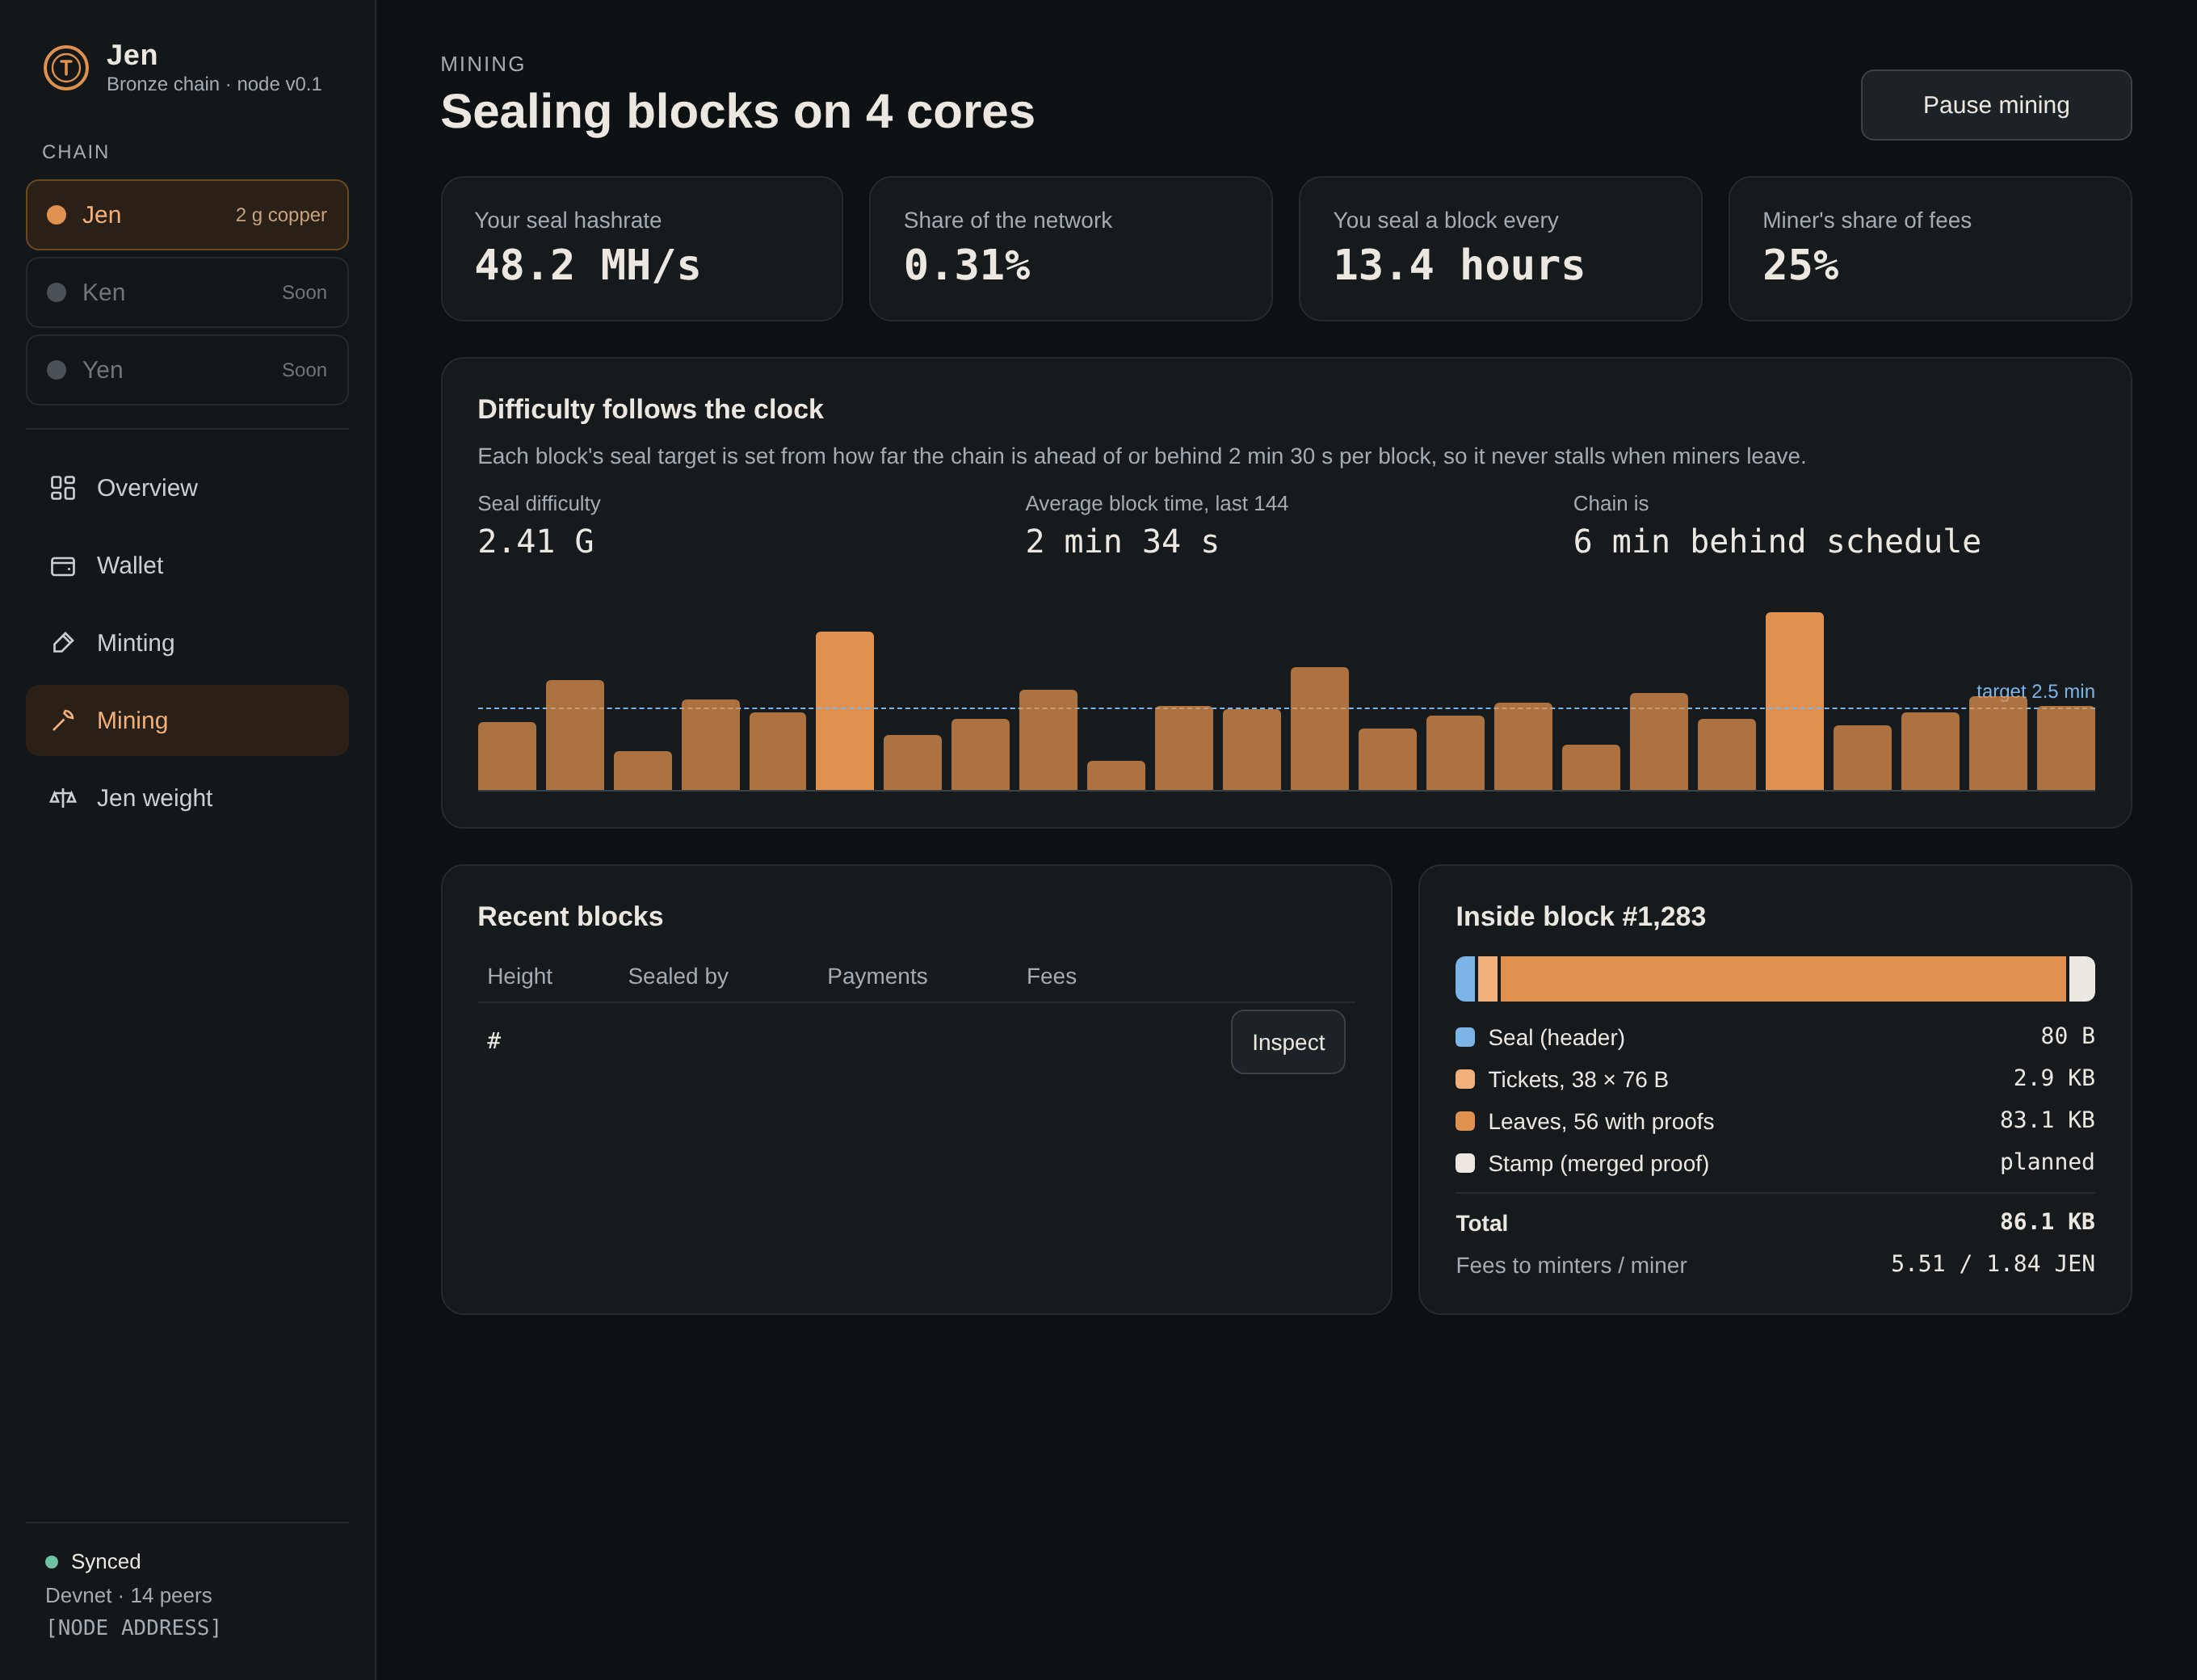
\includegraphics[width=\textwidth]{figs/ui_mine.jpg}
\caption{Mining: seal hashrate, time-based difficulty, block contents.}
\end{subfigure}
\caption{The Jen v1 interface prototype, continued.}
\label{fig:ui2}
\end{figure}

%=====================================================================
\FloatBarrier
\section{Economics and related work}\label{sec:econ}

\paragraph{Three roles separated.} Zen separates three roles that metal money historically combined. Physical coins of fixed weight are a store of value held privately. Electronic coins are the medium of payment. Each chain's $S$ states the electronic coin's value in grams of its metal.

\paragraph{Small change.} For centuries full-weight small coins were chronically scarce because they cost relatively more to mint \cite{sargentvelde}. The electronic Jen supplies small change in sixths of a Sen, at no minting cost, and in fractions of that over channels.

\paragraph{Fisher's compensated dollar.} Irving Fisher proposed fixing nothing but the dollar's purchasing power and varying its gold weight each month, with a 1\% spread so speculation could not profit \cite{fisher1914,fisher1920}; a modern comparison finds it would have cut price uncertainty by an order of magnitude \cite{bordo}. Zen follows the same logic in reverse: the stamped coins stay fixed, the electronic unit's weight floats with what the metal buys, and the anchor and band play the role of Fisher's spread.

\paragraph{Lessons from failed self-regulating money.} Designs that defended a peg by minting a second token failed through self-reinforcing runs: Terra (about \$50bn, May 2022) \cite{terra}, Iron Finance \cite{ironfinance}, Basis Cash \cite{basiscash} and NuBits \cite{nubits}. Zen has no second token defending a price and no collateral to liquidate, so its failure mode is mismeasurement or drift, not a death spiral. Three lessons still apply: lagging prices must not trigger automatic conversions (hence settlement at the 30-day average); coin age is useful but can be saved up and spent at once (held here by the cap, the middle-20\% reading and the band); and thin markets are cheap to move \cite{mango,uniswap}, hence a minimum exchange volume and a discount for payments created by the block's own producers (open).

\begin{table}[htbp]
\centering\footnotesize
\begin{tabularx}{\textwidth}{>{\raggedright\arraybackslash}p{3.0cm} Y Y Y}
\toprule
\textbf{Family} & \textbf{Examples} & \textbf{Where trust sits} & \textbf{Difference from Zen}\\
\midrule
Metal held by a custodian & e-gold, PAX Gold, Tether Gold & custodian, auditor & Zen's coin is not a claim on anyone's metal\\
Collateral + price feed & BitShares, Synthetix sXAU & feed publishers & no collateral, no feed\\
Rebasing to a target & Ampleforth & external oracle & input is the chain's own payments\\
Price from own payments & UTXOracle, brk\_oracle & nobody; outside consensus & read inside consensus, with a protocol grid (sixths) and defences\\
Staked reporters & SchellingCoin, UMA, Chainlink & stake-weighted reporters & no reporters to bribe\\
Issuance from history & Komi \& Tatekawa & consensus & steers issuance, sets no peg\\
Commodity money in theory & Fisher, Hayek, Graham, Keynes & a mint or buffer stock & no agent; the weight floats by consensus\\
\bottomrule
\end{tabularx}
\caption{Related work \cite{egold,paxg,bitusd,synthetix,ampleforth,utxoracle,brk,schellingcoin,komi,hayek,ussher}. The novelty claim rests on a limited literature search with no patent search and means ``no prior design found''.}
\label{tab:related}
\end{table}

%=====================================================================
\section{Security summary}\label{sec:security}

\begin{center}\begin{minipage}{\textwidth}\centering
\centering\small
\begin{tabularx}{\textwidth}{l Y Y}
\toprule
\textbf{Attack} & \textbf{Defence} & \textbf{Evidence}\\
\midrule
Stealing or outsourcing blows & each blow is signed by the minter's key & forged proofs and stolen blows rejected (simulation, 1,000 minters; devnet)\\
Forged leaf proof & proofs verified by every node; public inputs bind state roots, fees, prover & rejected on devnets with real proofs\\
Double spend via two minters & rank order; the state leaf skips a used (sender, nonce) & devnet supply exact; skipped in the Rust block (measured)\\
Builder changing a signed payment & state leaf re-hashes the signed fields against the signature leaf & no proof produced (measured)\\
Builder paying itself or others too much & nodes recompute the payout list; credits must match exactly & block rejected (measured)\\
Reusing a seal or swapping the miner address & commitment covers the coinbase and the body & rejected (measured)\\
A lock operation the node refuses & each operation family has its own circuit; the merge accepts only their four keys & 583 rule-breaking tries, none proves a refused operation (testnet)\\
A claim without a real foreign payment & every node checks the payment proof; the stamp binds its digest to the claim and the signature & rejected if the proof is wrong; not checked inside the stamp (testnet)\\
Overflowing a balance check & balance, amount and fee compared in 128-bit integers; money values below $2^{62}$ in circuits & wrapped sum refused (testnet, internal review)\\
Replaying a vault claim on another chain & the chain id is in the signed message & refused on the other chain (testnet)\\
Copying a sealed network request & one-time key kept in a replay cache for two time windows & copy inside the window refused (testnet)\\
A heavier-looking chain with less work & cross-chain follower keeps the chain with most cumulative work & rule tested (testnet)\\
Forged signature & checked inside the leaf proof, $s<n$, no exceptional curve cases & no proof produced (measured)\\
Replaying a signed payment & nonce in the signed message, incremented by the proof & no proof produced (measured)\\
Withholding or changing block data & stamp commits to a hash of the payments; nodes replay them & one changed byte rejected (measured)\\
Reusing a stamp for another block & public values bind roots, fees, count and data & rejected by the Groth16 verifier (measured)\\
One prover filling blocks & leaf quota and split pool & 15$\times$ faster prover: 99\% $\to$ 23\% of leaves (devnet)\\
Hidden chain with sealing power & two-factor fork choice & 3$\times$ sealing, 50\% minting: 59\% of honest weight (devnet)\\
Lowering one's own blow difficulty & gate and fork choice by minting work & attacker reached 58\% of honest work (devnet)\\
Faking congestion to resize & fee pool paid forward; grow only when full & --\\
Pushing $S$ & layered defences (Table~\ref{tab:layers}) & $\le$13\%/week; \$0.5M/month at 12\% (simulated)\\
Locking out small payers & fee limits in coins (0.01 coin; $\tfrac16$~\JEN{} smallest payment), not in typical payment sizes & --\\
Launch stall & time-based difficulty & block 100 in 10 h instead of 28 h (simulated)\\
\bottomrule
\end{tabularx}
\captionof{table}{Attacks and defences across the system.}
\end{minipage}\end{center}

%=====================================================================
\FloatBarrier
\section{Open problems and roadmap}\label{sec:open}

\begin{enumerate}
\item \textbf{The stamp in production.} Benchmarked (Section~\ref{sec:stamp}): one 196-byte proof per block, with signatures inside. Done: one key for every block size (a universal merge circuit), new and closed accounts, the chain id and prover credits inside the circuit, split signature and state leaves, one key per person for payments and blows, payouts inside the proof, the peg's account fields in the leaf, a Bitcoin-exact seal for Stratum pools, the rule that every block carries its stamp, and, on the Rust test network, every lock operation (vault, channel, order with auctions and claim, factory) inside the same stamp, with a soundness battery of 583 tries. Still open: a \textbf{public multi-party Groth16 ceremony} for the final circuit (the test key was made by one machine and is not safe for value), the foreign payment proof of an order claim inside the circuit, a builder benchmark on a many-core GPU server, phone proving tests, fuzzing of every decoder, and an external audit of circuits and consensus. The 70\,KB Plonky2 stamp, which needs no ceremony, is the fallback.
\item \textbf{The young chain.} Jen runs alone for about 3.5 years with little traffic and no exchange: a slower anchor, a longer rest and a lower cap while volume is low, a launch simulation, and the time-based difficulty for blows and seals.
\item \textbf{Faster honest following.} When payments and both exchange readings agree on a move, let the anchor move faster (for example 3 times); an attacker cannot fake all three at once.
\item \textbf{Ordinary-side attacks.} Fake ordinary payments (the gram side of the reading) are not yet simulated.
\item \textbf{Block producers.} Discount payments created by the block's own miner or minter, and count rest periods in blocks.
\item \textbf{Channels and the sample.} Payments kept in channels never reach the reading, so the sample shrinks and skews toward large flows as channels succeed. Which channel events count as observations is open.
\item \textbf{Thin exchange pairs.} A minimum daily volume before an exchange reading counts.
\item \textbf{Adaptive attackers.} Aged balances spent at once, switching direction when defenders arrive, staying just under each trigger.
\item \textbf{Pricing practice.} Wallets that quote coin prices and ratios from metal prices by default, since the peg converges only when most coin-priced value is set from the metal.
\item \textbf{A formal bound.} A cost-of-corruption bound for the peg, as Bitcoin states the attacker's catch-up probability.
\item \textbf{Open parameters.} Whether $V$ applies to Yen's first blocks; the reward curve (smooth or step table); the fee split as rewards fade; leaf size at launch; the seal hash; and the exchange version at launch (Table~\ref{tab:opendec}).
\end{enumerate}

\begin{table}[htbp]
\centering\small
\begin{tabularx}{\textwidth}{Y Y Y}
\toprule
\textbf{Question} & \textbf{Options} & \textbf{Recommendation}\\
\midrule
Random factor in Yen's first blocks & random from block 1, or $V=1$ for $\approx$100 blocks & fixed at first\\
Reward curve & smooth (Yen limit $\approx$7,255) or step table (10,080) & smooth curve\\
Fee split minters / miner & fixed 75/25, or miner share rising as the reward fades & rising miner share\\
Leaf size at launch & 4, 8 or 16 payments & 4 for phones, 16 for desktops\\
Proof system & Plonky2 leaves and merges wrapped in one Groth16 stamp (ceremony), or the 70\,KB Plonky2 stamp (no setup) & Plonky2 + Groth16 stamp, with a public ceremony\\
Hash inside proofs & MiMC, Poseidon or Poseidon2 & Poseidon over Goldilocks; over BN254 in the last layer\\
Seal hash & SHA-256 or a hash that resists dedicated chips & to research\\
Exchange at launch & reserve--pay--claim, or batch auctions & reserve--pay--claim first\\
\bottomrule
\end{tabularx}
\caption{Open decisions (specification 11).}
\label{tab:opendec}
\end{table}

%=====================================================================
\section{Conclusion}
Zen proposes metal money with no vault and no price feed. Three physical coins set the reference; three chains read their value from the way people pay, and defend that reading with rules whose cost to an attacker can be measured. Phones mint the blocks and share the fees, ordinary SHA-256 hardware seals them, and channels, the exchange and Zen Net carry the payments that do not need to be on a chain. The simulations in this paper suggest that the peg can be made expensive to move and quick to restore, provided most coin-priced shops price from the metal itself. A Rust implementation now runs the three chains on a test network, with the merge proof carrying payments and every lock operation. The next steps are a public Groth16 ceremony, fuzzing and an outside audit, a launch simulation, and a public testnet open to phones.

\paragraph{Author's note.} Zen, its six coins (Gold Ren, Silver Ten and Copper Sen; Golden Yen, Silver Ken and Bronze Jen) and the designs in this paper are the work of Justus L. Ludovic. Prototype code: the Rust node \texttt{zenproof} (rounds 1 to 55), \texttt{zen\_minting.py}, \texttt{pom\_simulation.py}, \texttt{pom-leaf} (Go, gnark), the Jen-0 to Jen-0.11 devnets and the peg simulations listed in Appendix~\ref{app:sims}.

%=====================================================================
\begin{thebibliography}{99}\small
\setlength{\itemsep}{1pt}
\bibitem{nakamoto} S.~Nakamoto, \emph{Bitcoin: A Peer-to-Peer Electronic Cash System}, 2008. \url{https://bitcoin.org/bitcoin.pdf}
\bibitem{yermack} D.~Yermack, \emph{Is Bitcoin a Real Currency? An Economic Appraisal}, NBER w19747, 2013. \url{https://www.nber.org/papers/w19747}
\bibitem{klagesmundt} A.~Klages-Mundt, D.~Harz, L.~Gudgeon, J.-Y.~Liu, A.~Minca, \emph{Stablecoins 2.0}, AFT 2020. \url{https://arxiv.org/pdf/2006.12388v2}
\bibitem{caldarelli} G.~Caldarelli, \emph{Understanding the Blockchain Oracle Problem}, Information 11(11), 2020. \url{https://www.mdpi.com/2078-2489/11/11/509/htm}
\bibitem{douceur} J.~R.~Douceur, \emph{The Sybil Attack}, IPTPS 2002. \url{https://www.microsoft.com/en-us/research/publication/the-sybil-attack/}
\bibitem{egold-doj} US Department of Justice, e-gold plea, July 2008. \url{https://www.justice.gov/archive/opa/pr/2008/July/08-crm-635.html}
\bibitem{egold} e-gold (overview). \url{https://en.wikipedia.org/wiki/E-gold}
\bibitem{paxg} Gold-backed stablecoins overview (PAXG, XAUt, KAU). \url{https://stablecoininsider.org/gold-backed-stablecoins/}
\bibitem{bitusd} The Block, \emph{bitUSD loses its peg}, 2019. \url{https://www.theblock.co/news/markets/2019-02-15-bitusd-hasnt-had-its-1-peg-for-more-than-two-months-11876}
\bibitem{synthetix} Synthetix, Chainlink price feeds for sXAU/sXAG. \url{https://blog.synthetix.io/chainlink-decentralizes-first-wave-of-synthetix-price-feeds/}
\bibitem{ampleforth} Chainlink, Ampleforth case study. \url{https://chain.link/case-studies/ampleforth}
\bibitem{utxoracle} UTXOracle: a decentralized approach to the oracle problem. \url{https://www.nasdaq.com/articles/utxoracle:-a-decentralized-approach-to-the-oracle-problem}
\bibitem{brk} brk\_oracle documentation. \url{https://docs.rs/crate/brk_oracle/0.3.4}
\bibitem{schellingcoin} V.~Buterin, \emph{SchellingCoin}, 2014. \url{https://blog.ethereum.org/2014/03/28/schellingcoin-a-minimal-trust-universal-data-feed}
\bibitem{komi} Komi \& Tatekawa, \emph{Consensus Algorithm Using Transaction History}, ePrint 2023/373. \url{https://eprint.iacr.org/2023/373.pdf}
\bibitem{nubits} Moneyness, \emph{The end of a stablecoin} (NuBits), 2016. \url{https://www.moneyness.ca/2016/08/end-of-stablecoin.html}
\bibitem{mango} Davis Wright Tremaine, CFTC action on Mango Markets, 2023. \url{https://dwt.com/blogs/financial-services-law-advisor/2023/01/cftc-decentralized-manipulation-crypto}
\bibitem{terra} J.~Liu, I.~Makarov, A.~Schoar, \emph{Anatomy of a Run: The Terra Luna Crash}, NBER w31160. \url{https://www.nber.org/papers/w31160}
\bibitem{ironfinance} Finematics, \emph{Bank run in DeFi: Iron Finance explained}. \url{https://finematics.com/bank-run-in-defi-iron-finance-explained/}
\bibitem{basiscash} Zhao, Li \& Yuan, Basis Cash model checking, arXiv 2101.08423. \url{https://ar5iv.arxiv.org/html/2101.08423}
\bibitem{peercoin} S.~King, S.~Nadal, \emph{PPCoin: Peer-to-Peer Crypto-Currency with Proof-of-Stake}, 2012. \url{https://raw.githubusercontent.com/papers-we-love/papers-we-love/refs/heads/main/digital_currency/peercoin.pdf}
\bibitem{uniswap} Uniswap Labs, \emph{Uniswap v3 TWAP oracles in proof of stake}. \url{https://blog.uniswap.org/uniswap-v3-oracles}
\bibitem{velde} F.~Velde, \emph{The Crime of 1873: Back to the Scene}, Chicago Fed WP 2002-29. \url{https://www.chicagofed.org/~/media/publications/working-papers/2002/wp2002-29-pdf.pdf}
\bibitem{sargentvelde} T.~Sargent, F.~Velde, \emph{The Evolution of Small Change}, Chicago Fed WP 97-13. \url{https://www.chicagofed.org/~/media/publications/working-papers/1997/wp97-13-pdf.pdf}
\bibitem{bordo} M.~Bordo, R.~Dittmar, W.~Gavin, \emph{Gold, Fiat Money, and Price Stability}, NBER w10171. \url{https://www.nber.org/papers/w10171}
\bibitem{eichengreen} B.~Eichengreen, \emph{Golden Fetters}, Oxford University Press, 1992. \url{https://www.nber.org/books-and-chapters/golden-fetters-gold-standard-and-great-depression-1919-1939}
\bibitem{fisher1914} I.~Fisher, \emph{Objections to a Compensated Dollar Answered}, QJE, 1914. \url{https://people.wku.edu/charles.smith/wallace/zFisherI1914.pdf}
\bibitem{fisher1920} I.~Fisher, \emph{Stabilizing the Dollar}, 1920. \url{https://fraser.stlouisfed.org/files/docs/publications/books/stabilizing_fisher.pdf}
\bibitem{hayek} F.~A.~Hayek, commodity reserve currency (AIER). \url{https://aier.org/article/hayeks-commodity-reserve-currency/}
\bibitem{ussher} L.~Ussher, \emph{Keynes, Graham and Kaldor on commodity reserve currency}, INET. \url{https://ineteconomics.org/research/research-papers/combining-international-monetary-reform-with-commodity-buffer-stocks-keynes-graham-and-kaldor}
\bibitem{bis2018} BIS Annual Economic Report 2018, ch. V. \url{https://bis.org/publ/arpdf/ar2018e5.htm}
\bibitem{burchert} C.~Burchert, C.~Decker, R.~Wattenhofer, \emph{Scalable funding of Bitcoin micropayment channel networks}, Royal Society Open Science, 2018. \url{https://doaj.org/article/39e059f7493041ed8b6bb6e47c5887a4}
\bibitem{superscalar} SuperScalar: an implementation report, Delving Bitcoin, July 2026. \url{https://delvingbitcoin.org/t/superscalar-an-implementation-report/2705}
\bibitem{eltoo} C.~Decker, R.~Russell, O.~Osuntokun, \emph{eltoo: A Simple Layer2 Protocol for Bitcoin}. \url{https://blockstream.com/eltoo.pdf}
\bibitem{lightning} J.~Poon, T.~Dryja, \emph{The Bitcoin Lightning Network}. \url{https://lightning.network/lightning-network-paper.pdf}
\bibitem{sok} L.~Gudgeon et al., \emph{SoK: Layer-Two Blockchain Protocols}, ePrint 2019/360. \url{https://eprint.iacr.org/2019/360}
\end{thebibliography}

%=====================================================================
\appendix
\section{Simulation methods}\label{app:sims}

All simulations are small, deterministic (seeded) models written for this design; they are evidence about the rules, not predictions about markets. Code is in the accompanying archive.

\paragraph{Detection model (\texttt{detect9.py}).} Three chains, nine hourly readings: each chain's payment reading (noise 4.9\% an hour, 1\% a day) and its readings through its two exchange pairs (3.3\% an hour, 0.67\% a day); three times the noise for thin markets. Biases: fake payments shift one payment reading; wrong-ratio orders on a pair shift that pair's two readings in opposite directions. Detection fits the means of the last 1, 3, 6, 12 and 24 hours with every set of 0, 1 or 2 biased components (unknown true values per chain), with a penalty per component set so that quiet runs raise about one false alarm in five years. Attribution refits the 48 hours ending a day after the alarm, with a penalty of 10 per component. 400 runs of 14 days per point.

\paragraph{Market model of the peg (\texttt{daywin.js}, \texttt{volsim.js}, \texttt{volsim2.js}, \texttt{defend.js}, \texttt{auto.js}, \texttt{tri2.js}, \texttt{converge.js}).} Days of payments on Jen at one million payments a day, 30\% of them coin-priced; goods lognormal around 2~Sen; honest money's age exponential with a mean of 20 days (assumed); 85\%, 75\% or 60\% of honest money rested for rests of 1, 3 or 7 days (assumed). The true value of a Sen in base units follows a random walk. Attackers choose the offset and direction that push hardest and, where receivers matter, spread over as many bonded accounts as the cap requires; their costs are fees, 5\% a year interest on locked money and burned penalties. The three-chain model adds coin-priced batch auctions per pair with metal prices quoted at a 2\% spread. Largest moves are reported as the largest ratio between $S$ and the true value during or after the attack.

\paragraph{Launch model (\texttt{launch\_sim.py}).} Jen blocks every 150\,s on average; block discovery is a Poisson process with rate hashrate/difficulty. Per-block rule: after each block, difficulty $\times\,\mathrm{clamp}(T/\Delta t, 1/1.125, 1.125)$. Time-based rule: $D(t) = D_{\mathrm{ref}}\,2^{(NT-t)/h}$ with $h=1$ hour, evaluated in 5-second steps. Five seeds per rule.

\paragraph{Proof benchmark (\texttt{zkbench}).} Rust, Plonky2 1.1 for leaves, merges, the shrink and the BN254 layer, and gnark v0.16.4 (Go) for the Groth16 stamp, on a 2-core cloud server with 7\,GB of RAM and 12\,GB of swap for the setup; timings vary by about 30\% between runs on that machine. Each leaf updates a depth-32 Poseidon account tree for sender and receiver, checks the fee limits with range checks, and checks a Schnorr signature on EcGFp5. The tests are a forged $s$, a replayed payment, a changed public value, a changed proof value, a changed byte of block data, and one block's proof against another block's public values. Code and results are in the accompanying archive.

\paragraph{Operation circuits and their tests (\texttt{zenproof}).} The four operation leaves, the four-key merge, a shrink and BN254 layer rebuilt over it, and a new Groth16 setup (4,203,150 constraints, 17 public values, 1,008-byte verifying key) were built and run on the same machine with a 10\,GB swap file; the BN254 layer proves in 54.6\,s. A node holding only the verifying key accepted real stamps of blocks that carried an order, a channel and a factory being made, then a reservation and the start of a member's exit, and refused a stamp with one byte changed. The soundness battery (\texttt{soundness.rs}) runs 583 mutated operations through the real prover; the whole suite of 137 tests passes (testnet).

\paragraph{Devnets.} Go prototypes Jen-0.5 to Jen-0.11 run as 4--24 nodes on shared test machines, with real Groth16 leaf proofs or proving simulated at a fixed time per leaf, as stated with each result.

\section{Glossary}
\begin{description}[leftmargin=3.1cm,labelwidth=2.9cm,labelindent=0pt,itemsep=1pt]
\item[Anchor] A slow copy of $S$ that moves at most 2.9\% a day; $S$ must stay within $\pm10\%$ of it.
\item[Blow] One signed Argon2id attempt (64\,MB) at the minting puzzle.
\item[Coin-priced] A payment of an exact number of sixths of a coin; the shop priced in coins.
\item[Coin-days] Weight of a counted payment by how long its money rested, up to 30 days.
\item[Builder] Turns minters' signature leaves into a block: state leaves, merges and the stamp; in practice a mining pool.
\item[Credential] The right to prove leaves, held while one's ticket is in the recent chain.
\item[Fineness / purity] A payment's fee rate written like metal purity (940 = 6\%, 9999 = 0.01\%); purity is the day's geometric mean.
\item[Leaf] A group of 4--16 payments with one zero-knowledge proof. An \emph{operation leaf} proves one vault, channel, order or factory operation.
\item[Lock] An account-tree leaf whose address is a digest of its terms: a vault, an order, a channel or a factory.
\item[Melt, stream, cast] Enter a channel, pay off-chain, settle back on-chain.
\item[$S$] The coin weight: base units per electronic coin, read so that one coin equals one physical coin.
\item[Seal] The miner's SHA-256 proof of work over Bitcoin's 80-byte header.
\item[Stamp] The single proof of a whole block: 196 bytes, checked in 2--4\,ms (benchmarked); it covers payments and, on the test network, lock operations.
\item[Ticket] A winning blow recorded in a block.
\item[$W$] The typical payment size; set the fee limits in earlier drafts, removed in October 2026.
\end{description}


\end{document}
